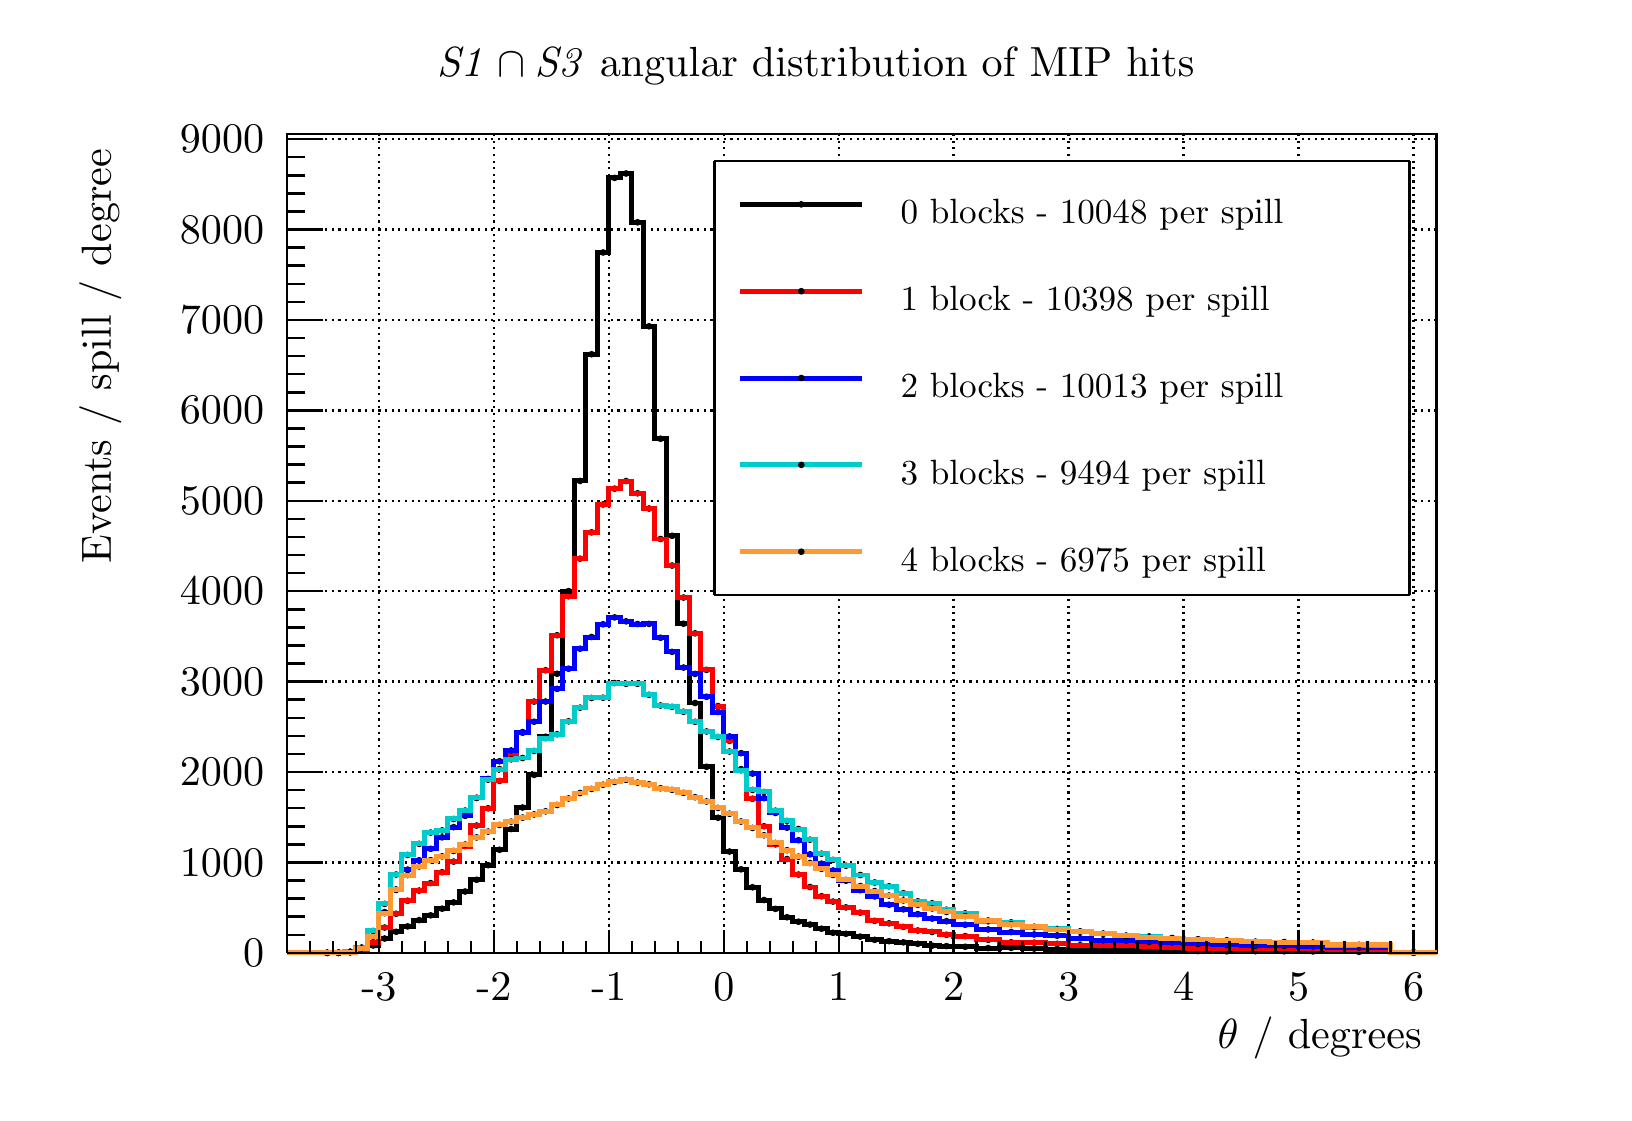
\begin{tikzpicture}
\pgfdeclareplotmark{cross} {
\pgfpathmoveto{\pgfpoint{-0.3\pgfplotmarksize}{\pgfplotmarksize}}
\pgfpathlineto{\pgfpoint{+0.3\pgfplotmarksize}{\pgfplotmarksize}}
\pgfpathlineto{\pgfpoint{+0.3\pgfplotmarksize}{0.3\pgfplotmarksize}}
\pgfpathlineto{\pgfpoint{+1\pgfplotmarksize}{0.3\pgfplotmarksize}}
\pgfpathlineto{\pgfpoint{+1\pgfplotmarksize}{-0.3\pgfplotmarksize}}
\pgfpathlineto{\pgfpoint{+0.3\pgfplotmarksize}{-0.3\pgfplotmarksize}}
\pgfpathlineto{\pgfpoint{+0.3\pgfplotmarksize}{-1.\pgfplotmarksize}}
\pgfpathlineto{\pgfpoint{-0.3\pgfplotmarksize}{-1.\pgfplotmarksize}}
\pgfpathlineto{\pgfpoint{-0.3\pgfplotmarksize}{-0.3\pgfplotmarksize}}
\pgfpathlineto{\pgfpoint{-1.\pgfplotmarksize}{-0.3\pgfplotmarksize}}
\pgfpathlineto{\pgfpoint{-1.\pgfplotmarksize}{0.3\pgfplotmarksize}}
\pgfpathlineto{\pgfpoint{-0.3\pgfplotmarksize}{0.3\pgfplotmarksize}}
\pgfpathclose
\pgfusepathqstroke
}
\pgfdeclareplotmark{cross*} {
\pgfpathmoveto{\pgfpoint{-0.3\pgfplotmarksize}{\pgfplotmarksize}}
\pgfpathlineto{\pgfpoint{+0.3\pgfplotmarksize}{\pgfplotmarksize}}
\pgfpathlineto{\pgfpoint{+0.3\pgfplotmarksize}{0.3\pgfplotmarksize}}
\pgfpathlineto{\pgfpoint{+1\pgfplotmarksize}{0.3\pgfplotmarksize}}
\pgfpathlineto{\pgfpoint{+1\pgfplotmarksize}{-0.3\pgfplotmarksize}}
\pgfpathlineto{\pgfpoint{+0.3\pgfplotmarksize}{-0.3\pgfplotmarksize}}
\pgfpathlineto{\pgfpoint{+0.3\pgfplotmarksize}{-1.\pgfplotmarksize}}
\pgfpathlineto{\pgfpoint{-0.3\pgfplotmarksize}{-1.\pgfplotmarksize}}
\pgfpathlineto{\pgfpoint{-0.3\pgfplotmarksize}{-0.3\pgfplotmarksize}}
\pgfpathlineto{\pgfpoint{-1.\pgfplotmarksize}{-0.3\pgfplotmarksize}}
\pgfpathlineto{\pgfpoint{-1.\pgfplotmarksize}{0.3\pgfplotmarksize}}
\pgfpathlineto{\pgfpoint{-0.3\pgfplotmarksize}{0.3\pgfplotmarksize}}
\pgfpathclose
\pgfusepathqfillstroke
}
\pgfdeclareplotmark{newstar} {
\pgfpathmoveto{\pgfqpoint{0pt}{\pgfplotmarksize}}
\pgfpathlineto{\pgfqpointpolar{44}{0.5\pgfplotmarksize}}
\pgfpathlineto{\pgfqpointpolar{18}{\pgfplotmarksize}}
\pgfpathlineto{\pgfqpointpolar{-20}{0.5\pgfplotmarksize}}
\pgfpathlineto{\pgfqpointpolar{-54}{\pgfplotmarksize}}
\pgfpathlineto{\pgfqpointpolar{-90}{0.5\pgfplotmarksize}}
\pgfpathlineto{\pgfqpointpolar{234}{\pgfplotmarksize}}
\pgfpathlineto{\pgfqpointpolar{198}{0.5\pgfplotmarksize}}
\pgfpathlineto{\pgfqpointpolar{162}{\pgfplotmarksize}}
\pgfpathlineto{\pgfqpointpolar{134}{0.5\pgfplotmarksize}}
\pgfpathclose
\pgfusepathqstroke
}
\pgfdeclareplotmark{newstar*} {
\pgfpathmoveto{\pgfqpoint{0pt}{\pgfplotmarksize}}
\pgfpathlineto{\pgfqpointpolar{44}{0.5\pgfplotmarksize}}
\pgfpathlineto{\pgfqpointpolar{18}{\pgfplotmarksize}}
\pgfpathlineto{\pgfqpointpolar{-20}{0.5\pgfplotmarksize}}
\pgfpathlineto{\pgfqpointpolar{-54}{\pgfplotmarksize}}
\pgfpathlineto{\pgfqpointpolar{-90}{0.5\pgfplotmarksize}}
\pgfpathlineto{\pgfqpointpolar{234}{\pgfplotmarksize}}
\pgfpathlineto{\pgfqpointpolar{198}{0.5\pgfplotmarksize}}
\pgfpathlineto{\pgfqpointpolar{162}{\pgfplotmarksize}}
\pgfpathlineto{\pgfqpointpolar{134}{0.5\pgfplotmarksize}}
\pgfpathclose
\pgfusepathqfillstroke
}
\definecolor{c}{rgb}{1,1,1};
\draw [color=c, fill=c] (0,0) rectangle (20,13.5143);
\draw [color=c, fill=c] (3.28571,1.77143) rectangle (17.8857,12.1714);
\definecolor{c}{rgb}{0,0,0};
\draw [c,line width=0.9] (3.28571,1.77143) -- (3.28571,12.1714) -- (17.8857,12.1714) -- (17.8857,1.77143) -- (3.28571,1.77143);
\definecolor{c}{rgb}{1,1,1};
\draw [color=c, fill=c] (3.28571,1.77143) rectangle (17.8857,12.1714);
\definecolor{c}{rgb}{0,0,0};
\draw [c,line width=0.9] (3.28571,1.77143) -- (3.28571,12.1714) -- (17.8857,12.1714) -- (17.8857,1.77143) -- (3.28571,1.77143);
\draw [c,line width=0.9] (3.28571,1.77143) -- (17.8857,1.77143);
\draw [c,dash pattern=on 0.80pt off 1.60pt ,line width=0.9] (4.45371,12.1714) -- (4.45371,1.77143);
\draw [c,dash pattern=on 0.80pt off 1.60pt ,line width=0.9] (5.91371,12.1714) -- (5.91371,1.77143);
\draw [c,dash pattern=on 0.80pt off 1.60pt ,line width=0.9] (7.37371,12.1714) -- (7.37371,1.77143);
\draw [c,dash pattern=on 0.80pt off 1.60pt ,line width=0.9] (8.83371,12.1714) -- (8.83371,1.77143);
\draw [c,dash pattern=on 0.80pt off 1.60pt ,line width=0.9] (10.2937,12.1714) -- (10.2937,1.77143);
\draw [c,dash pattern=on 0.80pt off 1.60pt ,line width=0.9] (11.7537,12.1714) -- (11.7537,1.77143);
\draw [c,dash pattern=on 0.80pt off 1.60pt ,line width=0.9] (13.2137,12.1714) -- (13.2137,1.77143);
\draw [c,dash pattern=on 0.80pt off 1.60pt ,line width=0.9] (14.6737,12.1714) -- (14.6737,1.77143);
\draw [c,dash pattern=on 0.80pt off 1.60pt ,line width=0.9] (16.1337,12.1714) -- (16.1337,1.77143);
\draw [c,dash pattern=on 0.80pt off 1.60pt ,line width=0.9] (17.5937,12.1714) -- (17.5937,1.77143);
\draw [c,dash pattern=on 0.80pt off 1.60pt ,line width=0.9] (4.45371,12.1714) -- (4.45371,1.77143);
\draw [c,dash pattern=on 0.80pt off 1.60pt ,line width=0.9] (17.5937,12.1714) -- (17.5937,1.77143);
\draw [c,line width=0.9] (3.28571,1.77143) -- (3.28571,12.1714);
\draw [c,dash pattern=on 0.80pt off 1.60pt ,line width=0.9] (17.8857,1.77143) -- (3.28571,1.77143);
\draw [c,dash pattern=on 0.80pt off 1.60pt ,line width=0.9] (17.8857,2.91963) -- (3.28571,2.91963);
\draw [c,dash pattern=on 0.80pt off 1.60pt ,line width=0.9] (17.8857,4.06783) -- (3.28571,4.06783);
\draw [c,dash pattern=on 0.80pt off 1.60pt ,line width=0.9] (17.8857,5.21603) -- (3.28571,5.21603);
\draw [c,dash pattern=on 0.80pt off 1.60pt ,line width=0.9] (17.8857,6.36423) -- (3.28571,6.36423);
\draw [c,dash pattern=on 0.80pt off 1.60pt ,line width=0.9] (17.8857,7.51243) -- (3.28571,7.51243);
\draw [c,dash pattern=on 0.80pt off 1.60pt ,line width=0.9] (17.8857,8.66063) -- (3.28571,8.66063);
\draw [c,dash pattern=on 0.80pt off 1.60pt ,line width=0.9] (17.8857,9.80883) -- (3.28571,9.80883);
\draw [c,dash pattern=on 0.80pt off 1.60pt ,line width=0.9] (17.8857,10.957) -- (3.28571,10.957);
\draw [c,dash pattern=on 0.80pt off 1.60pt ,line width=0.9] (17.8857,12.1052) -- (3.28571,12.1052);
\draw [c,dash pattern=on 0.80pt off 1.60pt ,line width=0.9] (17.8857,12.1052) -- (3.28571,12.1052);
\definecolor{c}{rgb}{0,0,0.6};
\draw [c,line width=0.9] (3.28571,1.77143) -- (3.43171,1.77143) -- (3.43171,1.77143) -- (3.57771,1.77143) -- (3.57771,1.77143) -- (3.72371,1.77143) -- (3.72371,1.77143) -- (3.86971,1.77143) -- (3.86971,1.77143) -- (4.01571,1.77143) --
 (4.01571,1.77143) -- (4.16171,1.77143) -- (4.16171,1.77143) -- (4.30771,1.77143) -- (4.30771,1.77143) -- (4.45371,1.77143) -- (4.45371,1.77143) -- (4.59971,1.77143) -- (4.59971,1.77143) -- (4.74571,1.77143) -- (4.74571,1.77143) -- (4.89171,1.77143)
 -- (4.89171,1.77143) -- (5.03771,1.77143) -- (5.03771,1.77143) -- (5.18371,1.77143) -- (5.18371,1.77143) -- (5.32971,1.77143) -- (5.32971,1.77143) -- (5.47571,1.77143) -- (5.47571,1.77143) -- (5.62171,1.77143) -- (5.62171,1.77143) --
 (5.76771,1.77143) -- (5.76771,1.77143) -- (5.91371,1.77143) -- (5.91371,1.77143) -- (6.05971,1.77143) -- (6.05971,1.77143) -- (6.20571,1.77143) -- (6.20571,1.77143) -- (6.35171,1.77143) -- (6.35171,1.77143) -- (6.49771,1.77143) -- (6.49771,1.77143)
 -- (6.64371,1.77143) -- (6.64371,1.77143) -- (6.78971,1.77143) -- (6.78971,1.77143) -- (6.93571,1.77143) -- (6.93571,1.77143) -- (7.08171,1.77143) -- (7.08171,1.77143) -- (7.22771,1.77143) -- (7.22771,1.77143) -- (7.37371,1.77143) --
 (7.37371,1.77143) -- (7.51971,1.77143) -- (7.51971,1.77143) -- (7.66571,1.77143) -- (7.66571,1.77143) -- (7.81171,1.77143) -- (7.81171,1.77143) -- (7.95771,1.77143) -- (7.95771,1.77143) -- (8.10371,1.77143) -- (8.10371,1.77143) -- (8.24971,1.77143)
 -- (8.24971,1.77143) -- (8.39571,1.77143) -- (8.39571,1.77143) -- (8.54171,1.77143) -- (8.54171,1.77143) -- (8.68771,1.77143) -- (8.68771,1.77143) -- (8.83371,1.77143) -- (8.83371,1.77143) -- (8.97971,1.77143) -- (8.97971,1.77143) --
 (9.12571,1.77143) -- (9.12571,1.77143) -- (9.27171,1.77143) -- (9.27171,1.77143) -- (9.41771,1.77143) -- (9.41771,1.77143) -- (9.56371,1.77143) -- (9.56371,1.77143) -- (9.70971,1.77143) -- (9.70971,1.77143) -- (9.85571,1.77143) -- (9.85571,1.77143)
 -- (10.0017,1.77143) -- (10.0017,1.77143) -- (10.1477,1.77143) -- (10.1477,1.77143) -- (10.2937,1.77143) -- (10.2937,1.77143) -- (10.4762,1.77143) -- (10.4762,1.77143) -- (10.6587,1.77143) -- (10.6587,1.77143) -- (10.8412,1.77143) --
 (10.8412,1.77143) -- (11.0237,1.77143) -- (11.0237,1.77143) -- (11.2062,1.77143) -- (11.2062,1.77143) -- (11.3887,1.77143) -- (11.3887,1.77143) -- (11.5712,1.77143) -- (11.5712,1.77143) -- (11.7537,1.77143) -- (11.7537,1.77143) -- (12.0457,1.77143)
 -- (12.0457,1.77143) -- (12.3377,1.77143) -- (12.3377,1.77143) -- (12.6297,1.77143) -- (12.6297,1.77143) -- (12.9217,1.77143) -- (12.9217,1.77143) -- (13.2137,1.77143) -- (13.2137,1.77143) -- (13.5057,1.77143) -- (13.5057,1.77143) --
 (13.7977,1.77143) -- (13.7977,1.77143) -- (14.0897,1.77143) -- (14.0897,1.77143) -- (14.3817,1.77143) -- (14.3817,1.77143) -- (14.6737,1.77143) -- (14.6737,1.77143) -- (15.0387,1.77143) -- (15.0387,1.77143) -- (15.4037,1.77143) -- (15.4037,1.77143)
 -- (15.7687,1.77143) -- (15.7687,1.77143) -- (16.1337,1.77143) -- (16.1337,1.77143) -- (16.4987,1.77143) -- (16.4987,1.77143) -- (17.3017,1.77143) -- (17.3017,1.77143) -- (17.8857,1.77143);
\definecolor{c}{rgb}{0,0,0};
\draw [c,line width=0.9] (3.28571,1.77143) -- (17.8857,1.77143);
\draw [c,line width=0.9] (4.45371,2.06739) -- (4.45371,1.77143);
\draw [c,line width=0.9] (4.74571,1.91941) -- (4.74571,1.77143);
\draw [c,line width=0.9] (5.03771,1.91941) -- (5.03771,1.77143);
\draw [c,line width=0.9] (5.32971,1.91941) -- (5.32971,1.77143);
\draw [c,line width=0.9] (5.62171,1.91941) -- (5.62171,1.77143);
\draw [c,line width=0.9] (5.91371,2.06739) -- (5.91371,1.77143);
\draw [c,line width=0.9] (6.20571,1.91941) -- (6.20571,1.77143);
\draw [c,line width=0.9] (6.49771,1.91941) -- (6.49771,1.77143);
\draw [c,line width=0.9] (6.78971,1.91941) -- (6.78971,1.77143);
\draw [c,line width=0.9] (7.08171,1.91941) -- (7.08171,1.77143);
\draw [c,line width=0.9] (7.37371,2.06739) -- (7.37371,1.77143);
\draw [c,line width=0.9] (7.66571,1.91941) -- (7.66571,1.77143);
\draw [c,line width=0.9] (7.95771,1.91941) -- (7.95771,1.77143);
\draw [c,line width=0.9] (8.24971,1.91941) -- (8.24971,1.77143);
\draw [c,line width=0.9] (8.54171,1.91941) -- (8.54171,1.77143);
\draw [c,line width=0.9] (8.83371,2.06739) -- (8.83371,1.77143);
\draw [c,line width=0.9] (9.12571,1.91941) -- (9.12571,1.77143);
\draw [c,line width=0.9] (9.41771,1.91941) -- (9.41771,1.77143);
\draw [c,line width=0.9] (9.70971,1.91941) -- (9.70971,1.77143);
\draw [c,line width=0.9] (10.0017,1.91941) -- (10.0017,1.77143);
\draw [c,line width=0.9] (10.2937,2.06739) -- (10.2937,1.77143);
\draw [c,line width=0.9] (10.5857,1.91941) -- (10.5857,1.77143);
\draw [c,line width=0.9] (10.8777,1.91941) -- (10.8777,1.77143);
\draw [c,line width=0.9] (11.1697,1.91941) -- (11.1697,1.77143);
\draw [c,line width=0.9] (11.4617,1.91941) -- (11.4617,1.77143);
\draw [c,line width=0.9] (11.7537,2.06739) -- (11.7537,1.77143);
\draw [c,line width=0.9] (12.0457,1.91941) -- (12.0457,1.77143);
\draw [c,line width=0.9] (12.3377,1.91941) -- (12.3377,1.77143);
\draw [c,line width=0.9] (12.6297,1.91941) -- (12.6297,1.77143);
\draw [c,line width=0.9] (12.9217,1.91941) -- (12.9217,1.77143);
\draw [c,line width=0.9] (13.2137,2.06739) -- (13.2137,1.77143);
\draw [c,line width=0.9] (13.5057,1.91941) -- (13.5057,1.77143);
\draw [c,line width=0.9] (13.7977,1.91941) -- (13.7977,1.77143);
\draw [c,line width=0.9] (14.0897,1.91941) -- (14.0897,1.77143);
\draw [c,line width=0.9] (14.3817,1.91941) -- (14.3817,1.77143);
\draw [c,line width=0.9] (14.6737,2.06739) -- (14.6737,1.77143);
\draw [c,line width=0.9] (14.9657,1.91941) -- (14.9657,1.77143);
\draw [c,line width=0.9] (15.2577,1.91941) -- (15.2577,1.77143);
\draw [c,line width=0.9] (15.5497,1.91941) -- (15.5497,1.77143);
\draw [c,line width=0.9] (15.8417,1.91941) -- (15.8417,1.77143);
\draw [c,line width=0.9] (16.1337,2.06739) -- (16.1337,1.77143);
\draw [c,line width=0.9] (16.4257,1.91941) -- (16.4257,1.77143);
\draw [c,line width=0.9] (16.7177,1.91941) -- (16.7177,1.77143);
\draw [c,line width=0.9] (17.0097,1.91941) -- (17.0097,1.77143);
\draw [c,line width=0.9] (17.3017,1.91941) -- (17.3017,1.77143);
\draw [c,line width=0.9] (17.5937,2.06739) -- (17.5937,1.77143);
\draw [c,line width=0.9] (4.45371,2.06739) -- (4.45371,1.77143);
\draw [c,line width=0.9] (4.16171,1.91941) -- (4.16171,1.77143);
\draw [c,line width=0.9] (3.86971,1.91941) -- (3.86971,1.77143);
\draw [c,line width=0.9] (3.57771,1.91941) -- (3.57771,1.77143);
\draw [c,line width=0.9] (17.5937,2.06739) -- (17.5937,1.77143);
\draw [anchor=base] (4.45371,1.16329) node[scale=1.52295, color=c, rotate=0]{-3};
\draw [anchor=base] (5.91371,1.16329) node[scale=1.52295, color=c, rotate=0]{-2};
\draw [anchor=base] (7.37371,1.16329) node[scale=1.52295, color=c, rotate=0]{-1};
\draw [anchor=base] (8.83371,1.16329) node[scale=1.52295, color=c, rotate=0]{0};
\draw [anchor=base] (10.2937,1.16329) node[scale=1.52295, color=c, rotate=0]{1};
\draw [anchor=base] (11.7537,1.16329) node[scale=1.52295, color=c, rotate=0]{2};
\draw [anchor=base] (13.2137,1.16329) node[scale=1.52295, color=c, rotate=0]{3};
\draw [anchor=base] (14.6737,1.16329) node[scale=1.52295, color=c, rotate=0]{4};
\draw [anchor=base] (16.1337,1.16329) node[scale=1.52295, color=c, rotate=0]{5};
\draw [anchor=base] (17.5937,1.16329) node[scale=1.52295, color=c, rotate=0]{6};
\draw [anchor= east] (17.8857,0.690286) node[scale=1.52295, color=c, rotate=0]{$\theta$ / degrees};
\draw [c,line width=0.9] (3.28571,1.77143) -- (3.28571,12.1714);
\draw [c,line width=0.9] (3.74745,1.77143) -- (3.28571,1.77143);
\draw [c,line width=0.9] (3.51658,2.00107) -- (3.28571,2.00107);
\draw [c,line width=0.9] (3.51658,2.23071) -- (3.28571,2.23071);
\draw [c,line width=0.9] (3.51658,2.46035) -- (3.28571,2.46035);
\draw [c,line width=0.9] (3.51658,2.68999) -- (3.28571,2.68999);
\draw [c,line width=0.9] (3.74745,2.91963) -- (3.28571,2.91963);
\draw [c,line width=0.9] (3.51658,3.14927) -- (3.28571,3.14927);
\draw [c,line width=0.9] (3.51658,3.37891) -- (3.28571,3.37891);
\draw [c,line width=0.9] (3.51658,3.60855) -- (3.28571,3.60855);
\draw [c,line width=0.9] (3.51658,3.83819) -- (3.28571,3.83819);
\draw [c,line width=0.9] (3.74745,4.06783) -- (3.28571,4.06783);
\draw [c,line width=0.9] (3.51658,4.29747) -- (3.28571,4.29747);
\draw [c,line width=0.9] (3.51658,4.52711) -- (3.28571,4.52711);
\draw [c,line width=0.9] (3.51658,4.75675) -- (3.28571,4.75675);
\draw [c,line width=0.9] (3.51658,4.98639) -- (3.28571,4.98639);
\draw [c,line width=0.9] (3.74745,5.21603) -- (3.28571,5.21603);
\draw [c,line width=0.9] (3.51658,5.44567) -- (3.28571,5.44567);
\draw [c,line width=0.9] (3.51658,5.67531) -- (3.28571,5.67531);
\draw [c,line width=0.9] (3.51658,5.90495) -- (3.28571,5.90495);
\draw [c,line width=0.9] (3.51658,6.13459) -- (3.28571,6.13459);
\draw [c,line width=0.9] (3.74745,6.36423) -- (3.28571,6.36423);
\draw [c,line width=0.9] (3.51658,6.59387) -- (3.28571,6.59387);
\draw [c,line width=0.9] (3.51658,6.82351) -- (3.28571,6.82351);
\draw [c,line width=0.9] (3.51658,7.05315) -- (3.28571,7.05315);
\draw [c,line width=0.9] (3.51658,7.28279) -- (3.28571,7.28279);
\draw [c,line width=0.9] (3.74745,7.51243) -- (3.28571,7.51243);
\draw [c,line width=0.9] (3.51658,7.74207) -- (3.28571,7.74207);
\draw [c,line width=0.9] (3.51658,7.97171) -- (3.28571,7.97171);
\draw [c,line width=0.9] (3.51658,8.20135) -- (3.28571,8.20135);
\draw [c,line width=0.9] (3.51658,8.43099) -- (3.28571,8.43099);
\draw [c,line width=0.9] (3.74745,8.66063) -- (3.28571,8.66063);
\draw [c,line width=0.9] (3.51658,8.89027) -- (3.28571,8.89027);
\draw [c,line width=0.9] (3.51658,9.11991) -- (3.28571,9.11991);
\draw [c,line width=0.9] (3.51658,9.34955) -- (3.28571,9.34955);
\draw [c,line width=0.9] (3.51658,9.57919) -- (3.28571,9.57919);
\draw [c,line width=0.9] (3.74745,9.80883) -- (3.28571,9.80883);
\draw [c,line width=0.9] (3.51658,10.0385) -- (3.28571,10.0385);
\draw [c,line width=0.9] (3.51658,10.2681) -- (3.28571,10.2681);
\draw [c,line width=0.9] (3.51658,10.4977) -- (3.28571,10.4977);
\draw [c,line width=0.9] (3.51658,10.7274) -- (3.28571,10.7274);
\draw [c,line width=0.9] (3.74745,10.957) -- (3.28571,10.957);
\draw [c,line width=0.9] (3.51658,11.1867) -- (3.28571,11.1867);
\draw [c,line width=0.9] (3.51658,11.4163) -- (3.28571,11.4163);
\draw [c,line width=0.9] (3.51658,11.6459) -- (3.28571,11.6459);
\draw [c,line width=0.9] (3.51658,11.8756) -- (3.28571,11.8756);
\draw [c,line width=0.9] (3.74745,12.1052) -- (3.28571,12.1052);
\draw [c,line width=0.9] (3.74745,12.1052) -- (3.28571,12.1052);
\draw [anchor= east] (3.18571,1.77143) node[scale=1.52295, color=c, rotate=0]{0};
\draw [anchor= east] (3.18571,2.91963) node[scale=1.52295, color=c, rotate=0]{1000};
\draw [anchor= east] (3.18571,4.06783) node[scale=1.52295, color=c, rotate=0]{2000};
\draw [anchor= east] (3.18571,5.21603) node[scale=1.52295, color=c, rotate=0]{3000};
\draw [anchor= east] (3.18571,6.36423) node[scale=1.52295, color=c, rotate=0]{4000};
\draw [anchor= east] (3.18571,7.51243) node[scale=1.52295, color=c, rotate=0]{5000};
\draw [anchor= east] (3.18571,8.66063) node[scale=1.52295, color=c, rotate=0]{6000};
\draw [anchor= east] (3.18571,9.80883) node[scale=1.52295, color=c, rotate=0]{7000};
\draw [anchor= east] (3.18571,10.957) node[scale=1.52295, color=c, rotate=0]{8000};
\draw [anchor= east] (3.18571,12.1052) node[scale=1.52295, color=c, rotate=0]{9000};
\draw [anchor= east] (0.914286,12.1714) node[scale=1.52295, color=c, rotate=90]{ Events / spill / degree};
\draw [c,line width=1.8] (3.94271,1.77179) -- (3.94271,1.77183);
\draw [c,line width=1.8] (3.94271,1.77183) -- (3.94271,1.77188);
\foreach \P in {(3.94271,1.77183)}{\draw[mark options={color=c,fill=c},mark size=2.402402pt,mark=*,mark size=1pt] plot coordinates {\P};}
\draw [c,line width=1.8] (4.08871,1.78245) -- (4.08871,1.78268);
\draw [c,line width=1.8] (4.08871,1.78268) -- (4.08871,1.78291);
\foreach \P in {(4.08871,1.78268)}{\draw[mark options={color=c,fill=c},mark size=2.402402pt,mark=*,mark size=1pt] plot coordinates {\P};}
\draw [c,line width=1.8] (4.23471,1.80297) -- (4.23471,1.80335);
\draw [c,line width=1.8] (4.23471,1.80335) -- (4.23471,1.80374);
\foreach \P in {(4.23471,1.80335)}{\draw[mark options={color=c,fill=c},mark size=2.402402pt,mark=*,mark size=1pt] plot coordinates {\P};}
\draw [c,line width=1.8] (4.38071,1.86408) -- (4.38071,1.86473);
\draw [c,line width=1.8] (4.38071,1.86473) -- (4.38071,1.86539);
\foreach \P in {(4.38071,1.86473)}{\draw[mark options={color=c,fill=c},mark size=2.402402pt,mark=*,mark size=1pt] plot coordinates {\P};}
\draw [c,line width=1.8] (4.52671,1.95252) -- (4.52671,1.95344);
\draw [c,line width=1.8] (4.52671,1.95344) -- (4.52671,1.95436);
\foreach \P in {(4.52671,1.95344)}{\draw[mark options={color=c,fill=c},mark size=2.402402pt,mark=*,mark size=1pt] plot coordinates {\P};}
\draw [c,line width=1.8] (4.67271,2.03775) -- (4.67271,2.03886);
\draw [c,line width=1.8] (4.67271,2.03886) -- (4.67271,2.03998);
\foreach \P in {(4.67271,2.03886)}{\draw[mark options={color=c,fill=c},mark size=2.402402pt,mark=*,mark size=1pt] plot coordinates {\P};}
\draw [c,line width=1.8] (4.81871,2.10642) -- (4.81871,2.10766);
\draw [c,line width=1.8] (4.81871,2.10766) -- (4.81871,2.10891);
\foreach \P in {(4.81871,2.10766)}{\draw[mark options={color=c,fill=c},mark size=2.402402pt,mark=*,mark size=1pt] plot coordinates {\P};}
\draw [c,line width=1.8] (4.96471,2.18605) -- (4.96471,2.18744);
\draw [c,line width=1.8] (4.96471,2.18744) -- (4.96471,2.18883);
\foreach \P in {(4.96471,2.18744)}{\draw[mark options={color=c,fill=c},mark size=2.402402pt,mark=*,mark size=1pt] plot coordinates {\P};}
\draw [c,line width=1.8] (5.11071,2.24663) -- (5.11071,2.24812);
\draw [c,line width=1.8] (5.11071,2.24812) -- (5.11071,2.2496);
\foreach \P in {(5.11071,2.24812)}{\draw[mark options={color=c,fill=c},mark size=2.402402pt,mark=*,mark size=1pt] plot coordinates {\P};}
\draw [c,line width=1.8] (5.25671,2.33068) -- (5.25671,2.33229);
\draw [c,line width=1.8] (5.25671,2.33229) -- (5.25671,2.3339);
\foreach \P in {(5.25671,2.33229)}{\draw[mark options={color=c,fill=c},mark size=2.402402pt,mark=*,mark size=1pt] plot coordinates {\P};}
\draw [c,line width=1.8] (5.40271,2.41098) -- (5.40271,2.4127);
\draw [c,line width=1.8] (5.40271,2.4127) -- (5.40271,2.41442);
\foreach \P in {(5.40271,2.4127)}{\draw[mark options={color=c,fill=c},mark size=2.402402pt,mark=*,mark size=1pt] plot coordinates {\P};}
\draw [c,line width=1.8] (5.54871,2.54835) -- (5.54871,2.55025);
\draw [c,line width=1.8] (5.54871,2.55025) -- (5.54871,2.55215);
\foreach \P in {(5.54871,2.55025)}{\draw[mark options={color=c,fill=c},mark size=2.402402pt,mark=*,mark size=1pt] plot coordinates {\P};}
\draw [c,line width=1.8] (5.69471,2.69746) -- (5.69471,2.69953);
\draw [c,line width=1.8] (5.69471,2.69953) -- (5.69471,2.7016);
\foreach \P in {(5.69471,2.69953)}{\draw[mark options={color=c,fill=c},mark size=2.402402pt,mark=*,mark size=1pt] plot coordinates {\P};}
\draw [c,line width=1.8] (5.84071,2.88266) -- (5.84071,2.88494);
\draw [c,line width=1.8] (5.84071,2.88494) -- (5.84071,2.88721);
\foreach \P in {(5.84071,2.88494)}{\draw[mark options={color=c,fill=c},mark size=2.402402pt,mark=*,mark size=1pt] plot coordinates {\P};}
\draw [c,line width=1.8] (5.98671,3.07795) -- (5.98671,3.08042);
\draw [c,line width=1.8] (5.98671,3.08042) -- (5.98671,3.08288);
\foreach \P in {(5.98671,3.08042)}{\draw[mark options={color=c,fill=c},mark size=2.402402pt,mark=*,mark size=1pt] plot coordinates {\P};}
\draw [c,line width=1.8] (6.13271,3.3414) -- (6.13271,3.34409);
\draw [c,line width=1.8] (6.13271,3.34409) -- (6.13271,3.34679);
\foreach \P in {(6.13271,3.34409)}{\draw[mark options={color=c,fill=c},mark size=2.402402pt,mark=*,mark size=1pt] plot coordinates {\P};}
\draw [c,line width=1.8] (6.27871,3.61436) -- (6.27871,3.61729);
\draw [c,line width=1.8] (6.27871,3.61729) -- (6.27871,3.62021);
\foreach \P in {(6.27871,3.61729)}{\draw[mark options={color=c,fill=c},mark size=2.402402pt,mark=*,mark size=1pt] plot coordinates {\P};}
\draw [c,line width=1.8] (6.42471,4.02835) -- (6.42471,4.03158);
\draw [c,line width=1.8] (6.42471,4.03158) -- (6.42471,4.03482);
\foreach \P in {(6.42471,4.03158)}{\draw[mark options={color=c,fill=c},mark size=2.402402pt,mark=*,mark size=1pt] plot coordinates {\P};}
\draw [c,line width=1.8] (6.57071,4.51227) -- (6.57071,4.51583);
\draw [c,line width=1.8] (6.57071,4.51583) -- (6.57071,4.5194);
\foreach \P in {(6.57071,4.51583)}{\draw[mark options={color=c,fill=c},mark size=2.402402pt,mark=*,mark size=1pt] plot coordinates {\P};}
\draw [c,line width=1.8] (6.71671,5.31152) -- (6.71671,5.31558);
\draw [c,line width=1.8] (6.71671,5.31558) -- (6.71671,5.31963);
\foreach \P in {(6.71671,5.31558)}{\draw[mark options={color=c,fill=c},mark size=2.402402pt,mark=*,mark size=1pt] plot coordinates {\P};}
\draw [c,line width=1.8] (6.86271,6.36061) -- (6.86271,6.36522);
\draw [c,line width=1.8] (6.86271,6.36522) -- (6.86271,6.36984);
\foreach \P in {(6.86271,6.36522)}{\draw[mark options={color=c,fill=c},mark size=2.402402pt,mark=*,mark size=1pt] plot coordinates {\P};}
\draw [c,line width=1.8] (7.00871,7.75995) -- (7.00871,7.76522);
\draw [c,line width=1.8] (7.00871,7.76522) -- (7.00871,7.77049);
\foreach \P in {(7.00871,7.76522)}{\draw[mark options={color=c,fill=c},mark size=2.402402pt,mark=*,mark size=1pt] plot coordinates {\P};}
\draw [c,line width=1.8] (7.15471,9.36779) -- (7.15471,9.37373);
\draw [c,line width=1.8] (7.15471,9.37373) -- (7.15471,9.37967);
\foreach \P in {(7.15471,9.37373)}{\draw[mark options={color=c,fill=c},mark size=2.402402pt,mark=*,mark size=1pt] plot coordinates {\P};}
\draw [c,line width=1.8] (7.30071,10.6598) -- (7.30071,10.6662);
\draw [c,line width=1.8] (7.30071,10.6662) -- (7.30071,10.6727);
\foreach \P in {(7.30071,10.6662)}{\draw[mark options={color=c,fill=c},mark size=2.402402pt,mark=*,mark size=1pt] plot coordinates {\P};}
\draw [c,line width=1.8] (7.44671,11.6068) -- (7.44671,11.6135);
\draw [c,line width=1.8] (7.44671,11.6135) -- (7.44671,11.6203);
\foreach \P in {(7.44671,11.6135)}{\draw[mark options={color=c,fill=c},mark size=2.402402pt,mark=*,mark size=1pt] plot coordinates {\P};}
\draw [c,line width=1.8] (7.59271,11.6626) -- (7.59271,11.6694);
\draw [c,line width=1.8] (7.59271,11.6694) -- (7.59271,11.6762);
\foreach \P in {(7.59271,11.6694)}{\draw[mark options={color=c,fill=c},mark size=2.402402pt,mark=*,mark size=1pt] plot coordinates {\P};}
\draw [c,line width=1.8] (7.73871,11.0427) -- (7.73871,11.0493);
\draw [c,line width=1.8] (7.73871,11.0493) -- (7.73871,11.0558);
\foreach \P in {(7.73871,11.0493)}{\draw[mark options={color=c,fill=c},mark size=2.402402pt,mark=*,mark size=1pt] plot coordinates {\P};}
\draw [c,line width=1.8] (7.88471,9.72281) -- (7.88471,9.72888);
\draw [c,line width=1.8] (7.88471,9.72888) -- (7.88471,9.73496);
\foreach \P in {(7.88471,9.72888)}{\draw[mark options={color=c,fill=c},mark size=2.402402pt,mark=*,mark size=1pt] plot coordinates {\P};}
\draw [c,line width=1.8] (8.03071,8.29523) -- (8.03071,8.30073);
\draw [c,line width=1.8] (8.03071,8.30073) -- (8.03071,8.30624);
\foreach \P in {(8.03071,8.30073)}{\draw[mark options={color=c,fill=c},mark size=2.402402pt,mark=*,mark size=1pt] plot coordinates {\P};}
\draw [c,line width=1.8] (8.17671,7.06265) -- (8.17671,7.0676);
\draw [c,line width=1.8] (8.17671,7.0676) -- (8.17671,7.07256);
\foreach \P in {(8.17671,7.0676)}{\draw[mark options={color=c,fill=c},mark size=2.402402pt,mark=*,mark size=1pt] plot coordinates {\P};}
\draw [c,line width=1.8] (8.32271,5.94682) -- (8.32271,5.95122);
\draw [c,line width=1.8] (8.32271,5.95122) -- (8.32271,5.95562);
\foreach \P in {(8.32271,5.95122)}{\draw[mark options={color=c,fill=c},mark size=2.402402pt,mark=*,mark size=1pt] plot coordinates {\P};}
\draw [c,line width=1.8] (8.46871,4.94082) -- (8.46871,4.94466);
\draw [c,line width=1.8] (8.46871,4.94466) -- (8.46871,4.94849);
\foreach \P in {(8.46871,4.94466)}{\draw[mark options={color=c,fill=c},mark size=2.402402pt,mark=*,mark size=1pt] plot coordinates {\P};}
\draw [c,line width=1.8] (8.61471,4.13081) -- (8.61471,4.13412);
\draw [c,line width=1.8] (8.61471,4.13412) -- (8.61471,4.13742);
\foreach \P in {(8.61471,4.13412)}{\draw[mark options={color=c,fill=c},mark size=2.402402pt,mark=*,mark size=1pt] plot coordinates {\P};}
\draw [c,line width=1.8] (8.76071,3.48441) -- (8.76071,3.48723);
\draw [c,line width=1.8] (8.76071,3.48723) -- (8.76071,3.49005);
\foreach \P in {(8.76071,3.48723)}{\draw[mark options={color=c,fill=c},mark size=2.402402pt,mark=*,mark size=1pt] plot coordinates {\P};}
\draw [c,line width=1.8] (8.90671,3.05574) -- (8.90671,3.05819);
\draw [c,line width=1.8] (8.90671,3.05819) -- (8.90671,3.06063);
\foreach \P in {(8.90671,3.05819)}{\draw[mark options={color=c,fill=c},mark size=2.402402pt,mark=*,mark size=1pt] plot coordinates {\P};}
\draw [c,line width=1.8] (9.05271,2.83019) -- (9.05271,2.8324);
\draw [c,line width=1.8] (9.05271,2.8324) -- (9.05271,2.83462);
\foreach \P in {(9.05271,2.8324)}{\draw[mark options={color=c,fill=c},mark size=2.402402pt,mark=*,mark size=1pt] plot coordinates {\P};}
\draw [c,line width=1.8] (9.19871,2.60232) -- (9.19871,2.60428);
\draw [c,line width=1.8] (9.19871,2.60428) -- (9.19871,2.60625);
\foreach \P in {(9.19871,2.60428)}{\draw[mark options={color=c,fill=c},mark size=2.402402pt,mark=*,mark size=1pt] plot coordinates {\P};}
\draw [c,line width=1.8] (9.34471,2.44055) -- (9.34471,2.44232);
\draw [c,line width=1.8] (9.34471,2.44232) -- (9.34471,2.44409);
\foreach \P in {(9.34471,2.44232)}{\draw[mark options={color=c,fill=c},mark size=2.402402pt,mark=*,mark size=1pt] plot coordinates {\P};}
\draw [c,line width=1.8] (9.49071,2.32836) -- (9.49071,2.32998);
\draw [c,line width=1.8] (9.49071,2.32998) -- (9.49071,2.33159);
\foreach \P in {(9.49071,2.32998)}{\draw[mark options={color=c,fill=c},mark size=2.402402pt,mark=*,mark size=1pt] plot coordinates {\P};}
\draw [c,line width=1.8] (9.63671,2.22242) -- (9.63671,2.22387);
\draw [c,line width=1.8] (9.63671,2.22387) -- (9.63671,2.22531);
\foreach \P in {(9.63671,2.22387)}{\draw[mark options={color=c,fill=c},mark size=2.402402pt,mark=*,mark size=1pt] plot coordinates {\P};}
\draw [c,line width=1.8] (9.78271,2.16562) -- (9.78271,2.16697);
\draw [c,line width=1.8] (9.78271,2.16697) -- (9.78271,2.16833);
\foreach \P in {(9.78271,2.16697)}{\draw[mark options={color=c,fill=c},mark size=2.402402pt,mark=*,mark size=1pt] plot coordinates {\P};}
\draw [c,line width=1.8] (9.92871,2.12954) -- (9.92871,2.13082);
\draw [c,line width=1.8] (9.92871,2.13082) -- (9.92871,2.13211);
\foreach \P in {(9.92871,2.13082)}{\draw[mark options={color=c,fill=c},mark size=2.402402pt,mark=*,mark size=1pt] plot coordinates {\P};}
\draw [c,line width=1.8] (10.0747,2.077) -- (10.0747,2.0782);
\draw [c,line width=1.8] (10.0747,2.0782) -- (10.0747,2.07939);
\foreach \P in {(10.0747,2.0782)}{\draw[mark options={color=c,fill=c},mark size=2.402402pt,mark=*,mark size=1pt] plot coordinates {\P};}
\draw [c,line width=1.8] (10.2207,2.02516) -- (10.2207,2.02625);
\draw [c,line width=1.8] (10.2207,2.02625) -- (10.2207,2.02734);
\foreach \P in {(10.2207,2.02625)}{\draw[mark options={color=c,fill=c},mark size=2.402402pt,mark=*,mark size=1pt] plot coordinates {\P};}
\draw [c,line width=1.8] (10.385,2.01235) -- (10.385,2.01354);
\draw [c,line width=1.8] (10.385,2.01354) -- (10.385,2.01473);
\foreach \P in {(10.385,2.01354)}{\draw[mark options={color=c,fill=c},mark size=2.402402pt,mark=*,mark size=1pt] plot coordinates {\P};}
\draw [c,line width=1.8] (10.5675,1.97652) -- (10.5675,1.97761);
\draw [c,line width=1.8] (10.5675,1.97761) -- (10.5675,1.9787);
\foreach \P in {(10.5675,1.97761)}{\draw[mark options={color=c,fill=c},mark size=2.402402pt,mark=*,mark size=1pt] plot coordinates {\P};}
\draw [c,line width=1.8] (10.75,1.93586) -- (10.75,1.93684);
\draw [c,line width=1.8] (10.75,1.93684) -- (10.75,1.93782);
\foreach \P in {(10.75,1.93684)}{\draw[mark options={color=c,fill=c},mark size=2.402402pt,mark=*,mark size=1pt] plot coordinates {\P};}
\draw [c,line width=1.8] (10.9325,1.91923) -- (10.9325,1.92016);
\draw [c,line width=1.8] (10.9325,1.92016) -- (10.9325,1.92109);
\foreach \P in {(10.9325,1.92016)}{\draw[mark options={color=c,fill=c},mark size=2.402402pt,mark=*,mark size=1pt] plot coordinates {\P};}
\draw [c,line width=1.8] (11.115,1.90434) -- (11.115,1.90523);
\draw [c,line width=1.8] (11.115,1.90523) -- (11.115,1.90611);
\foreach \P in {(11.115,1.90523)}{\draw[mark options={color=c,fill=c},mark size=2.402402pt,mark=*,mark size=1pt] plot coordinates {\P};}
\draw [c,line width=1.8] (11.2975,1.88532) -- (11.2975,1.88614);
\draw [c,line width=1.8] (11.2975,1.88614) -- (11.2975,1.88696);
\foreach \P in {(11.2975,1.88614)}{\draw[mark options={color=c,fill=c},mark size=2.402402pt,mark=*,mark size=1pt] plot coordinates {\P};}
\draw [c,line width=1.8] (11.48,1.86245) -- (11.48,1.86318);
\draw [c,line width=1.8] (11.48,1.86318) -- (11.48,1.86391);
\foreach \P in {(11.48,1.86318)}{\draw[mark options={color=c,fill=c},mark size=2.402402pt,mark=*,mark size=1pt] plot coordinates {\P};}
\draw [c,line width=1.8] (11.6625,1.85629) -- (11.6625,1.857);
\draw [c,line width=1.8] (11.6625,1.857) -- (11.6625,1.8577);
\foreach \P in {(11.6625,1.857)}{\draw[mark options={color=c,fill=c},mark size=2.402402pt,mark=*,mark size=1pt] plot coordinates {\P};}
\draw [c,line width=1.8] (11.8997,1.8477) -- (11.8997,1.84855);
\draw [c,line width=1.8] (11.8997,1.84855) -- (11.8997,1.8494);
\foreach \P in {(11.8997,1.84855)}{\draw[mark options={color=c,fill=c},mark size=2.402402pt,mark=*,mark size=1pt] plot coordinates {\P};}
\draw [c,line width=1.8] (12.1917,1.83123) -- (12.1917,1.83198);
\draw [c,line width=1.8] (12.1917,1.83198) -- (12.1917,1.83273);
\foreach \P in {(12.1917,1.83198)}{\draw[mark options={color=c,fill=c},mark size=2.402402pt,mark=*,mark size=1pt] plot coordinates {\P};}
\draw [c,line width=1.8] (12.4837,1.83368) -- (12.4837,1.83445);
\draw [c,line width=1.8] (12.4837,1.83445) -- (12.4837,1.83521);
\foreach \P in {(12.4837,1.83445)}{\draw[mark options={color=c,fill=c},mark size=2.402402pt,mark=*,mark size=1pt] plot coordinates {\P};}
\draw [c,line width=1.8] (12.7757,1.82458) -- (12.7757,1.82528);
\draw [c,line width=1.8] (12.7757,1.82528) -- (12.7757,1.82599);
\foreach \P in {(12.7757,1.82528)}{\draw[mark options={color=c,fill=c},mark size=2.402402pt,mark=*,mark size=1pt] plot coordinates {\P};}
\draw [c,line width=1.8] (13.0677,1.81784) -- (13.0677,1.8185);
\draw [c,line width=1.8] (13.0677,1.8185) -- (13.0677,1.81917);
\foreach \P in {(13.0677,1.8185)}{\draw[mark options={color=c,fill=c},mark size=2.402402pt,mark=*,mark size=1pt] plot coordinates {\P};}
\draw [c,line width=1.8] (13.3597,1.81205) -- (13.3597,1.81267);
\draw [c,line width=1.8] (13.3597,1.81267) -- (13.3597,1.81328);
\foreach \P in {(13.3597,1.81267)}{\draw[mark options={color=c,fill=c},mark size=2.402402pt,mark=*,mark size=1pt] plot coordinates {\P};}
\draw [c,line width=1.8] (13.6517,1.8053) -- (13.6517,1.80587);
\draw [c,line width=1.8] (13.6517,1.80587) -- (13.6517,1.80644);
\foreach \P in {(13.6517,1.80587)}{\draw[mark options={color=c,fill=c},mark size=2.402402pt,mark=*,mark size=1pt] plot coordinates {\P};}
\draw [c,line width=1.8] (13.9437,1.80722) -- (13.9437,1.80781);
\draw [c,line width=1.8] (13.9437,1.80781) -- (13.9437,1.80839);
\foreach \P in {(13.9437,1.80781)}{\draw[mark options={color=c,fill=c},mark size=2.402402pt,mark=*,mark size=1pt] plot coordinates {\P};}
\draw [c,line width=1.8] (14.2357,1.79864) -- (14.2357,1.79915);
\draw [c,line width=1.8] (14.2357,1.79915) -- (14.2357,1.79966);
\foreach \P in {(14.2357,1.79915)}{\draw[mark options={color=c,fill=c},mark size=2.402402pt,mark=*,mark size=1pt] plot coordinates {\P};}
\draw [c,line width=1.8] (14.5277,1.80011) -- (14.5277,1.80063);
\draw [c,line width=1.8] (14.5277,1.80063) -- (14.5277,1.80114);
\foreach \P in {(14.5277,1.80063)}{\draw[mark options={color=c,fill=c},mark size=2.402402pt,mark=*,mark size=1pt] plot coordinates {\P};}
\draw [c,line width=1.8] (14.8562,1.79437) -- (14.8562,1.7949);
\draw [c,line width=1.8] (14.8562,1.7949) -- (14.8562,1.79542);
\foreach \P in {(14.8562,1.7949)}{\draw[mark options={color=c,fill=c},mark size=2.402402pt,mark=*,mark size=1pt] plot coordinates {\P};}
\draw [c,line width=1.8] (15.2212,1.79125) -- (15.2212,1.79174);
\draw [c,line width=1.8] (15.2212,1.79174) -- (15.2212,1.79222);
\foreach \P in {(15.2212,1.79174)}{\draw[mark options={color=c,fill=c},mark size=2.402402pt,mark=*,mark size=1pt] plot coordinates {\P};}
\draw [c,line width=1.8] (15.5862,1.79241) -- (15.5862,1.79291);
\draw [c,line width=1.8] (15.5862,1.79291) -- (15.5862,1.79341);
\foreach \P in {(15.5862,1.79291)}{\draw[mark options={color=c,fill=c},mark size=2.402402pt,mark=*,mark size=1pt] plot coordinates {\P};}
\draw [c,line width=1.8] (15.9512,1.79088) -- (15.9512,1.79136);
\draw [c,line width=1.8] (15.9512,1.79136) -- (15.9512,1.79184);
\foreach \P in {(15.9512,1.79136)}{\draw[mark options={color=c,fill=c},mark size=2.402402pt,mark=*,mark size=1pt] plot coordinates {\P};}
\draw [c,line width=1.8] (16.3162,1.78942) -- (16.3162,1.78988);
\draw [c,line width=1.8] (16.3162,1.78988) -- (16.3162,1.79034);
\foreach \P in {(16.3162,1.78988)}{\draw[mark options={color=c,fill=c},mark size=2.402402pt,mark=*,mark size=1pt] plot coordinates {\P};}
\draw [c,line width=1.8] (16.9002,1.78385) -- (16.9002,1.78443);
\draw [c,line width=1.8] (16.9002,1.78443) -- (16.9002,1.785);
\foreach \P in {(16.9002,1.78443)}{\draw[mark options={color=c,fill=c},mark size=2.402402pt,mark=*,mark size=1pt] plot coordinates {\P};}
\draw [c,line width=1.8] (17.5937,1.7727) -- (17.5937,1.77296);
\draw [c,line width=1.8] (17.5937,1.77296) -- (17.5937,1.77323);
\foreach \P in {(17.5937,1.77296)}{\draw[mark options={color=c,fill=c},mark size=2.402402pt,mark=*,mark size=1pt] plot coordinates {\P};}
\draw [c,line width=1.8] (3.28571,1.77143) -- (3.43171,1.77143) -- (3.43171,1.77143) -- (3.57771,1.77143) -- (3.57771,1.77143) -- (3.72371,1.77143) -- (3.72371,1.77143) -- (3.86971,1.77143) -- (3.86971,1.77143) -- (4.01571,1.77143) --
 (4.01571,1.78268) -- (4.16171,1.78268) -- (4.16171,1.80335) -- (4.30771,1.80335) -- (4.30771,1.86473) -- (4.45371,1.86473) -- (4.45371,1.95344) -- (4.59971,1.95344) -- (4.59971,2.03886) -- (4.74571,2.03886) -- (4.74571,2.10766) -- (4.89171,2.10766)
 -- (4.89171,2.18744) -- (5.03771,2.18744) -- (5.03771,2.24812) -- (5.18371,2.24812) -- (5.18371,2.33229) -- (5.32971,2.33229) -- (5.32971,2.4127) -- (5.47571,2.4127) -- (5.47571,2.55025) -- (5.62171,2.55025) -- (5.62171,2.69953) -- (5.76771,2.69953)
 -- (5.76771,2.88494) -- (5.91371,2.88494) -- (5.91371,3.08042) -- (6.05971,3.08042) -- (6.05971,3.34409) -- (6.20571,3.34409) -- (6.20571,3.61729) -- (6.35171,3.61729) -- (6.35171,4.03158) -- (6.49771,4.03158) -- (6.49771,4.51583) --
 (6.64371,4.51583) -- (6.64371,5.31558) -- (6.78971,5.31558) -- (6.78971,6.36522) -- (6.93571,6.36522) -- (6.93571,7.76522) -- (7.08171,7.76522) -- (7.08171,9.37373) -- (7.22771,9.37373) -- (7.22771,10.6662) -- (7.37371,10.6662) -- (7.37371,11.6135)
 -- (7.51971,11.6135) -- (7.51971,11.6694) -- (7.66571,11.6694) -- (7.66571,11.0493) -- (7.81171,11.0493) -- (7.81171,9.72888) -- (7.95771,9.72888) -- (7.95771,8.30073) -- (8.10371,8.30073) -- (8.10371,7.0676) -- (8.24971,7.0676) -- (8.24971,5.95122)
 -- (8.39571,5.95122) -- (8.39571,4.94466) -- (8.54171,4.94466) -- (8.54171,4.13412) -- (8.68771,4.13412) -- (8.68771,3.48723) -- (8.83371,3.48723) -- (8.83371,3.05819) -- (8.97971,3.05819) -- (8.97971,2.8324) -- (9.12571,2.8324) -- (9.12571,2.60428)
 -- (9.27171,2.60428) -- (9.27171,2.44232) -- (9.41771,2.44232) -- (9.41771,2.32998) -- (9.56371,2.32998) -- (9.56371,2.22387) -- (9.70971,2.22387) -- (9.70971,2.16697) -- (9.85571,2.16697) -- (9.85571,2.13082) -- (10.0017,2.13082) --
 (10.0017,2.0782) -- (10.1477,2.0782) -- (10.1477,2.02625) -- (10.2937,2.02625) -- (10.2937,2.01354) -- (10.4762,2.01354) -- (10.4762,1.97761) -- (10.6587,1.97761) -- (10.6587,1.93684) -- (10.8412,1.93684) -- (10.8412,1.92016) -- (11.0237,1.92016) --
 (11.0237,1.90523) -- (11.2062,1.90523) -- (11.2062,1.88614) -- (11.3887,1.88614) -- (11.3887,1.86318) -- (11.5712,1.86318) -- (11.5712,1.857) -- (11.7537,1.857) -- (11.7537,1.84855) -- (12.0457,1.84855) -- (12.0457,1.83198) -- (12.3377,1.83198) --
 (12.3377,1.83445) -- (12.6297,1.83445) -- (12.6297,1.82528) -- (12.9217,1.82528) -- (12.9217,1.8185) -- (13.2137,1.8185) -- (13.2137,1.81267) -- (13.5057,1.81267) -- (13.5057,1.80587) -- (13.7977,1.80587) -- (13.7977,1.80781) -- (14.0897,1.80781) --
 (14.0897,1.79915) -- (14.3817,1.79915) -- (14.3817,1.80063) -- (14.6737,1.80063) -- (14.6737,1.7949) -- (15.0387,1.7949) -- (15.0387,1.79174) -- (15.4037,1.79174) -- (15.4037,1.79291) -- (15.7687,1.79291) -- (15.7687,1.79136) -- (16.1337,1.79136) --
 (16.1337,1.78988) -- (16.4987,1.78988) -- (16.4987,1.78443) -- (17.3017,1.78443) -- (17.3017,1.77296) -- (17.8857,1.77296);
\definecolor{c}{rgb}{1,0,0};
\draw [c,line width=1.8] (3.79671,1.77167) -- (3.79671,1.7717);
\draw [c,line width=1.8] (3.79671,1.7717) -- (3.79671,1.77172);
\definecolor{c}{rgb}{0,0,0};
\foreach \P in {(3.79671,1.7717)}{\draw[mark options={color=c,fill=c},mark size=2.402402pt,mark=*,mark size=1pt] plot coordinates {\P};}
\definecolor{c}{rgb}{1,0,0};
\draw [c,line width=1.8] (3.94271,1.77261) -- (3.94271,1.77267);
\draw [c,line width=1.8] (3.94271,1.77267) -- (3.94271,1.77273);
\definecolor{c}{rgb}{0,0,0};
\foreach \P in {(3.94271,1.77267)}{\draw[mark options={color=c,fill=c},mark size=2.402402pt,mark=*,mark size=1pt] plot coordinates {\P};}
\definecolor{c}{rgb}{1,0,0};
\draw [c,line width=1.8] (4.08871,1.77697) -- (4.08871,1.77711);
\draw [c,line width=1.8] (4.08871,1.77711) -- (4.08871,1.77725);
\definecolor{c}{rgb}{0,0,0};
\foreach \P in {(4.08871,1.77711)}{\draw[mark options={color=c,fill=c},mark size=2.402402pt,mark=*,mark size=1pt] plot coordinates {\P};}
\definecolor{c}{rgb}{1,0,0};
\draw [c,line width=1.8] (4.23471,1.80291) -- (4.23471,1.80323);
\draw [c,line width=1.8] (4.23471,1.80323) -- (4.23471,1.80354);
\definecolor{c}{rgb}{0,0,0};
\foreach \P in {(4.23471,1.80323)}{\draw[mark options={color=c,fill=c},mark size=2.402402pt,mark=*,mark size=1pt] plot coordinates {\P};}
\definecolor{c}{rgb}{1,0,0};
\draw [c,line width=1.8] (4.38071,1.90254) -- (4.38071,1.90319);
\draw [c,line width=1.8] (4.38071,1.90319) -- (4.38071,1.90384);
\definecolor{c}{rgb}{0,0,0};
\foreach \P in {(4.38071,1.90319)}{\draw[mark options={color=c,fill=c},mark size=2.402402pt,mark=*,mark size=1pt] plot coordinates {\P};}
\definecolor{c}{rgb}{1,0,0};
\draw [c,line width=1.8] (4.52671,2.09178) -- (4.52671,2.09279);
\draw [c,line width=1.8] (4.52671,2.09279) -- (4.52671,2.0938);
\definecolor{c}{rgb}{0,0,0};
\foreach \P in {(4.52671,2.09279)}{\draw[mark options={color=c,fill=c},mark size=2.402402pt,mark=*,mark size=1pt] plot coordinates {\P};}
\definecolor{c}{rgb}{1,0,0};
\draw [c,line width=1.8] (4.67271,2.26679) -- (4.67271,2.26804);
\draw [c,line width=1.8] (4.67271,2.26804) -- (4.67271,2.2693);
\definecolor{c}{rgb}{0,0,0};
\foreach \P in {(4.67271,2.26804)}{\draw[mark options={color=c,fill=c},mark size=2.402402pt,mark=*,mark size=1pt] plot coordinates {\P};}
\definecolor{c}{rgb}{1,0,0};
\draw [c,line width=1.8] (4.81871,2.43218) -- (4.81871,2.43363);
\draw [c,line width=1.8] (4.81871,2.43363) -- (4.81871,2.43508);
\definecolor{c}{rgb}{0,0,0};
\foreach \P in {(4.81871,2.43363)}{\draw[mark options={color=c,fill=c},mark size=2.402402pt,mark=*,mark size=1pt] plot coordinates {\P};}
\definecolor{c}{rgb}{1,0,0};
\draw [c,line width=1.8] (4.96471,2.56102) -- (4.96471,2.5626);
\draw [c,line width=1.8] (4.96471,2.5626) -- (4.96471,2.56418);
\definecolor{c}{rgb}{0,0,0};
\foreach \P in {(4.96471,2.5626)}{\draw[mark options={color=c,fill=c},mark size=2.402402pt,mark=*,mark size=1pt] plot coordinates {\P};}
\definecolor{c}{rgb}{1,0,0};
\draw [c,line width=1.8] (5.11071,2.65589) -- (5.11071,2.65757);
\draw [c,line width=1.8] (5.11071,2.65757) -- (5.11071,2.65924);
\definecolor{c}{rgb}{0,0,0};
\foreach \P in {(5.11071,2.65757)}{\draw[mark options={color=c,fill=c},mark size=2.402402pt,mark=*,mark size=1pt] plot coordinates {\P};}
\definecolor{c}{rgb}{1,0,0};
\draw [c,line width=1.8] (5.25671,2.79379) -- (5.25671,2.79559);
\draw [c,line width=1.8] (5.25671,2.79559) -- (5.25671,2.79739);
\definecolor{c}{rgb}{0,0,0};
\foreach \P in {(5.25671,2.79559)}{\draw[mark options={color=c,fill=c},mark size=2.402402pt,mark=*,mark size=1pt] plot coordinates {\P};}
\definecolor{c}{rgb}{1,0,0};
\draw [c,line width=1.8] (5.40271,2.92841) -- (5.40271,2.93033);
\draw [c,line width=1.8] (5.40271,2.93033) -- (5.40271,2.93225);
\definecolor{c}{rgb}{0,0,0};
\foreach \P in {(5.40271,2.93033)}{\draw[mark options={color=c,fill=c},mark size=2.402402pt,mark=*,mark size=1pt] plot coordinates {\P};}
\definecolor{c}{rgb}{1,0,0};
\draw [c,line width=1.8] (5.54871,3.12594) -- (5.54871,3.12802);
\draw [c,line width=1.8] (5.54871,3.12802) -- (5.54871,3.13009);
\definecolor{c}{rgb}{0,0,0};
\foreach \P in {(5.54871,3.12802)}{\draw[mark options={color=c,fill=c},mark size=2.402402pt,mark=*,mark size=1pt] plot coordinates {\P};}
\definecolor{c}{rgb}{1,0,0};
\draw [c,line width=1.8] (5.69471,3.38622) -- (5.69471,3.38848);
\draw [c,line width=1.8] (5.69471,3.38848) -- (5.69471,3.39075);
\definecolor{c}{rgb}{0,0,0};
\foreach \P in {(5.69471,3.38848)}{\draw[mark options={color=c,fill=c},mark size=2.402402pt,mark=*,mark size=1pt] plot coordinates {\P};}
\definecolor{c}{rgb}{1,0,0};
\draw [c,line width=1.8] (5.84071,3.60501) -- (5.84071,3.60743);
\draw [c,line width=1.8] (5.84071,3.60743) -- (5.84071,3.60985);
\definecolor{c}{rgb}{0,0,0};
\foreach \P in {(5.84071,3.60743)}{\draw[mark options={color=c,fill=c},mark size=2.402402pt,mark=*,mark size=1pt] plot coordinates {\P};}
\definecolor{c}{rgb}{1,0,0};
\draw [c,line width=1.8] (5.98671,3.95275) -- (5.98671,3.95538);
\draw [c,line width=1.8] (5.98671,3.95538) -- (5.98671,3.95801);
\definecolor{c}{rgb}{0,0,0};
\foreach \P in {(5.98671,3.95538)}{\draw[mark options={color=c,fill=c},mark size=2.402402pt,mark=*,mark size=1pt] plot coordinates {\P};}
\definecolor{c}{rgb}{1,0,0};
\draw [c,line width=1.8] (6.13271,4.26892) -- (6.13271,4.27174);
\draw [c,line width=1.8] (6.13271,4.27174) -- (6.13271,4.27455);
\definecolor{c}{rgb}{0,0,0};
\foreach \P in {(6.13271,4.27174)}{\draw[mark options={color=c,fill=c},mark size=2.402402pt,mark=*,mark size=1pt] plot coordinates {\P};}
\definecolor{c}{rgb}{1,0,0};
\draw [c,line width=1.8] (6.27871,4.57208) -- (6.27871,4.57506);
\draw [c,line width=1.8] (6.27871,4.57506) -- (6.27871,4.57803);
\definecolor{c}{rgb}{0,0,0};
\foreach \P in {(6.27871,4.57506)}{\draw[mark options={color=c,fill=c},mark size=2.402402pt,mark=*,mark size=1pt] plot coordinates {\P};}
\definecolor{c}{rgb}{1,0,0};
\draw [c,line width=1.8] (6.42471,4.9592) -- (6.42471,4.96238);
\draw [c,line width=1.8] (6.42471,4.96238) -- (6.42471,4.96556);
\definecolor{c}{rgb}{0,0,0};
\foreach \P in {(6.42471,4.96238)}{\draw[mark options={color=c,fill=c},mark size=2.402402pt,mark=*,mark size=1pt] plot coordinates {\P};}
\definecolor{c}{rgb}{1,0,0};
\draw [c,line width=1.8] (6.57071,5.35679) -- (6.57071,5.36017);
\draw [c,line width=1.8] (6.57071,5.36017) -- (6.57071,5.36354);
\definecolor{c}{rgb}{0,0,0};
\foreach \P in {(6.57071,5.36017)}{\draw[mark options={color=c,fill=c},mark size=2.402402pt,mark=*,mark size=1pt] plot coordinates {\P};}
\definecolor{c}{rgb}{1,0,0};
\draw [c,line width=1.8] (6.71671,5.80165) -- (6.71671,5.80522);
\draw [c,line width=1.8] (6.71671,5.80522) -- (6.71671,5.8088);
\definecolor{c}{rgb}{0,0,0};
\foreach \P in {(6.71671,5.80522)}{\draw[mark options={color=c,fill=c},mark size=2.402402pt,mark=*,mark size=1pt] plot coordinates {\P};}
\definecolor{c}{rgb}{1,0,0};
\draw [c,line width=1.8] (6.86271,6.29723) -- (6.86271,6.30101);
\draw [c,line width=1.8] (6.86271,6.30101) -- (6.86271,6.3048);
\definecolor{c}{rgb}{0,0,0};
\foreach \P in {(6.86271,6.30101)}{\draw[mark options={color=c,fill=c},mark size=2.402402pt,mark=*,mark size=1pt] plot coordinates {\P};}
\definecolor{c}{rgb}{1,0,0};
\draw [c,line width=1.8] (7.00871,6.77381) -- (7.00871,6.77779);
\draw [c,line width=1.8] (7.00871,6.77779) -- (7.00871,6.78178);
\definecolor{c}{rgb}{0,0,0};
\foreach \P in {(7.00871,6.77779)}{\draw[mark options={color=c,fill=c},mark size=2.402402pt,mark=*,mark size=1pt] plot coordinates {\P};}
\definecolor{c}{rgb}{1,0,0};
\draw [c,line width=1.8] (7.15471,7.10764) -- (7.15471,7.11175);
\draw [c,line width=1.8] (7.15471,7.11175) -- (7.15471,7.11587);
\definecolor{c}{rgb}{0,0,0};
\foreach \P in {(7.15471,7.11175)}{\draw[mark options={color=c,fill=c},mark size=2.402402pt,mark=*,mark size=1pt] plot coordinates {\P};}
\definecolor{c}{rgb}{1,0,0};
\draw [c,line width=1.8] (7.30071,7.46204) -- (7.30071,7.46628);
\draw [c,line width=1.8] (7.30071,7.46628) -- (7.30071,7.47053);
\definecolor{c}{rgb}{0,0,0};
\foreach \P in {(7.30071,7.46628)}{\draw[mark options={color=c,fill=c},mark size=2.402402pt,mark=*,mark size=1pt] plot coordinates {\P};}
\definecolor{c}{rgb}{1,0,0};
\draw [c,line width=1.8] (7.44671,7.66236) -- (7.44671,7.66668);
\draw [c,line width=1.8] (7.44671,7.66668) -- (7.44671,7.67101);
\definecolor{c}{rgb}{0,0,0};
\foreach \P in {(7.44671,7.66668)}{\draw[mark options={color=c,fill=c},mark size=2.402402pt,mark=*,mark size=1pt] plot coordinates {\P};}
\definecolor{c}{rgb}{1,0,0};
\draw [c,line width=1.8] (7.59271,7.7586) -- (7.59271,7.76296);
\draw [c,line width=1.8] (7.59271,7.76296) -- (7.59271,7.76732);
\definecolor{c}{rgb}{0,0,0};
\foreach \P in {(7.59271,7.76296)}{\draw[mark options={color=c,fill=c},mark size=2.402402pt,mark=*,mark size=1pt] plot coordinates {\P};}
\definecolor{c}{rgb}{1,0,0};
\draw [c,line width=1.8] (7.73871,7.6037) -- (7.73871,7.60801);
\draw [c,line width=1.8] (7.73871,7.60801) -- (7.73871,7.61232);
\definecolor{c}{rgb}{0,0,0};
\foreach \P in {(7.73871,7.60801)}{\draw[mark options={color=c,fill=c},mark size=2.402402pt,mark=*,mark size=1pt] plot coordinates {\P};}
\definecolor{c}{rgb}{1,0,0};
\draw [c,line width=1.8] (7.88471,7.41044) -- (7.88471,7.41467);
\draw [c,line width=1.8] (7.88471,7.41467) -- (7.88471,7.41889);
\definecolor{c}{rgb}{0,0,0};
\foreach \P in {(7.88471,7.41467)}{\draw[mark options={color=c,fill=c},mark size=2.402402pt,mark=*,mark size=1pt] plot coordinates {\P};}
\definecolor{c}{rgb}{1,0,0};
\draw [c,line width=1.8] (8.03071,7.02335) -- (8.03071,7.02743);
\draw [c,line width=1.8] (8.03071,7.02743) -- (8.03071,7.03152);
\definecolor{c}{rgb}{0,0,0};
\foreach \P in {(8.03071,7.02743)}{\draw[mark options={color=c,fill=c},mark size=2.402402pt,mark=*,mark size=1pt] plot coordinates {\P};}
\definecolor{c}{rgb}{1,0,0};
\draw [c,line width=1.8] (8.17671,6.68651) -- (8.17671,6.69045);
\draw [c,line width=1.8] (8.17671,6.69045) -- (8.17671,6.6944);
\definecolor{c}{rgb}{0,0,0};
\foreach \P in {(8.17671,6.69045)}{\draw[mark options={color=c,fill=c},mark size=2.402402pt,mark=*,mark size=1pt] plot coordinates {\P};}
\definecolor{c}{rgb}{1,0,0};
\draw [c,line width=1.8] (8.32271,6.28002) -- (8.32271,6.2838);
\draw [c,line width=1.8] (8.32271,6.2838) -- (8.32271,6.28758);
\definecolor{c}{rgb}{0,0,0};
\foreach \P in {(8.32271,6.2838)}{\draw[mark options={color=c,fill=c},mark size=2.402402pt,mark=*,mark size=1pt] plot coordinates {\P};}
\definecolor{c}{rgb}{1,0,0};
\draw [c,line width=1.8] (8.46871,5.8255) -- (8.46871,5.82909);
\draw [c,line width=1.8] (8.46871,5.82909) -- (8.46871,5.83267);
\definecolor{c}{rgb}{0,0,0};
\foreach \P in {(8.46871,5.82909)}{\draw[mark options={color=c,fill=c},mark size=2.402402pt,mark=*,mark size=1pt] plot coordinates {\P};}
\definecolor{c}{rgb}{1,0,0};
\draw [c,line width=1.8] (8.61471,5.36215) -- (8.61471,5.36552);
\draw [c,line width=1.8] (8.61471,5.36552) -- (8.61471,5.3689);
\definecolor{c}{rgb}{0,0,0};
\foreach \P in {(8.61471,5.36552)}{\draw[mark options={color=c,fill=c},mark size=2.402402pt,mark=*,mark size=1pt] plot coordinates {\P};}
\definecolor{c}{rgb}{1,0,0};
\draw [c,line width=1.8] (8.76071,4.90258) -- (8.76071,4.90573);
\draw [c,line width=1.8] (8.76071,4.90573) -- (8.76071,4.90889);
\definecolor{c}{rgb}{0,0,0};
\foreach \P in {(8.76071,4.90573)}{\draw[mark options={color=c,fill=c},mark size=2.402402pt,mark=*,mark size=1pt] plot coordinates {\P};}
\definecolor{c}{rgb}{1,0,0};
\draw [c,line width=1.8] (8.90671,4.46116) -- (8.90671,4.46409);
\draw [c,line width=1.8] (8.90671,4.46409) -- (8.90671,4.46701);
\definecolor{c}{rgb}{0,0,0};
\foreach \P in {(8.90671,4.46409)}{\draw[mark options={color=c,fill=c},mark size=2.402402pt,mark=*,mark size=1pt] plot coordinates {\P};}
\definecolor{c}{rgb}{1,0,0};
\draw [c,line width=1.8] (9.05271,4.10269) -- (9.05271,4.10541);
\draw [c,line width=1.8] (9.05271,4.10541) -- (9.05271,4.10813);
\definecolor{c}{rgb}{0,0,0};
\foreach \P in {(9.05271,4.10541)}{\draw[mark options={color=c,fill=c},mark size=2.402402pt,mark=*,mark size=1pt] plot coordinates {\P};}
\definecolor{c}{rgb}{1,0,0};
\draw [c,line width=1.8] (9.19871,3.72615) -- (9.19871,3.72864);
\draw [c,line width=1.8] (9.19871,3.72864) -- (9.19871,3.73113);
\definecolor{c}{rgb}{0,0,0};
\foreach \P in {(9.19871,3.72864)}{\draw[mark options={color=c,fill=c},mark size=2.402402pt,mark=*,mark size=1pt] plot coordinates {\P};}
\definecolor{c}{rgb}{1,0,0};
\draw [c,line width=1.8] (9.34471,3.37731) -- (9.34471,3.37957);
\draw [c,line width=1.8] (9.34471,3.37957) -- (9.34471,3.38183);
\definecolor{c}{rgb}{0,0,0};
\foreach \P in {(9.34471,3.37957)}{\draw[mark options={color=c,fill=c},mark size=2.402402pt,mark=*,mark size=1pt] plot coordinates {\P};}
\definecolor{c}{rgb}{1,0,0};
\draw [c,line width=1.8] (9.49071,3.14717) -- (9.49071,3.14926);
\draw [c,line width=1.8] (9.49071,3.14926) -- (9.49071,3.15135);
\definecolor{c}{rgb}{0,0,0};
\foreach \P in {(9.49071,3.14926)}{\draw[mark options={color=c,fill=c},mark size=2.402402pt,mark=*,mark size=1pt] plot coordinates {\P};}
\definecolor{c}{rgb}{1,0,0};
\draw [c,line width=1.8] (9.63671,2.96128) -- (9.63671,2.96322);
\draw [c,line width=1.8] (9.63671,2.96322) -- (9.63671,2.96516);
\definecolor{c}{rgb}{0,0,0};
\foreach \P in {(9.63671,2.96322)}{\draw[mark options={color=c,fill=c},mark size=2.402402pt,mark=*,mark size=1pt] plot coordinates {\P};}
\definecolor{c}{rgb}{1,0,0};
\draw [c,line width=1.8] (9.78271,2.76387) -- (9.78271,2.76565);
\draw [c,line width=1.8] (9.78271,2.76565) -- (9.78271,2.76743);
\definecolor{c}{rgb}{0,0,0};
\foreach \P in {(9.78271,2.76565)}{\draw[mark options={color=c,fill=c},mark size=2.402402pt,mark=*,mark size=1pt] plot coordinates {\P};}
\definecolor{c}{rgb}{1,0,0};
\draw [c,line width=1.8] (9.92871,2.60611) -- (9.92871,2.60774);
\draw [c,line width=1.8] (9.92871,2.60774) -- (9.92871,2.60936);
\definecolor{c}{rgb}{0,0,0};
\foreach \P in {(9.92871,2.60774)}{\draw[mark options={color=c,fill=c},mark size=2.402402pt,mark=*,mark size=1pt] plot coordinates {\P};}
\definecolor{c}{rgb}{1,0,0};
\draw [c,line width=1.8] (10.0747,2.4889) -- (10.0747,2.49041);
\draw [c,line width=1.8] (10.0747,2.49041) -- (10.0747,2.49192);
\definecolor{c}{rgb}{0,0,0};
\foreach \P in {(10.0747,2.49041)}{\draw[mark options={color=c,fill=c},mark size=2.402402pt,mark=*,mark size=1pt] plot coordinates {\P};}
\definecolor{c}{rgb}{1,0,0};
\draw [c,line width=1.8] (10.2207,2.42135) -- (10.2207,2.42279);
\draw [c,line width=1.8] (10.2207,2.42279) -- (10.2207,2.42423);
\definecolor{c}{rgb}{0,0,0};
\foreach \P in {(10.2207,2.42279)}{\draw[mark options={color=c,fill=c},mark size=2.402402pt,mark=*,mark size=1pt] plot coordinates {\P};}
\definecolor{c}{rgb}{1,0,0};
\draw [c,line width=1.8] (10.385,2.34726) -- (10.385,2.34877);
\draw [c,line width=1.8] (10.385,2.34877) -- (10.385,2.35028);
\definecolor{c}{rgb}{0,0,0};
\foreach \P in {(10.385,2.34877)}{\draw[mark options={color=c,fill=c},mark size=2.402402pt,mark=*,mark size=1pt] plot coordinates {\P};}
\definecolor{c}{rgb}{1,0,0};
\draw [c,line width=1.8] (10.5675,2.28097) -- (10.5675,2.2824);
\draw [c,line width=1.8] (10.5675,2.2824) -- (10.5675,2.28382);
\definecolor{c}{rgb}{0,0,0};
\foreach \P in {(10.5675,2.2824)}{\draw[mark options={color=c,fill=c},mark size=2.402402pt,mark=*,mark size=1pt] plot coordinates {\P};}
\definecolor{c}{rgb}{1,0,0};
\draw [c,line width=1.8] (10.75,2.17726) -- (10.75,2.17854);
\draw [c,line width=1.8] (10.75,2.17854) -- (10.75,2.17981);
\definecolor{c}{rgb}{0,0,0};
\foreach \P in {(10.75,2.17854)}{\draw[mark options={color=c,fill=c},mark size=2.402402pt,mark=*,mark size=1pt] plot coordinates {\P};}
\definecolor{c}{rgb}{1,0,0};
\draw [c,line width=1.8] (10.9325,2.14506) -- (10.9325,2.14628);
\draw [c,line width=1.8] (10.9325,2.14628) -- (10.9325,2.1475);
\definecolor{c}{rgb}{0,0,0};
\foreach \P in {(10.9325,2.14628)}{\draw[mark options={color=c,fill=c},mark size=2.402402pt,mark=*,mark size=1pt] plot coordinates {\P};}
\definecolor{c}{rgb}{1,0,0};
\draw [c,line width=1.8] (11.115,2.10036) -- (11.115,2.10151);
\draw [c,line width=1.8] (11.115,2.10151) -- (11.115,2.10266);
\definecolor{c}{rgb}{0,0,0};
\foreach \P in {(11.115,2.10151)}{\draw[mark options={color=c,fill=c},mark size=2.402402pt,mark=*,mark size=1pt] plot coordinates {\P};}
\definecolor{c}{rgb}{1,0,0};
\draw [c,line width=1.8] (11.2975,2.05439) -- (11.2975,2.05545);
\draw [c,line width=1.8] (11.2975,2.05545) -- (11.2975,2.05651);
\definecolor{c}{rgb}{0,0,0};
\foreach \P in {(11.2975,2.05545)}{\draw[mark options={color=c,fill=c},mark size=2.402402pt,mark=*,mark size=1pt] plot coordinates {\P};}
\definecolor{c}{rgb}{1,0,0};
\draw [c,line width=1.8] (11.48,2.03585) -- (11.48,2.03688);
\draw [c,line width=1.8] (11.48,2.03688) -- (11.48,2.0379);
\definecolor{c}{rgb}{0,0,0};
\foreach \P in {(11.48,2.03688)}{\draw[mark options={color=c,fill=c},mark size=2.402402pt,mark=*,mark size=1pt] plot coordinates {\P};}
\definecolor{c}{rgb}{1,0,0};
\draw [c,line width=1.8] (11.6625,2.00033) -- (11.6625,2.00128);
\draw [c,line width=1.8] (11.6625,2.00128) -- (11.6625,2.00224);
\definecolor{c}{rgb}{0,0,0};
\foreach \P in {(11.6625,2.00128)}{\draw[mark options={color=c,fill=c},mark size=2.402402pt,mark=*,mark size=1pt] plot coordinates {\P};}
\definecolor{c}{rgb}{1,0,0};
\draw [c,line width=1.8] (11.8997,1.98278) -- (11.8997,1.98394);
\draw [c,line width=1.8] (11.8997,1.98394) -- (11.8997,1.9851);
\definecolor{c}{rgb}{0,0,0};
\foreach \P in {(11.8997,1.98394)}{\draw[mark options={color=c,fill=c},mark size=2.402402pt,mark=*,mark size=1pt] plot coordinates {\P};}
\definecolor{c}{rgb}{1,0,0};
\draw [c,line width=1.8] (12.1917,1.9358) -- (12.1917,1.93682);
\draw [c,line width=1.8] (12.1917,1.93682) -- (12.1917,1.93785);
\definecolor{c}{rgb}{0,0,0};
\foreach \P in {(12.1917,1.93682)}{\draw[mark options={color=c,fill=c},mark size=2.402402pt,mark=*,mark size=1pt] plot coordinates {\P};}
\definecolor{c}{rgb}{1,0,0};
\draw [c,line width=1.8] (12.4837,1.90454) -- (12.4837,1.90546);
\draw [c,line width=1.8] (12.4837,1.90546) -- (12.4837,1.90639);
\definecolor{c}{rgb}{0,0,0};
\foreach \P in {(12.4837,1.90546)}{\draw[mark options={color=c,fill=c},mark size=2.402402pt,mark=*,mark size=1pt] plot coordinates {\P};}
\definecolor{c}{rgb}{1,0,0};
\draw [c,line width=1.8] (12.7757,1.89978) -- (12.7757,1.90069);
\draw [c,line width=1.8] (12.7757,1.90069) -- (12.7757,1.9016);
\definecolor{c}{rgb}{0,0,0};
\foreach \P in {(12.7757,1.90069)}{\draw[mark options={color=c,fill=c},mark size=2.402402pt,mark=*,mark size=1pt] plot coordinates {\P};}
\definecolor{c}{rgb}{1,0,0};
\draw [c,line width=1.8] (13.0677,1.88565) -- (13.0677,1.8865);
\draw [c,line width=1.8] (13.0677,1.8865) -- (13.0677,1.88735);
\definecolor{c}{rgb}{0,0,0};
\foreach \P in {(13.0677,1.8865)}{\draw[mark options={color=c,fill=c},mark size=2.402402pt,mark=*,mark size=1pt] plot coordinates {\P};}
\definecolor{c}{rgb}{1,0,0};
\draw [c,line width=1.8] (13.3597,1.86869) -- (13.3597,1.86948);
\draw [c,line width=1.8] (13.3597,1.86948) -- (13.3597,1.87027);
\definecolor{c}{rgb}{0,0,0};
\foreach \P in {(13.3597,1.86948)}{\draw[mark options={color=c,fill=c},mark size=2.402402pt,mark=*,mark size=1pt] plot coordinates {\P};}
\definecolor{c}{rgb}{1,0,0};
\draw [c,line width=1.8] (13.6517,1.86032) -- (13.6517,1.86108);
\draw [c,line width=1.8] (13.6517,1.86108) -- (13.6517,1.86183);
\definecolor{c}{rgb}{0,0,0};
\foreach \P in {(13.6517,1.86108)}{\draw[mark options={color=c,fill=c},mark size=2.402402pt,mark=*,mark size=1pt] plot coordinates {\P};}
\definecolor{c}{rgb}{1,0,0};
\draw [c,line width=1.8] (13.9437,1.86356) -- (13.9437,1.86433);
\draw [c,line width=1.8] (13.9437,1.86433) -- (13.9437,1.8651);
\definecolor{c}{rgb}{0,0,0};
\foreach \P in {(13.9437,1.86433)}{\draw[mark options={color=c,fill=c},mark size=2.402402pt,mark=*,mark size=1pt] plot coordinates {\P};}
\definecolor{c}{rgb}{1,0,0};
\draw [c,line width=1.8] (14.2357,1.8505) -- (14.2357,1.85122);
\draw [c,line width=1.8] (14.2357,1.85122) -- (14.2357,1.85193);
\definecolor{c}{rgb}{0,0,0};
\foreach \P in {(14.2357,1.85122)}{\draw[mark options={color=c,fill=c},mark size=2.402402pt,mark=*,mark size=1pt] plot coordinates {\P};}
\definecolor{c}{rgb}{1,0,0};
\draw [c,line width=1.8] (14.5277,1.83903) -- (14.5277,1.83969);
\draw [c,line width=1.8] (14.5277,1.83969) -- (14.5277,1.84035);
\definecolor{c}{rgb}{0,0,0};
\foreach \P in {(14.5277,1.83969)}{\draw[mark options={color=c,fill=c},mark size=2.402402pt,mark=*,mark size=1pt] plot coordinates {\P};}
\definecolor{c}{rgb}{1,0,0};
\draw [c,line width=1.8] (14.8562,1.83159) -- (14.8562,1.83229);
\draw [c,line width=1.8] (14.8562,1.83229) -- (14.8562,1.83298);
\definecolor{c}{rgb}{0,0,0};
\foreach \P in {(14.8562,1.83229)}{\draw[mark options={color=c,fill=c},mark size=2.402402pt,mark=*,mark size=1pt] plot coordinates {\P};}
\definecolor{c}{rgb}{1,0,0};
\draw [c,line width=1.8] (15.2212,1.8295) -- (15.2212,1.83018);
\draw [c,line width=1.8] (15.2212,1.83018) -- (15.2212,1.83087);
\definecolor{c}{rgb}{0,0,0};
\foreach \P in {(15.2212,1.83018)}{\draw[mark options={color=c,fill=c},mark size=2.402402pt,mark=*,mark size=1pt] plot coordinates {\P};}
\definecolor{c}{rgb}{1,0,0};
\draw [c,line width=1.8] (15.5862,1.82377) -- (15.5862,1.82443);
\draw [c,line width=1.8] (15.5862,1.82443) -- (15.5862,1.82508);
\definecolor{c}{rgb}{0,0,0};
\foreach \P in {(15.5862,1.82443)}{\draw[mark options={color=c,fill=c},mark size=2.402402pt,mark=*,mark size=1pt] plot coordinates {\P};}
\definecolor{c}{rgb}{1,0,0};
\draw [c,line width=1.8] (15.9512,1.8198) -- (15.9512,1.82042);
\draw [c,line width=1.8] (15.9512,1.82042) -- (15.9512,1.82104);
\definecolor{c}{rgb}{0,0,0};
\foreach \P in {(15.9512,1.82042)}{\draw[mark options={color=c,fill=c},mark size=2.402402pt,mark=*,mark size=1pt] plot coordinates {\P};}
\definecolor{c}{rgb}{1,0,0};
\draw [c,line width=1.8] (16.3162,1.82326) -- (16.3162,1.8239);
\draw [c,line width=1.8] (16.3162,1.8239) -- (16.3162,1.82455);
\definecolor{c}{rgb}{0,0,0};
\foreach \P in {(16.3162,1.8239)}{\draw[mark options={color=c,fill=c},mark size=2.402402pt,mark=*,mark size=1pt] plot coordinates {\P};}
\definecolor{c}{rgb}{1,0,0};
\draw [c,line width=1.8] (16.9002,1.80877) -- (16.9002,1.80959);
\draw [c,line width=1.8] (16.9002,1.80959) -- (16.9002,1.81041);
\definecolor{c}{rgb}{0,0,0};
\foreach \P in {(16.9002,1.80959)}{\draw[mark options={color=c,fill=c},mark size=2.402402pt,mark=*,mark size=1pt] plot coordinates {\P};}
\definecolor{c}{rgb}{1,0,0};
\draw [c,line width=1.8] (17.5937,1.77321) -- (17.5937,1.77347);
\draw [c,line width=1.8] (17.5937,1.77347) -- (17.5937,1.77372);
\definecolor{c}{rgb}{0,0,0};
\foreach \P in {(17.5937,1.77347)}{\draw[mark options={color=c,fill=c},mark size=2.402402pt,mark=*,mark size=1pt] plot coordinates {\P};}
\definecolor{c}{rgb}{1,0,0};
\draw [c,line width=1.8] (3.28571,1.77143) -- (3.43171,1.77143) -- (3.43171,1.77143) -- (3.57771,1.77143) -- (3.57771,1.77143) -- (3.72371,1.77143) -- (3.72371,1.77143) -- (3.86971,1.77143) -- (3.86971,1.77267) -- (4.01571,1.77267) --
 (4.01571,1.77711) -- (4.16171,1.77711) -- (4.16171,1.80323) -- (4.30771,1.80323) -- (4.30771,1.90319) -- (4.45371,1.90319) -- (4.45371,2.09279) -- (4.59971,2.09279) -- (4.59971,2.26804) -- (4.74571,2.26804) -- (4.74571,2.43363) -- (4.89171,2.43363)
 -- (4.89171,2.5626) -- (5.03771,2.5626) -- (5.03771,2.65757) -- (5.18371,2.65757) -- (5.18371,2.79559) -- (5.32971,2.79559) -- (5.32971,2.93033) -- (5.47571,2.93033) -- (5.47571,3.12802) -- (5.62171,3.12802) -- (5.62171,3.38848) -- (5.76771,3.38848)
 -- (5.76771,3.60743) -- (5.91371,3.60743) -- (5.91371,3.95538) -- (6.05971,3.95538) -- (6.05971,4.27174) -- (6.20571,4.27174) -- (6.20571,4.57506) -- (6.35171,4.57506) -- (6.35171,4.96238) -- (6.49771,4.96238) -- (6.49771,5.36017) --
 (6.64371,5.36017) -- (6.64371,5.80522) -- (6.78971,5.80522) -- (6.78971,6.30101) -- (6.93571,6.30101) -- (6.93571,6.77779) -- (7.08171,6.77779) -- (7.08171,7.11175) -- (7.22771,7.11175) -- (7.22771,7.46628) -- (7.37371,7.46628) -- (7.37371,7.66668)
 -- (7.51971,7.66668) -- (7.51971,7.76296) -- (7.66571,7.76296) -- (7.66571,7.60801) -- (7.81171,7.60801) -- (7.81171,7.41467) -- (7.95771,7.41467) -- (7.95771,7.02743) -- (8.10371,7.02743) -- (8.10371,6.69045) -- (8.24971,6.69045) --
 (8.24971,6.2838) -- (8.39571,6.2838) -- (8.39571,5.82909) -- (8.54171,5.82909) -- (8.54171,5.36552) -- (8.68771,5.36552) -- (8.68771,4.90573) -- (8.83371,4.90573) -- (8.83371,4.46409) -- (8.97971,4.46409) -- (8.97971,4.10541) -- (9.12571,4.10541) --
 (9.12571,3.72864) -- (9.27171,3.72864) -- (9.27171,3.37957) -- (9.41771,3.37957) -- (9.41771,3.14926) -- (9.56371,3.14926) -- (9.56371,2.96322) -- (9.70971,2.96322) -- (9.70971,2.76565) -- (9.85571,2.76565) -- (9.85571,2.60774) -- (10.0017,2.60774)
 -- (10.0017,2.49041) -- (10.1477,2.49041) -- (10.1477,2.42279) -- (10.2937,2.42279) -- (10.2937,2.34877) -- (10.4762,2.34877) -- (10.4762,2.2824) -- (10.6587,2.2824) -- (10.6587,2.17854) -- (10.8412,2.17854) -- (10.8412,2.14628) -- (11.0237,2.14628)
 -- (11.0237,2.10151) -- (11.2062,2.10151) -- (11.2062,2.05545) -- (11.3887,2.05545) -- (11.3887,2.03688) -- (11.5712,2.03688) -- (11.5712,2.00128) -- (11.7537,2.00128) -- (11.7537,1.98394) -- (12.0457,1.98394) -- (12.0457,1.93682) --
 (12.3377,1.93682) -- (12.3377,1.90546) -- (12.6297,1.90546) -- (12.6297,1.90069) -- (12.9217,1.90069) -- (12.9217,1.8865) -- (13.2137,1.8865) -- (13.2137,1.86948) -- (13.5057,1.86948) -- (13.5057,1.86108) -- (13.7977,1.86108) -- (13.7977,1.86433) --
 (14.0897,1.86433) -- (14.0897,1.85122) -- (14.3817,1.85122) -- (14.3817,1.83969) -- (14.6737,1.83969) -- (14.6737,1.83229) -- (15.0387,1.83229) -- (15.0387,1.83018) -- (15.4037,1.83018) -- (15.4037,1.82443) -- (15.7687,1.82443) -- (15.7687,1.82042)
 -- (16.1337,1.82042) -- (16.1337,1.8239) -- (16.4987,1.8239) -- (16.4987,1.80959) -- (17.3017,1.80959) -- (17.3017,1.77347) -- (17.8857,1.77347);
\definecolor{c}{rgb}{0,0,1};
\draw [c,line width=1.8] (3.79671,1.77203) -- (3.79671,1.77207);
\draw [c,line width=1.8] (3.79671,1.77207) -- (3.79671,1.77212);
\definecolor{c}{rgb}{0,0,0};
\foreach \P in {(3.79671,1.77207)}{\draw[mark options={color=c,fill=c},mark size=2.402402pt,mark=*,mark size=1pt] plot coordinates {\P};}
\definecolor{c}{rgb}{0,0,1};
\draw [c,line width=1.8] (3.94271,1.7724) -- (3.94271,1.77245);
\draw [c,line width=1.8] (3.94271,1.77245) -- (3.94271,1.77251);
\definecolor{c}{rgb}{0,0,0};
\foreach \P in {(3.94271,1.77245)}{\draw[mark options={color=c,fill=c},mark size=2.402402pt,mark=*,mark size=1pt] plot coordinates {\P};}
\definecolor{c}{rgb}{0,0,1};
\draw [c,line width=1.8] (4.08871,1.78372) -- (4.08871,1.7839);
\draw [c,line width=1.8] (4.08871,1.7839) -- (4.08871,1.78409);
\definecolor{c}{rgb}{0,0,0};
\foreach \P in {(4.08871,1.7839)}{\draw[mark options={color=c,fill=c},mark size=2.402402pt,mark=*,mark size=1pt] plot coordinates {\P};}
\definecolor{c}{rgb}{0,0,1};
\draw [c,line width=1.8] (4.23471,1.8301) -- (4.23471,1.83051);
\draw [c,line width=1.8] (4.23471,1.83051) -- (4.23471,1.83092);
\definecolor{c}{rgb}{0,0,0};
\foreach \P in {(4.23471,1.83051)}{\draw[mark options={color=c,fill=c},mark size=2.402402pt,mark=*,mark size=1pt] plot coordinates {\P};}
\definecolor{c}{rgb}{0,0,1};
\draw [c,line width=1.8] (4.38071,1.98076) -- (4.38071,1.98153);
\draw [c,line width=1.8] (4.38071,1.98153) -- (4.38071,1.9823);
\definecolor{c}{rgb}{0,0,0};
\foreach \P in {(4.38071,1.98153)}{\draw[mark options={color=c,fill=c},mark size=2.402402pt,mark=*,mark size=1pt] plot coordinates {\P};}
\definecolor{c}{rgb}{0,0,1};
\draw [c,line width=1.8] (4.52671,2.28707) -- (4.52671,2.28828);
\draw [c,line width=1.8] (4.52671,2.28828) -- (4.52671,2.28949);
\definecolor{c}{rgb}{0,0,0};
\foreach \P in {(4.52671,2.28828)}{\draw[mark options={color=c,fill=c},mark size=2.402402pt,mark=*,mark size=1pt] plot coordinates {\P};}
\definecolor{c}{rgb}{0,0,1};
\draw [c,line width=1.8] (4.67271,2.5748) -- (4.67271,2.5763);
\draw [c,line width=1.8] (4.67271,2.5763) -- (4.67271,2.57781);
\definecolor{c}{rgb}{0,0,0};
\foreach \P in {(4.67271,2.5763)}{\draw[mark options={color=c,fill=c},mark size=2.402402pt,mark=*,mark size=1pt] plot coordinates {\P};}
\definecolor{c}{rgb}{0,0,1};
\draw [c,line width=1.8] (4.81871,2.82697) -- (4.81871,2.82869);
\draw [c,line width=1.8] (4.81871,2.82869) -- (4.81871,2.83042);
\definecolor{c}{rgb}{0,0,0};
\foreach \P in {(4.81871,2.82869)}{\draw[mark options={color=c,fill=c},mark size=2.402402pt,mark=*,mark size=1pt] plot coordinates {\P};}
\definecolor{c}{rgb}{0,0,1};
\draw [c,line width=1.8] (4.96471,2.94522) -- (4.96471,2.94704);
\draw [c,line width=1.8] (4.96471,2.94704) -- (4.96471,2.94885);
\definecolor{c}{rgb}{0,0,0};
\foreach \P in {(4.96471,2.94704)}{\draw[mark options={color=c,fill=c},mark size=2.402402pt,mark=*,mark size=1pt] plot coordinates {\P};}
\definecolor{c}{rgb}{0,0,1};
\draw [c,line width=1.8] (5.11071,3.09047) -- (5.11071,3.09239);
\draw [c,line width=1.8] (5.11071,3.09239) -- (5.11071,3.09432);
\definecolor{c}{rgb}{0,0,0};
\foreach \P in {(5.11071,3.09239)}{\draw[mark options={color=c,fill=c},mark size=2.402402pt,mark=*,mark size=1pt] plot coordinates {\P};}
\definecolor{c}{rgb}{0,0,1};
\draw [c,line width=1.8] (5.25671,3.23675) -- (5.25671,3.23879);
\draw [c,line width=1.8] (5.25671,3.23879) -- (5.25671,3.24082);
\definecolor{c}{rgb}{0,0,0};
\foreach \P in {(5.25671,3.23879)}{\draw[mark options={color=c,fill=c},mark size=2.402402pt,mark=*,mark size=1pt] plot coordinates {\P};}
\definecolor{c}{rgb}{0,0,1};
\draw [c,line width=1.8] (5.40271,3.36536) -- (5.40271,3.36748);
\draw [c,line width=1.8] (5.40271,3.36748) -- (5.40271,3.3696);
\definecolor{c}{rgb}{0,0,0};
\foreach \P in {(5.40271,3.36748)}{\draw[mark options={color=c,fill=c},mark size=2.402402pt,mark=*,mark size=1pt] plot coordinates {\P};}
\definecolor{c}{rgb}{0,0,1};
\draw [c,line width=1.8] (5.54871,3.50912) -- (5.54871,3.51133);
\draw [c,line width=1.8] (5.54871,3.51133) -- (5.54871,3.51354);
\definecolor{c}{rgb}{0,0,0};
\foreach \P in {(5.54871,3.51133)}{\draw[mark options={color=c,fill=c},mark size=2.402402pt,mark=*,mark size=1pt] plot coordinates {\P};}
\definecolor{c}{rgb}{0,0,1};
\draw [c,line width=1.8] (5.69471,3.73809) -- (5.69471,3.74044);
\draw [c,line width=1.8] (5.69471,3.74044) -- (5.69471,3.74279);
\definecolor{c}{rgb}{0,0,0};
\foreach \P in {(5.69471,3.74044)}{\draw[mark options={color=c,fill=c},mark size=2.402402pt,mark=*,mark size=1pt] plot coordinates {\P};}
\definecolor{c}{rgb}{0,0,1};
\draw [c,line width=1.8] (5.84071,3.97809) -- (5.84071,3.98058);
\draw [c,line width=1.8] (5.84071,3.98058) -- (5.84071,3.98307);
\definecolor{c}{rgb}{0,0,0};
\foreach \P in {(5.84071,3.98058)}{\draw[mark options={color=c,fill=c},mark size=2.402402pt,mark=*,mark size=1pt] plot coordinates {\P};}
\definecolor{c}{rgb}{0,0,1};
\draw [c,line width=1.8] (5.98671,4.20232) -- (5.98671,4.20494);
\draw [c,line width=1.8] (5.98671,4.20494) -- (5.98671,4.20756);
\definecolor{c}{rgb}{0,0,0};
\foreach \P in {(5.98671,4.20494)}{\draw[mark options={color=c,fill=c},mark size=2.402402pt,mark=*,mark size=1pt] plot coordinates {\P};}
\definecolor{c}{rgb}{0,0,1};
\draw [c,line width=1.8] (6.13271,4.33934) -- (6.13271,4.34203);
\draw [c,line width=1.8] (6.13271,4.34203) -- (6.13271,4.34472);
\definecolor{c}{rgb}{0,0,0};
\foreach \P in {(6.13271,4.34203)}{\draw[mark options={color=c,fill=c},mark size=2.402402pt,mark=*,mark size=1pt] plot coordinates {\P};}
\definecolor{c}{rgb}{0,0,1};
\draw [c,line width=1.8] (6.27871,4.56479) -- (6.27871,4.56759);
\draw [c,line width=1.8] (6.27871,4.56759) -- (6.27871,4.5704);
\definecolor{c}{rgb}{0,0,0};
\foreach \P in {(6.27871,4.56759)}{\draw[mark options={color=c,fill=c},mark size=2.402402pt,mark=*,mark size=1pt] plot coordinates {\P};}
\definecolor{c}{rgb}{0,0,1};
\draw [c,line width=1.8] (6.42471,4.70378) -- (6.42471,4.70665);
\draw [c,line width=1.8] (6.42471,4.70665) -- (6.42471,4.70952);
\definecolor{c}{rgb}{0,0,0};
\foreach \P in {(6.42471,4.70665)}{\draw[mark options={color=c,fill=c},mark size=2.402402pt,mark=*,mark size=1pt] plot coordinates {\P};}
\definecolor{c}{rgb}{0,0,1};
\draw [c,line width=1.8] (6.57071,4.96041) -- (6.57071,4.96341);
\draw [c,line width=1.8] (6.57071,4.96341) -- (6.57071,4.96642);
\definecolor{c}{rgb}{0,0,0};
\foreach \P in {(6.57071,4.96341)}{\draw[mark options={color=c,fill=c},mark size=2.402402pt,mark=*,mark size=1pt] plot coordinates {\P};}
\definecolor{c}{rgb}{0,0,1};
\draw [c,line width=1.8] (6.71671,5.12103) -- (6.71671,5.12411);
\draw [c,line width=1.8] (6.71671,5.12411) -- (6.71671,5.12718);
\definecolor{c}{rgb}{0,0,0};
\foreach \P in {(6.71671,5.12411)}{\draw[mark options={color=c,fill=c},mark size=2.402402pt,mark=*,mark size=1pt] plot coordinates {\P};}
\definecolor{c}{rgb}{0,0,1};
\draw [c,line width=1.8] (6.86271,5.37673) -- (6.86271,5.37992);
\draw [c,line width=1.8] (6.86271,5.37992) -- (6.86271,5.38311);
\definecolor{c}{rgb}{0,0,0};
\foreach \P in {(6.86271,5.37992)}{\draw[mark options={color=c,fill=c},mark size=2.402402pt,mark=*,mark size=1pt] plot coordinates {\P};}
\definecolor{c}{rgb}{0,0,1};
\draw [c,line width=1.8] (7.00871,5.63058) -- (7.00871,5.63387);
\draw [c,line width=1.8] (7.00871,5.63387) -- (7.00871,5.63717);
\definecolor{c}{rgb}{0,0,0};
\foreach \P in {(7.00871,5.63387)}{\draw[mark options={color=c,fill=c},mark size=2.402402pt,mark=*,mark size=1pt] plot coordinates {\P};}
\definecolor{c}{rgb}{0,0,1};
\draw [c,line width=1.8] (7.15471,5.77921) -- (7.15471,5.78258);
\draw [c,line width=1.8] (7.15471,5.78258) -- (7.15471,5.78594);
\definecolor{c}{rgb}{0,0,0};
\foreach \P in {(7.15471,5.78258)}{\draw[mark options={color=c,fill=c},mark size=2.402402pt,mark=*,mark size=1pt] plot coordinates {\P};}
\definecolor{c}{rgb}{0,0,1};
\draw [c,line width=1.8] (7.30071,5.94061) -- (7.30071,5.94404);
\draw [c,line width=1.8] (7.30071,5.94404) -- (7.30071,5.94747);
\definecolor{c}{rgb}{0,0,0};
\foreach \P in {(7.30071,5.94404)}{\draw[mark options={color=c,fill=c},mark size=2.402402pt,mark=*,mark size=1pt] plot coordinates {\P};}
\definecolor{c}{rgb}{0,0,1};
\draw [c,line width=1.8] (7.44671,6.02851) -- (7.44671,6.03197);
\draw [c,line width=1.8] (7.44671,6.03197) -- (7.44671,6.03543);
\definecolor{c}{rgb}{0,0,0};
\foreach \P in {(7.44671,6.03197)}{\draw[mark options={color=c,fill=c},mark size=2.402402pt,mark=*,mark size=1pt] plot coordinates {\P};}
\definecolor{c}{rgb}{0,0,1};
\draw [c,line width=1.8] (7.59271,5.97836) -- (7.59271,5.9818);
\draw [c,line width=1.8] (7.59271,5.9818) -- (7.59271,5.98524);
\definecolor{c}{rgb}{0,0,0};
\foreach \P in {(7.59271,5.9818)}{\draw[mark options={color=c,fill=c},mark size=2.402402pt,mark=*,mark size=1pt] plot coordinates {\P};}
\definecolor{c}{rgb}{0,0,1};
\draw [c,line width=1.8] (7.73871,5.94388) -- (7.73871,5.9473);
\draw [c,line width=1.8] (7.73871,5.9473) -- (7.73871,5.95073);
\definecolor{c}{rgb}{0,0,0};
\foreach \P in {(7.73871,5.9473)}{\draw[mark options={color=c,fill=c},mark size=2.402402pt,mark=*,mark size=1pt] plot coordinates {\P};}
\definecolor{c}{rgb}{0,0,1};
\draw [c,line width=1.8] (7.88471,5.94551) -- (7.88471,5.94894);
\draw [c,line width=1.8] (7.88471,5.94894) -- (7.88471,5.95237);
\definecolor{c}{rgb}{0,0,0};
\foreach \P in {(7.88471,5.94894)}{\draw[mark options={color=c,fill=c},mark size=2.402402pt,mark=*,mark size=1pt] plot coordinates {\P};}
\definecolor{c}{rgb}{0,0,1};
\draw [c,line width=1.8] (8.03071,5.76982) -- (8.03071,5.77318);
\draw [c,line width=1.8] (8.03071,5.77318) -- (8.03071,5.77653);
\definecolor{c}{rgb}{0,0,0};
\foreach \P in {(8.03071,5.77318)}{\draw[mark options={color=c,fill=c},mark size=2.402402pt,mark=*,mark size=1pt] plot coordinates {\P};}
\definecolor{c}{rgb}{0,0,1};
\draw [c,line width=1.8] (8.17671,5.5907) -- (8.17671,5.59398);
\draw [c,line width=1.8] (8.17671,5.59398) -- (8.17671,5.59726);
\definecolor{c}{rgb}{0,0,0};
\foreach \P in {(8.17671,5.59398)}{\draw[mark options={color=c,fill=c},mark size=2.402402pt,mark=*,mark size=1pt] plot coordinates {\P};}
\definecolor{c}{rgb}{0,0,1};
\draw [c,line width=1.8] (8.32271,5.39173) -- (8.32271,5.39492);
\draw [c,line width=1.8] (8.32271,5.39492) -- (8.32271,5.39811);
\definecolor{c}{rgb}{0,0,0};
\foreach \P in {(8.32271,5.39492)}{\draw[mark options={color=c,fill=c},mark size=2.402402pt,mark=*,mark size=1pt] plot coordinates {\P};}
\definecolor{c}{rgb}{0,0,1};
\draw [c,line width=1.8] (8.46871,5.31086) -- (8.46871,5.31402);
\draw [c,line width=1.8] (8.46871,5.31402) -- (8.46871,5.31717);
\definecolor{c}{rgb}{0,0,0};
\foreach \P in {(8.46871,5.31402)}{\draw[mark options={color=c,fill=c},mark size=2.402402pt,mark=*,mark size=1pt] plot coordinates {\P};}
\definecolor{c}{rgb}{0,0,1};
\draw [c,line width=1.8] (8.61471,5.02089) -- (8.61471,5.02391);
\draw [c,line width=1.8] (8.61471,5.02391) -- (8.61471,5.02693);
\definecolor{c}{rgb}{0,0,0};
\foreach \P in {(8.61471,5.02391)}{\draw[mark options={color=c,fill=c},mark size=2.402402pt,mark=*,mark size=1pt] plot coordinates {\P};}
\definecolor{c}{rgb}{0,0,1};
\draw [c,line width=1.8] (8.76071,4.82674) -- (8.76071,4.82967);
\draw [c,line width=1.8] (8.76071,4.82967) -- (8.76071,4.83259);
\definecolor{c}{rgb}{0,0,0};
\foreach \P in {(8.76071,4.82967)}{\draw[mark options={color=c,fill=c},mark size=2.402402pt,mark=*,mark size=1pt] plot coordinates {\P};}
\definecolor{c}{rgb}{0,0,1};
\draw [c,line width=1.8] (8.90671,4.51697) -- (8.90671,4.51975);
\draw [c,line width=1.8] (8.90671,4.51975) -- (8.90671,4.52253);
\definecolor{c}{rgb}{0,0,0};
\foreach \P in {(8.90671,4.51975)}{\draw[mark options={color=c,fill=c},mark size=2.402402pt,mark=*,mark size=1pt] plot coordinates {\P};}
\definecolor{c}{rgb}{0,0,1};
\draw [c,line width=1.8] (9.05271,4.30494) -- (9.05271,4.30761);
\draw [c,line width=1.8] (9.05271,4.30761) -- (9.05271,4.31028);
\definecolor{c}{rgb}{0,0,0};
\foreach \P in {(9.05271,4.30761)}{\draw[mark options={color=c,fill=c},mark size=2.402402pt,mark=*,mark size=1pt] plot coordinates {\P};}
\definecolor{c}{rgb}{0,0,1};
\draw [c,line width=1.8] (9.19871,4.04539) -- (9.19871,4.04792);
\draw [c,line width=1.8] (9.19871,4.04792) -- (9.19871,4.05046);
\definecolor{c}{rgb}{0,0,0};
\foreach \P in {(9.19871,4.04792)}{\draw[mark options={color=c,fill=c},mark size=2.402402pt,mark=*,mark size=1pt] plot coordinates {\P};}
\definecolor{c}{rgb}{0,0,1};
\draw [c,line width=1.8] (9.34471,3.73421) -- (9.34471,3.73657);
\draw [c,line width=1.8] (9.34471,3.73657) -- (9.34471,3.73892);
\definecolor{c}{rgb}{0,0,0};
\foreach \P in {(9.34471,3.73657)}{\draw[mark options={color=c,fill=c},mark size=2.402402pt,mark=*,mark size=1pt] plot coordinates {\P};}
\definecolor{c}{rgb}{0,0,1};
\draw [c,line width=1.8] (9.49071,3.54616) -- (9.49071,3.54839);
\draw [c,line width=1.8] (9.49071,3.54839) -- (9.49071,3.55063);
\definecolor{c}{rgb}{0,0,0};
\foreach \P in {(9.49071,3.54839)}{\draw[mark options={color=c,fill=c},mark size=2.402402pt,mark=*,mark size=1pt] plot coordinates {\P};}
\definecolor{c}{rgb}{0,0,1};
\draw [c,line width=1.8] (9.63671,3.35904) -- (9.63671,3.36115);
\draw [c,line width=1.8] (9.63671,3.36115) -- (9.63671,3.36327);
\definecolor{c}{rgb}{0,0,0};
\foreach \P in {(9.63671,3.36115)}{\draw[mark options={color=c,fill=c},mark size=2.402402pt,mark=*,mark size=1pt] plot coordinates {\P};}
\definecolor{c}{rgb}{0,0,1};
\draw [c,line width=1.8] (9.78271,3.19991) -- (9.78271,3.20192);
\draw [c,line width=1.8] (9.78271,3.20192) -- (9.78271,3.20393);
\definecolor{c}{rgb}{0,0,0};
\foreach \P in {(9.78271,3.20192)}{\draw[mark options={color=c,fill=c},mark size=2.402402pt,mark=*,mark size=1pt] plot coordinates {\P};}
\definecolor{c}{rgb}{0,0,1};
\draw [c,line width=1.8] (9.92871,3.02051) -- (9.92871,3.02238);
\draw [c,line width=1.8] (9.92871,3.02238) -- (9.92871,3.02426);
\definecolor{c}{rgb}{0,0,0};
\foreach \P in {(9.92871,3.02238)}{\draw[mark options={color=c,fill=c},mark size=2.402402pt,mark=*,mark size=1pt] plot coordinates {\P};}
\definecolor{c}{rgb}{0,0,1};
\draw [c,line width=1.8] (10.0747,2.90218) -- (10.0747,2.90397);
\draw [c,line width=1.8] (10.0747,2.90397) -- (10.0747,2.90575);
\definecolor{c}{rgb}{0,0,0};
\foreach \P in {(10.0747,2.90397)}{\draw[mark options={color=c,fill=c},mark size=2.402402pt,mark=*,mark size=1pt] plot coordinates {\P};}
\definecolor{c}{rgb}{0,0,1};
\draw [c,line width=1.8] (10.2207,2.81549) -- (10.2207,2.8172);
\draw [c,line width=1.8] (10.2207,2.8172) -- (10.2207,2.81892);
\definecolor{c}{rgb}{0,0,0};
\foreach \P in {(10.2207,2.8172)}{\draw[mark options={color=c,fill=c},mark size=2.402402pt,mark=*,mark size=1pt] plot coordinates {\P};}
\definecolor{c}{rgb}{0,0,1};
\draw [c,line width=1.8] (10.385,2.68593) -- (10.385,2.68773);
\draw [c,line width=1.8] (10.385,2.68773) -- (10.385,2.68952);
\definecolor{c}{rgb}{0,0,0};
\foreach \P in {(10.385,2.68773)}{\draw[mark options={color=c,fill=c},mark size=2.402402pt,mark=*,mark size=1pt] plot coordinates {\P};}
\definecolor{c}{rgb}{0,0,1};
\draw [c,line width=1.8] (10.5675,2.56616) -- (10.5675,2.56783);
\draw [c,line width=1.8] (10.5675,2.56783) -- (10.5675,2.5695);
\definecolor{c}{rgb}{0,0,0};
\foreach \P in {(10.5675,2.56783)}{\draw[mark options={color=c,fill=c},mark size=2.402402pt,mark=*,mark size=1pt] plot coordinates {\P};}
\definecolor{c}{rgb}{0,0,1};
\draw [c,line width=1.8] (10.75,2.48696) -- (10.75,2.48854);
\draw [c,line width=1.8] (10.75,2.48854) -- (10.75,2.49013);
\definecolor{c}{rgb}{0,0,0};
\foreach \P in {(10.75,2.48854)}{\draw[mark options={color=c,fill=c},mark size=2.402402pt,mark=*,mark size=1pt] plot coordinates {\P};}
\definecolor{c}{rgb}{0,0,1};
\draw [c,line width=1.8] (10.9325,2.38062) -- (10.9325,2.38208);
\draw [c,line width=1.8] (10.9325,2.38208) -- (10.9325,2.38355);
\definecolor{c}{rgb}{0,0,0};
\foreach \P in {(10.9325,2.38208)}{\draw[mark options={color=c,fill=c},mark size=2.402402pt,mark=*,mark size=1pt] plot coordinates {\P};}
\definecolor{c}{rgb}{0,0,1};
\draw [c,line width=1.8] (11.115,2.32262) -- (11.115,2.32402);
\draw [c,line width=1.8] (11.115,2.32402) -- (11.115,2.32542);
\definecolor{c}{rgb}{0,0,0};
\foreach \P in {(11.115,2.32402)}{\draw[mark options={color=c,fill=c},mark size=2.402402pt,mark=*,mark size=1pt] plot coordinates {\P};}
\definecolor{c}{rgb}{0,0,1};
\draw [c,line width=1.8] (11.2975,2.26163) -- (11.2975,2.26295);
\draw [c,line width=1.8] (11.2975,2.26295) -- (11.2975,2.26426);
\definecolor{c}{rgb}{0,0,0};
\foreach \P in {(11.2975,2.26295)}{\draw[mark options={color=c,fill=c},mark size=2.402402pt,mark=*,mark size=1pt] plot coordinates {\P};}
\definecolor{c}{rgb}{0,0,1};
\draw [c,line width=1.8] (11.48,2.20606) -- (11.48,2.2073);
\draw [c,line width=1.8] (11.48,2.2073) -- (11.48,2.20853);
\definecolor{c}{rgb}{0,0,0};
\foreach \P in {(11.48,2.2073)}{\draw[mark options={color=c,fill=c},mark size=2.402402pt,mark=*,mark size=1pt] plot coordinates {\P};}
\definecolor{c}{rgb}{0,0,1};
\draw [c,line width=1.8] (11.6625,2.17204) -- (11.6625,2.17323);
\draw [c,line width=1.8] (11.6625,2.17323) -- (11.6625,2.17442);
\definecolor{c}{rgb}{0,0,0};
\foreach \P in {(11.6625,2.17323)}{\draw[mark options={color=c,fill=c},mark size=2.402402pt,mark=*,mark size=1pt] plot coordinates {\P};}
\definecolor{c}{rgb}{0,0,1};
\draw [c,line width=1.8] (11.8997,2.12708) -- (11.8997,2.1285);
\draw [c,line width=1.8] (11.8997,2.1285) -- (11.8997,2.12992);
\definecolor{c}{rgb}{0,0,0};
\foreach \P in {(11.8997,2.1285)}{\draw[mark options={color=c,fill=c},mark size=2.402402pt,mark=*,mark size=1pt] plot coordinates {\P};}
\definecolor{c}{rgb}{0,0,1};
\draw [c,line width=1.8] (12.1917,2.06755) -- (12.1917,2.06884);
\draw [c,line width=1.8] (12.1917,2.06884) -- (12.1917,2.07013);
\definecolor{c}{rgb}{0,0,0};
\foreach \P in {(12.1917,2.06884)}{\draw[mark options={color=c,fill=c},mark size=2.402402pt,mark=*,mark size=1pt] plot coordinates {\P};}
\definecolor{c}{rgb}{0,0,1};
\draw [c,line width=1.8] (12.4837,2.03476) -- (12.4837,2.03598);
\draw [c,line width=1.8] (12.4837,2.03598) -- (12.4837,2.03719);
\definecolor{c}{rgb}{0,0,0};
\foreach \P in {(12.4837,2.03598)}{\draw[mark options={color=c,fill=c},mark size=2.402402pt,mark=*,mark size=1pt] plot coordinates {\P};}
\definecolor{c}{rgb}{0,0,1};
\draw [c,line width=1.8] (12.7757,2.00396) -- (12.7757,2.00511);
\draw [c,line width=1.8] (12.7757,2.00511) -- (12.7757,2.00626);
\definecolor{c}{rgb}{0,0,0};
\foreach \P in {(12.7757,2.00511)}{\draw[mark options={color=c,fill=c},mark size=2.402402pt,mark=*,mark size=1pt] plot coordinates {\P};}
\definecolor{c}{rgb}{0,0,1};
\draw [c,line width=1.8] (13.0677,1.98775) -- (13.0677,1.98886);
\draw [c,line width=1.8] (13.0677,1.98886) -- (13.0677,1.98996);
\definecolor{c}{rgb}{0,0,0};
\foreach \P in {(13.0677,1.98886)}{\draw[mark options={color=c,fill=c},mark size=2.402402pt,mark=*,mark size=1pt] plot coordinates {\P};}
\definecolor{c}{rgb}{0,0,1};
\draw [c,line width=1.8] (13.3597,1.95516) -- (13.3597,1.95618);
\draw [c,line width=1.8] (13.3597,1.95618) -- (13.3597,1.9572);
\definecolor{c}{rgb}{0,0,0};
\foreach \P in {(13.3597,1.95618)}{\draw[mark options={color=c,fill=c},mark size=2.402402pt,mark=*,mark size=1pt] plot coordinates {\P};}
\definecolor{c}{rgb}{0,0,1};
\draw [c,line width=1.8] (13.6517,1.9303) -- (13.6517,1.93125);
\draw [c,line width=1.8] (13.6517,1.93125) -- (13.6517,1.93219);
\definecolor{c}{rgb}{0,0,0};
\foreach \P in {(13.6517,1.93125)}{\draw[mark options={color=c,fill=c},mark size=2.402402pt,mark=*,mark size=1pt] plot coordinates {\P};}
\definecolor{c}{rgb}{0,0,1};
\draw [c,line width=1.8] (13.9437,1.92562) -- (13.9437,1.92656);
\draw [c,line width=1.8] (13.9437,1.92656) -- (13.9437,1.9275);
\definecolor{c}{rgb}{0,0,0};
\foreach \P in {(13.9437,1.92656)}{\draw[mark options={color=c,fill=c},mark size=2.402402pt,mark=*,mark size=1pt] plot coordinates {\P};}
\definecolor{c}{rgb}{0,0,1};
\draw [c,line width=1.8] (14.2357,1.91061) -- (14.2357,1.9115);
\draw [c,line width=1.8] (14.2357,1.9115) -- (14.2357,1.91239);
\definecolor{c}{rgb}{0,0,0};
\foreach \P in {(14.2357,1.9115)}{\draw[mark options={color=c,fill=c},mark size=2.402402pt,mark=*,mark size=1pt] plot coordinates {\P};}
\definecolor{c}{rgb}{0,0,1};
\draw [c,line width=1.8] (14.5277,1.904) -- (14.5277,1.90486);
\draw [c,line width=1.8] (14.5277,1.90486) -- (14.5277,1.90572);
\definecolor{c}{rgb}{0,0,0};
\foreach \P in {(14.5277,1.90486)}{\draw[mark options={color=c,fill=c},mark size=2.402402pt,mark=*,mark size=1pt] plot coordinates {\P};}
\definecolor{c}{rgb}{0,0,1};
\draw [c,line width=1.8] (14.8562,1.8847) -- (14.8562,1.8856);
\draw [c,line width=1.8] (14.8562,1.8856) -- (14.8562,1.8865);
\definecolor{c}{rgb}{0,0,0};
\foreach \P in {(14.8562,1.8856)}{\draw[mark options={color=c,fill=c},mark size=2.402402pt,mark=*,mark size=1pt] plot coordinates {\P};}
\definecolor{c}{rgb}{0,0,1};
\draw [c,line width=1.8] (15.2212,1.87147) -- (15.2212,1.87232);
\draw [c,line width=1.8] (15.2212,1.87232) -- (15.2212,1.87316);
\definecolor{c}{rgb}{0,0,0};
\foreach \P in {(15.2212,1.87232)}{\draw[mark options={color=c,fill=c},mark size=2.402402pt,mark=*,mark size=1pt] plot coordinates {\P};}
\definecolor{c}{rgb}{0,0,1};
\draw [c,line width=1.8] (15.5862,1.86151) -- (15.5862,1.86231);
\draw [c,line width=1.8] (15.5862,1.86231) -- (15.5862,1.86311);
\definecolor{c}{rgb}{0,0,0};
\foreach \P in {(15.5862,1.86231)}{\draw[mark options={color=c,fill=c},mark size=2.402402pt,mark=*,mark size=1pt] plot coordinates {\P};}
\definecolor{c}{rgb}{0,0,1};
\draw [c,line width=1.8] (15.9512,1.8594) -- (15.9512,1.86019);
\draw [c,line width=1.8] (15.9512,1.86019) -- (15.9512,1.86098);
\definecolor{c}{rgb}{0,0,0};
\foreach \P in {(15.9512,1.86019)}{\draw[mark options={color=c,fill=c},mark size=2.402402pt,mark=*,mark size=1pt] plot coordinates {\P};}
\definecolor{c}{rgb}{0,0,1};
\draw [c,line width=1.8] (16.3162,1.85219) -- (16.3162,1.85294);
\draw [c,line width=1.8] (16.3162,1.85294) -- (16.3162,1.8537);
\definecolor{c}{rgb}{0,0,0};
\foreach \P in {(16.3162,1.85294)}{\draw[mark options={color=c,fill=c},mark size=2.402402pt,mark=*,mark size=1pt] plot coordinates {\P};}
\definecolor{c}{rgb}{0,0,1};
\draw [c,line width=1.8] (16.9002,1.83688) -- (16.9002,1.83789);
\draw [c,line width=1.8] (16.9002,1.83789) -- (16.9002,1.8389);
\definecolor{c}{rgb}{0,0,0};
\foreach \P in {(16.9002,1.83789)}{\draw[mark options={color=c,fill=c},mark size=2.402402pt,mark=*,mark size=1pt] plot coordinates {\P};}
\definecolor{c}{rgb}{0,0,1};
\draw [c,line width=1.8] (17.5937,1.77525) -- (17.5937,1.77559);
\draw [c,line width=1.8] (17.5937,1.77559) -- (17.5937,1.77594);
\definecolor{c}{rgb}{0,0,0};
\foreach \P in {(17.5937,1.77559)}{\draw[mark options={color=c,fill=c},mark size=2.402402pt,mark=*,mark size=1pt] plot coordinates {\P};}
\definecolor{c}{rgb}{0,0,1};
\draw [c,line width=1.8] (3.28571,1.77143) -- (3.43171,1.77143) -- (3.43171,1.77143) -- (3.57771,1.77143) -- (3.57771,1.77143) -- (3.72371,1.77143) -- (3.72371,1.77143) -- (3.86971,1.77143) -- (3.86971,1.77143) -- (4.01571,1.77143) --
 (4.01571,1.7839) -- (4.16171,1.7839) -- (4.16171,1.83051) -- (4.30771,1.83051) -- (4.30771,1.98153) -- (4.45371,1.98153) -- (4.45371,2.28828) -- (4.59971,2.28828) -- (4.59971,2.5763) -- (4.74571,2.5763) -- (4.74571,2.82869) -- (4.89171,2.82869) --
 (4.89171,2.94704) -- (5.03771,2.94704) -- (5.03771,3.09239) -- (5.18371,3.09239) -- (5.18371,3.23879) -- (5.32971,3.23879) -- (5.32971,3.36748) -- (5.47571,3.36748) -- (5.47571,3.51133) -- (5.62171,3.51133) -- (5.62171,3.74044) -- (5.76771,3.74044)
 -- (5.76771,3.98058) -- (5.91371,3.98058) -- (5.91371,4.20494) -- (6.05971,4.20494) -- (6.05971,4.34203) -- (6.20571,4.34203) -- (6.20571,4.56759) -- (6.35171,4.56759) -- (6.35171,4.70665) -- (6.49771,4.70665) -- (6.49771,4.96341) --
 (6.64371,4.96341) -- (6.64371,5.12411) -- (6.78971,5.12411) -- (6.78971,5.37992) -- (6.93571,5.37992) -- (6.93571,5.63387) -- (7.08171,5.63387) -- (7.08171,5.78258) -- (7.22771,5.78258) -- (7.22771,5.94404) -- (7.37371,5.94404) -- (7.37371,6.03197)
 -- (7.51971,6.03197) -- (7.51971,5.9818) -- (7.66571,5.9818) -- (7.66571,5.9473) -- (7.81171,5.9473) -- (7.81171,5.94894) -- (7.95771,5.94894) -- (7.95771,5.77318) -- (8.10371,5.77318) -- (8.10371,5.59398) -- (8.24971,5.59398) -- (8.24971,5.39492)
 -- (8.39571,5.39492) -- (8.39571,5.31402) -- (8.54171,5.31402) -- (8.54171,5.02391) -- (8.68771,5.02391) -- (8.68771,4.82967) -- (8.83371,4.82967) -- (8.83371,4.51975) -- (8.97971,4.51975) -- (8.97971,4.30761) -- (9.12571,4.30761) --
 (9.12571,4.04792) -- (9.27171,4.04792) -- (9.27171,3.73657) -- (9.41771,3.73657) -- (9.41771,3.54839) -- (9.56371,3.54839) -- (9.56371,3.36115) -- (9.70971,3.36115) -- (9.70971,3.20192) -- (9.85571,3.20192) -- (9.85571,3.02238) -- (10.0017,3.02238)
 -- (10.0017,2.90397) -- (10.1477,2.90397) -- (10.1477,2.8172) -- (10.2937,2.8172) -- (10.2937,2.68773) -- (10.4762,2.68773) -- (10.4762,2.56783) -- (10.6587,2.56783) -- (10.6587,2.48854) -- (10.8412,2.48854) -- (10.8412,2.38208) -- (11.0237,2.38208)
 -- (11.0237,2.32402) -- (11.2062,2.32402) -- (11.2062,2.26295) -- (11.3887,2.26295) -- (11.3887,2.2073) -- (11.5712,2.2073) -- (11.5712,2.17323) -- (11.7537,2.17323) -- (11.7537,2.1285) -- (12.0457,2.1285) -- (12.0457,2.06884) -- (12.3377,2.06884)
 -- (12.3377,2.03598) -- (12.6297,2.03598) -- (12.6297,2.00511) -- (12.9217,2.00511) -- (12.9217,1.98886) -- (13.2137,1.98886) -- (13.2137,1.95618) -- (13.5057,1.95618) -- (13.5057,1.93125) -- (13.7977,1.93125) -- (13.7977,1.92656) --
 (14.0897,1.92656) -- (14.0897,1.9115) -- (14.3817,1.9115) -- (14.3817,1.90486) -- (14.6737,1.90486) -- (14.6737,1.8856) -- (15.0387,1.8856) -- (15.0387,1.87232) -- (15.4037,1.87232) -- (15.4037,1.86231) -- (15.7687,1.86231) -- (15.7687,1.86019) --
 (16.1337,1.86019) -- (16.1337,1.85294) -- (16.4987,1.85294) -- (16.4987,1.83789) -- (17.3017,1.83789) -- (17.3017,1.77559) -- (17.8857,1.77559);
\definecolor{c}{rgb}{0,0.8,0.8};
\draw [c,line width=1.8] (3.79671,1.77259) -- (3.79671,1.77268);
\draw [c,line width=1.8] (3.79671,1.77268) -- (3.79671,1.77277);
\definecolor{c}{rgb}{0,0,0};
\foreach \P in {(3.79671,1.77268)}{\draw[mark options={color=c,fill=c},mark size=2.402402pt,mark=*,mark size=1pt] plot coordinates {\P};}
\definecolor{c}{rgb}{0,0.8,0.8};
\draw [c,line width=1.8] (3.94271,1.77428) -- (3.94271,1.77442);
\draw [c,line width=1.8] (3.94271,1.77442) -- (3.94271,1.77455);
\definecolor{c}{rgb}{0,0,0};
\foreach \P in {(3.94271,1.77442)}{\draw[mark options={color=c,fill=c},mark size=2.402402pt,mark=*,mark size=1pt] plot coordinates {\P};}
\definecolor{c}{rgb}{0,0.8,0.8};
\draw [c,line width=1.8] (4.08871,1.78528) -- (4.08871,1.78557);
\draw [c,line width=1.8] (4.08871,1.78557) -- (4.08871,1.78586);
\definecolor{c}{rgb}{0,0,0};
\foreach \P in {(4.08871,1.78557)}{\draw[mark options={color=c,fill=c},mark size=2.402402pt,mark=*,mark size=1pt] plot coordinates {\P};}
\definecolor{c}{rgb}{0,0.8,0.8};
\draw [c,line width=1.8] (4.23471,1.83894) -- (4.23471,1.83958);
\draw [c,line width=1.8] (4.23471,1.83958) -- (4.23471,1.84021);
\definecolor{c}{rgb}{0,0,0};
\foreach \P in {(4.23471,1.83958)}{\draw[mark options={color=c,fill=c},mark size=2.402402pt,mark=*,mark size=1pt] plot coordinates {\P};}
\definecolor{c}{rgb}{0,0.8,0.8};
\draw [c,line width=1.8] (4.38071,2.04883) -- (4.38071,2.05012);
\draw [c,line width=1.8] (4.38071,2.05012) -- (4.38071,2.05142);
\definecolor{c}{rgb}{0,0,0};
\foreach \P in {(4.38071,2.05012)}{\draw[mark options={color=c,fill=c},mark size=2.402402pt,mark=*,mark size=1pt] plot coordinates {\P};}
\definecolor{c}{rgb}{0,0.8,0.8};
\draw [c,line width=1.8] (4.52671,2.39108) -- (4.52671,2.39301);
\draw [c,line width=1.8] (4.52671,2.39301) -- (4.52671,2.39494);
\definecolor{c}{rgb}{0,0,0};
\foreach \P in {(4.52671,2.39301)}{\draw[mark options={color=c,fill=c},mark size=2.402402pt,mark=*,mark size=1pt] plot coordinates {\P};}
\definecolor{c}{rgb}{0,0.8,0.8};
\draw [c,line width=1.8] (4.67271,2.76348) -- (4.67271,2.76591);
\draw [c,line width=1.8] (4.67271,2.76591) -- (4.67271,2.76835);
\definecolor{c}{rgb}{0,0,0};
\foreach \P in {(4.67271,2.76591)}{\draw[mark options={color=c,fill=c},mark size=2.402402pt,mark=*,mark size=1pt] plot coordinates {\P};}
\definecolor{c}{rgb}{0,0.8,0.8};
\draw [c,line width=1.8] (4.81871,3.01297) -- (4.81871,3.0157);
\draw [c,line width=1.8] (4.81871,3.0157) -- (4.81871,3.01843);
\definecolor{c}{rgb}{0,0,0};
\foreach \P in {(4.81871,3.0157)}{\draw[mark options={color=c,fill=c},mark size=2.402402pt,mark=*,mark size=1pt] plot coordinates {\P};}
\definecolor{c}{rgb}{0,0.8,0.8};
\draw [c,line width=1.8] (4.96471,3.15303) -- (4.96471,3.15591);
\draw [c,line width=1.8] (4.96471,3.15591) -- (4.96471,3.15878);
\definecolor{c}{rgb}{0,0,0};
\foreach \P in {(4.96471,3.15591)}{\draw[mark options={color=c,fill=c},mark size=2.402402pt,mark=*,mark size=1pt] plot coordinates {\P};}
\definecolor{c}{rgb}{0,0.8,0.8};
\draw [c,line width=1.8] (5.11071,3.29582) -- (5.11071,3.29885);
\draw [c,line width=1.8] (5.11071,3.29885) -- (5.11071,3.30188);
\definecolor{c}{rgb}{0,0,0};
\foreach \P in {(5.11071,3.29885)}{\draw[mark options={color=c,fill=c},mark size=2.402402pt,mark=*,mark size=1pt] plot coordinates {\P};}
\definecolor{c}{rgb}{0,0.8,0.8};
\draw [c,line width=1.8] (5.25671,3.32319) -- (5.25671,3.32624);
\draw [c,line width=1.8] (5.25671,3.32624) -- (5.25671,3.32928);
\definecolor{c}{rgb}{0,0,0};
\foreach \P in {(5.25671,3.32624)}{\draw[mark options={color=c,fill=c},mark size=2.402402pt,mark=*,mark size=1pt] plot coordinates {\P};}
\definecolor{c}{rgb}{0,0.8,0.8};
\draw [c,line width=1.8] (5.40271,3.4684) -- (5.40271,3.47159);
\draw [c,line width=1.8] (5.40271,3.47159) -- (5.40271,3.47478);
\definecolor{c}{rgb}{0,0,0};
\foreach \P in {(5.40271,3.47159)}{\draw[mark options={color=c,fill=c},mark size=2.402402pt,mark=*,mark size=1pt] plot coordinates {\P};}
\definecolor{c}{rgb}{0,0.8,0.8};
\draw [c,line width=1.8] (5.54871,3.57517) -- (5.54871,3.57846);
\draw [c,line width=1.8] (5.54871,3.57846) -- (5.54871,3.58174);
\definecolor{c}{rgb}{0,0,0};
\foreach \P in {(5.54871,3.57846)}{\draw[mark options={color=c,fill=c},mark size=2.402402pt,mark=*,mark size=1pt] plot coordinates {\P};}
\definecolor{c}{rgb}{0,0.8,0.8};
\draw [c,line width=1.8] (5.69471,3.73614) -- (5.69471,3.73956);
\draw [c,line width=1.8] (5.69471,3.73956) -- (5.69471,3.74299);
\definecolor{c}{rgb}{0,0,0};
\foreach \P in {(5.69471,3.73956)}{\draw[mark options={color=c,fill=c},mark size=2.402402pt,mark=*,mark size=1pt] plot coordinates {\P};}
\definecolor{c}{rgb}{0,0.8,0.8};
\draw [c,line width=1.8] (5.84071,3.96697) -- (5.84071,3.9706);
\draw [c,line width=1.8] (5.84071,3.9706) -- (5.84071,3.97422);
\definecolor{c}{rgb}{0,0,0};
\foreach \P in {(5.84071,3.9706)}{\draw[mark options={color=c,fill=c},mark size=2.402402pt,mark=*,mark size=1pt] plot coordinates {\P};}
\definecolor{c}{rgb}{0,0.8,0.8};
\draw [c,line width=1.8] (5.98671,4.10233) -- (5.98671,4.10607);
\draw [c,line width=1.8] (5.98671,4.10607) -- (5.98671,4.10981);
\definecolor{c}{rgb}{0,0,0};
\foreach \P in {(5.98671,4.10607)}{\draw[mark options={color=c,fill=c},mark size=2.402402pt,mark=*,mark size=1pt] plot coordinates {\P};}
\definecolor{c}{rgb}{0,0.8,0.8};
\draw [c,line width=1.8] (6.13271,4.22547) -- (6.13271,4.22932);
\draw [c,line width=1.8] (6.13271,4.22932) -- (6.13271,4.23316);
\definecolor{c}{rgb}{0,0,0};
\foreach \P in {(6.13271,4.22932)}{\draw[mark options={color=c,fill=c},mark size=2.402402pt,mark=*,mark size=1pt] plot coordinates {\P};}
\definecolor{c}{rgb}{0,0.8,0.8};
\draw [c,line width=1.8] (6.27871,4.24218) -- (6.27871,4.24603);
\draw [c,line width=1.8] (6.27871,4.24603) -- (6.27871,4.24989);
\definecolor{c}{rgb}{0,0,0};
\foreach \P in {(6.27871,4.24603)}{\draw[mark options={color=c,fill=c},mark size=2.402402pt,mark=*,mark size=1pt] plot coordinates {\P};}
\definecolor{c}{rgb}{0,0.8,0.8};
\draw [c,line width=1.8] (6.42471,4.33211) -- (6.42471,4.33603);
\draw [c,line width=1.8] (6.42471,4.33603) -- (6.42471,4.33995);
\definecolor{c}{rgb}{0,0,0};
\foreach \P in {(6.42471,4.33603)}{\draw[mark options={color=c,fill=c},mark size=2.402402pt,mark=*,mark size=1pt] plot coordinates {\P};}
\definecolor{c}{rgb}{0,0.8,0.8};
\draw [c,line width=1.8] (6.57071,4.49394) -- (6.57071,4.49799);
\draw [c,line width=1.8] (6.57071,4.49799) -- (6.57071,4.50204);
\definecolor{c}{rgb}{0,0,0};
\foreach \P in {(6.57071,4.49799)}{\draw[mark options={color=c,fill=c},mark size=2.402402pt,mark=*,mark size=1pt] plot coordinates {\P};}
\definecolor{c}{rgb}{0,0.8,0.8};
\draw [c,line width=1.8] (6.71671,4.54383) -- (6.71671,4.54791);
\draw [c,line width=1.8] (6.71671,4.54791) -- (6.71671,4.55199);
\definecolor{c}{rgb}{0,0,0};
\foreach \P in {(6.71671,4.54791)}{\draw[mark options={color=c,fill=c},mark size=2.402402pt,mark=*,mark size=1pt] plot coordinates {\P};}
\definecolor{c}{rgb}{0,0.8,0.8};
\draw [c,line width=1.8] (6.86271,4.70819) -- (6.86271,4.71239);
\draw [c,line width=1.8] (6.86271,4.71239) -- (6.86271,4.71659);
\definecolor{c}{rgb}{0,0,0};
\foreach \P in {(6.86271,4.71239)}{\draw[mark options={color=c,fill=c},mark size=2.402402pt,mark=*,mark size=1pt] plot coordinates {\P};}
\definecolor{c}{rgb}{0,0.8,0.8};
\draw [c,line width=1.8] (7.00871,4.88091) -- (7.00871,4.88523);
\draw [c,line width=1.8] (7.00871,4.88523) -- (7.00871,4.88954);
\definecolor{c}{rgb}{0,0,0};
\foreach \P in {(7.00871,4.88523)}{\draw[mark options={color=c,fill=c},mark size=2.402402pt,mark=*,mark size=1pt] plot coordinates {\P};}
\definecolor{c}{rgb}{0,0.8,0.8};
\draw [c,line width=1.8] (7.15471,5.00415) -- (7.15471,5.00856);
\draw [c,line width=1.8] (7.15471,5.00856) -- (7.15471,5.01297);
\definecolor{c}{rgb}{0,0,0};
\foreach \P in {(7.15471,5.00856)}{\draw[mark options={color=c,fill=c},mark size=2.402402pt,mark=*,mark size=1pt] plot coordinates {\P};}
\definecolor{c}{rgb}{0,0.8,0.8};
\draw [c,line width=1.8] (7.30071,5.00726) -- (7.30071,5.01166);
\draw [c,line width=1.8] (7.30071,5.01166) -- (7.30071,5.01606);
\definecolor{c}{rgb}{0,0,0};
\foreach \P in {(7.30071,5.01166)}{\draw[mark options={color=c,fill=c},mark size=2.402402pt,mark=*,mark size=1pt] plot coordinates {\P};}
\definecolor{c}{rgb}{0,0.8,0.8};
\draw [c,line width=1.8] (7.44671,5.1929) -- (7.44671,5.19744);
\draw [c,line width=1.8] (7.44671,5.19744) -- (7.44671,5.20197);
\definecolor{c}{rgb}{0,0,0};
\foreach \P in {(7.44671,5.19744)}{\draw[mark options={color=c,fill=c},mark size=2.402402pt,mark=*,mark size=1pt] plot coordinates {\P};}
\definecolor{c}{rgb}{0,0.8,0.8};
\draw [c,line width=1.8] (7.59271,5.18374) -- (7.59271,5.18827);
\draw [c,line width=1.8] (7.59271,5.18827) -- (7.59271,5.19279);
\definecolor{c}{rgb}{0,0,0};
\foreach \P in {(7.59271,5.18827)}{\draw[mark options={color=c,fill=c},mark size=2.402402pt,mark=*,mark size=1pt] plot coordinates {\P};}
\definecolor{c}{rgb}{0,0.8,0.8};
\draw [c,line width=1.8] (7.73871,5.18435) -- (7.73871,5.18887);
\draw [c,line width=1.8] (7.73871,5.18887) -- (7.73871,5.19338);
\definecolor{c}{rgb}{0,0,0};
\foreach \P in {(7.73871,5.18887)}{\draw[mark options={color=c,fill=c},mark size=2.402402pt,mark=*,mark size=1pt] plot coordinates {\P};}
\definecolor{c}{rgb}{0,0.8,0.8};
\draw [c,line width=1.8] (7.88471,5.04387) -- (7.88471,5.04831);
\draw [c,line width=1.8] (7.88471,5.04831) -- (7.88471,5.05274);
\definecolor{c}{rgb}{0,0,0};
\foreach \P in {(7.88471,5.04831)}{\draw[mark options={color=c,fill=c},mark size=2.402402pt,mark=*,mark size=1pt] plot coordinates {\P};}
\definecolor{c}{rgb}{0,0.8,0.8};
\draw [c,line width=1.8] (8.03071,4.90856) -- (8.03071,4.9129);
\draw [c,line width=1.8] (8.03071,4.9129) -- (8.03071,4.91724);
\definecolor{c}{rgb}{0,0,0};
\foreach \P in {(8.03071,4.9129)}{\draw[mark options={color=c,fill=c},mark size=2.402402pt,mark=*,mark size=1pt] plot coordinates {\P};}
\definecolor{c}{rgb}{0,0.8,0.8};
\draw [c,line width=1.8] (8.17671,4.89133) -- (8.17671,4.89566);
\draw [c,line width=1.8] (8.17671,4.89566) -- (8.17671,4.89998);
\definecolor{c}{rgb}{0,0,0};
\foreach \P in {(8.17671,4.89566)}{\draw[mark options={color=c,fill=c},mark size=2.402402pt,mark=*,mark size=1pt] plot coordinates {\P};}
\definecolor{c}{rgb}{0,0.8,0.8};
\draw [c,line width=1.8] (8.32271,4.82886) -- (8.32271,4.83314);
\draw [c,line width=1.8] (8.32271,4.83314) -- (8.32271,4.83742);
\definecolor{c}{rgb}{0,0,0};
\foreach \P in {(8.32271,4.83314)}{\draw[mark options={color=c,fill=c},mark size=2.402402pt,mark=*,mark size=1pt] plot coordinates {\P};}
\definecolor{c}{rgb}{0,0.8,0.8};
\draw [c,line width=1.8] (8.46871,4.70167) -- (8.46871,4.70586);
\draw [c,line width=1.8] (8.46871,4.70586) -- (8.46871,4.71005);
\definecolor{c}{rgb}{0,0,0};
\foreach \P in {(8.46871,4.70586)}{\draw[mark options={color=c,fill=c},mark size=2.402402pt,mark=*,mark size=1pt] plot coordinates {\P};}
\definecolor{c}{rgb}{0,0.8,0.8};
\draw [c,line width=1.8] (8.61471,4.57934) -- (8.61471,4.58344);
\draw [c,line width=1.8] (8.61471,4.58344) -- (8.61471,4.58754);
\definecolor{c}{rgb}{0,0,0};
\foreach \P in {(8.61471,4.58344)}{\draw[mark options={color=c,fill=c},mark size=2.402402pt,mark=*,mark size=1pt] plot coordinates {\P};}
\definecolor{c}{rgb}{0,0.8,0.8};
\draw [c,line width=1.8] (8.76071,4.50958) -- (8.76071,4.51364);
\draw [c,line width=1.8] (8.76071,4.51364) -- (8.76071,4.51769);
\definecolor{c}{rgb}{0,0,0};
\foreach \P in {(8.76071,4.51364)}{\draw[mark options={color=c,fill=c},mark size=2.402402pt,mark=*,mark size=1pt] plot coordinates {\P};}
\definecolor{c}{rgb}{0,0.8,0.8};
\draw [c,line width=1.8] (8.90671,4.32444) -- (8.90671,4.32835);
\draw [c,line width=1.8] (8.90671,4.32835) -- (8.90671,4.33227);
\definecolor{c}{rgb}{0,0,0};
\foreach \P in {(8.90671,4.32835)}{\draw[mark options={color=c,fill=c},mark size=2.402402pt,mark=*,mark size=1pt] plot coordinates {\P};}
\definecolor{c}{rgb}{0,0.8,0.8};
\draw [c,line width=1.8] (9.05271,4.08704) -- (9.05271,4.09077);
\draw [c,line width=1.8] (9.05271,4.09077) -- (9.05271,4.0945);
\definecolor{c}{rgb}{0,0,0};
\foreach \P in {(9.05271,4.09077)}{\draw[mark options={color=c,fill=c},mark size=2.402402pt,mark=*,mark size=1pt] plot coordinates {\P};}
\definecolor{c}{rgb}{0,0.8,0.8};
\draw [c,line width=1.8] (9.19871,3.8374) -- (9.19871,3.84092);
\draw [c,line width=1.8] (9.19871,3.84092) -- (9.19871,3.84443);
\definecolor{c}{rgb}{0,0,0};
\foreach \P in {(9.19871,3.84092)}{\draw[mark options={color=c,fill=c},mark size=2.402402pt,mark=*,mark size=1pt] plot coordinates {\P};}
\definecolor{c}{rgb}{0,0.8,0.8};
\draw [c,line width=1.8] (9.34471,3.81171) -- (9.34471,3.81521);
\draw [c,line width=1.8] (9.34471,3.81521) -- (9.34471,3.8187);
\definecolor{c}{rgb}{0,0,0};
\foreach \P in {(9.34471,3.81521)}{\draw[mark options={color=c,fill=c},mark size=2.402402pt,mark=*,mark size=1pt] plot coordinates {\P};}
\definecolor{c}{rgb}{0,0.8,0.8};
\draw [c,line width=1.8] (9.49071,3.57346) -- (9.49071,3.57675);
\draw [c,line width=1.8] (9.49071,3.57675) -- (9.49071,3.58003);
\definecolor{c}{rgb}{0,0,0};
\foreach \P in {(9.49071,3.57675)}{\draw[mark options={color=c,fill=c},mark size=2.402402pt,mark=*,mark size=1pt] plot coordinates {\P};}
\definecolor{c}{rgb}{0,0.8,0.8};
\draw [c,line width=1.8] (9.63671,3.44381) -- (9.63671,3.44698);
\draw [c,line width=1.8] (9.63671,3.44698) -- (9.63671,3.45015);
\definecolor{c}{rgb}{0,0,0};
\foreach \P in {(9.63671,3.44698)}{\draw[mark options={color=c,fill=c},mark size=2.402402pt,mark=*,mark size=1pt] plot coordinates {\P};}
\definecolor{c}{rgb}{0,0.8,0.8};
\draw [c,line width=1.8] (9.78271,3.34117) -- (9.78271,3.34425);
\draw [c,line width=1.8] (9.78271,3.34425) -- (9.78271,3.34732);
\definecolor{c}{rgb}{0,0,0};
\foreach \P in {(9.78271,3.34425)}{\draw[mark options={color=c,fill=c},mark size=2.402402pt,mark=*,mark size=1pt] plot coordinates {\P};}
\definecolor{c}{rgb}{0,0.8,0.8};
\draw [c,line width=1.8] (9.92871,3.20512) -- (9.92871,3.20805);
\draw [c,line width=1.8] (9.92871,3.20805) -- (9.92871,3.21098);
\definecolor{c}{rgb}{0,0,0};
\foreach \P in {(9.92871,3.20805)}{\draw[mark options={color=c,fill=c},mark size=2.402402pt,mark=*,mark size=1pt] plot coordinates {\P};}
\definecolor{c}{rgb}{0,0.8,0.8};
\draw [c,line width=1.8] (10.0747,3.02813) -- (10.0747,3.03087);
\draw [c,line width=1.8] (10.0747,3.03087) -- (10.0747,3.03362);
\definecolor{c}{rgb}{0,0,0};
\foreach \P in {(10.0747,3.03087)}{\draw[mark options={color=c,fill=c},mark size=2.402402pt,mark=*,mark size=1pt] plot coordinates {\P};}
\definecolor{c}{rgb}{0,0.8,0.8};
\draw [c,line width=1.8] (10.2207,2.94935) -- (10.2207,2.95201);
\draw [c,line width=1.8] (10.2207,2.95201) -- (10.2207,2.95468);
\definecolor{c}{rgb}{0,0,0};
\foreach \P in {(10.2207,2.95201)}{\draw[mark options={color=c,fill=c},mark size=2.402402pt,mark=*,mark size=1pt] plot coordinates {\P};}
\definecolor{c}{rgb}{0,0.8,0.8};
\draw [c,line width=1.8] (10.385,2.87468) -- (10.385,2.87756);
\draw [c,line width=1.8] (10.385,2.87756) -- (10.385,2.88044);
\definecolor{c}{rgb}{0,0,0};
\foreach \P in {(10.385,2.87756)}{\draw[mark options={color=c,fill=c},mark size=2.402402pt,mark=*,mark size=1pt] plot coordinates {\P};}
\definecolor{c}{rgb}{0,0.8,0.8};
\draw [c,line width=1.8] (10.5675,2.75753) -- (10.5675,2.76025);
\draw [c,line width=1.8] (10.5675,2.76025) -- (10.5675,2.76297);
\definecolor{c}{rgb}{0,0,0};
\foreach \P in {(10.5675,2.76025)}{\draw[mark options={color=c,fill=c},mark size=2.402402pt,mark=*,mark size=1pt] plot coordinates {\P};}
\definecolor{c}{rgb}{0,0.8,0.8};
\draw [c,line width=1.8] (10.75,2.66257) -- (10.75,2.66516);
\draw [c,line width=1.8] (10.75,2.66516) -- (10.75,2.66775);
\definecolor{c}{rgb}{0,0,0};
\foreach \P in {(10.75,2.66516)}{\draw[mark options={color=c,fill=c},mark size=2.402402pt,mark=*,mark size=1pt] plot coordinates {\P};}
\definecolor{c}{rgb}{0,0.8,0.8};
\draw [c,line width=1.8] (10.9325,2.61451) -- (10.9325,2.61704);
\draw [c,line width=1.8] (10.9325,2.61704) -- (10.9325,2.61957);
\definecolor{c}{rgb}{0,0,0};
\foreach \P in {(10.9325,2.61704)}{\draw[mark options={color=c,fill=c},mark size=2.402402pt,mark=*,mark size=1pt] plot coordinates {\P};}
\definecolor{c}{rgb}{0,0.8,0.8};
\draw [c,line width=1.8] (11.115,2.5259) -- (11.115,2.52828);
\draw [c,line width=1.8] (11.115,2.52828) -- (11.115,2.53066);
\definecolor{c}{rgb}{0,0,0};
\foreach \P in {(11.115,2.52828)}{\draw[mark options={color=c,fill=c},mark size=2.402402pt,mark=*,mark size=1pt] plot coordinates {\P};}
\definecolor{c}{rgb}{0,0.8,0.8};
\draw [c,line width=1.8] (11.2975,2.42424) -- (11.2975,2.42645);
\draw [c,line width=1.8] (11.2975,2.42645) -- (11.2975,2.42867);
\definecolor{c}{rgb}{0,0,0};
\foreach \P in {(11.2975,2.42645)}{\draw[mark options={color=c,fill=c},mark size=2.402402pt,mark=*,mark size=1pt] plot coordinates {\P};}
\definecolor{c}{rgb}{0,0.8,0.8};
\draw [c,line width=1.8] (11.48,2.39848) -- (11.48,2.40065);
\draw [c,line width=1.8] (11.48,2.40065) -- (11.48,2.40282);
\definecolor{c}{rgb}{0,0,0};
\foreach \P in {(11.48,2.40065)}{\draw[mark options={color=c,fill=c},mark size=2.402402pt,mark=*,mark size=1pt] plot coordinates {\P};}
\definecolor{c}{rgb}{0,0.8,0.8};
\draw [c,line width=1.8] (11.6625,2.31689) -- (11.6625,2.31891);
\draw [c,line width=1.8] (11.6625,2.31891) -- (11.6625,2.32094);
\definecolor{c}{rgb}{0,0,0};
\foreach \P in {(11.6625,2.31891)}{\draw[mark options={color=c,fill=c},mark size=2.402402pt,mark=*,mark size=1pt] plot coordinates {\P};}
\definecolor{c}{rgb}{0,0.8,0.8};
\draw [c,line width=1.8] (11.8997,2.27028) -- (11.8997,2.27273);
\draw [c,line width=1.8] (11.8997,2.27273) -- (11.8997,2.27518);
\definecolor{c}{rgb}{0,0,0};
\foreach \P in {(11.8997,2.27273)}{\draw[mark options={color=c,fill=c},mark size=2.402402pt,mark=*,mark size=1pt] plot coordinates {\P};}
\definecolor{c}{rgb}{0,0.8,0.8};
\draw [c,line width=1.8] (12.1917,2.17012) -- (12.1917,2.17231);
\draw [c,line width=1.8] (12.1917,2.17231) -- (12.1917,2.1745);
\definecolor{c}{rgb}{0,0,0};
\foreach \P in {(12.1917,2.17231)}{\draw[mark options={color=c,fill=c},mark size=2.402402pt,mark=*,mark size=1pt] plot coordinates {\P};}
\definecolor{c}{rgb}{0,0.8,0.8};
\draw [c,line width=1.8] (12.4837,2.15613) -- (12.4837,2.15829);
\draw [c,line width=1.8] (12.4837,2.15829) -- (12.4837,2.16044);
\definecolor{c}{rgb}{0,0,0};
\foreach \P in {(12.4837,2.15829)}{\draw[mark options={color=c,fill=c},mark size=2.402402pt,mark=*,mark size=1pt] plot coordinates {\P};}
\definecolor{c}{rgb}{0,0.8,0.8};
\draw [c,line width=1.8] (12.7757,2.09439) -- (12.7757,2.09636);
\draw [c,line width=1.8] (12.7757,2.09636) -- (12.7757,2.09834);
\definecolor{c}{rgb}{0,0,0};
\foreach \P in {(12.7757,2.09636)}{\draw[mark options={color=c,fill=c},mark size=2.402402pt,mark=*,mark size=1pt] plot coordinates {\P};}
\definecolor{c}{rgb}{0,0.8,0.8};
\draw [c,line width=1.8] (13.0677,2.07275) -- (13.0677,2.07465);
\draw [c,line width=1.8] (13.0677,2.07465) -- (13.0677,2.07656);
\definecolor{c}{rgb}{0,0,0};
\foreach \P in {(13.0677,2.07465)}{\draw[mark options={color=c,fill=c},mark size=2.402402pt,mark=*,mark size=1pt] plot coordinates {\P};}
\definecolor{c}{rgb}{0,0.8,0.8};
\draw [c,line width=1.8] (13.3597,2.04248) -- (13.3597,2.04429);
\draw [c,line width=1.8] (13.3597,2.04429) -- (13.3597,2.0461);
\definecolor{c}{rgb}{0,0,0};
\foreach \P in {(13.3597,2.04429)}{\draw[mark options={color=c,fill=c},mark size=2.402402pt,mark=*,mark size=1pt] plot coordinates {\P};}
\definecolor{c}{rgb}{0,0.8,0.8};
\draw [c,line width=1.8] (13.6517,2.01303) -- (13.6517,2.01474);
\draw [c,line width=1.8] (13.6517,2.01474) -- (13.6517,2.01645);
\definecolor{c}{rgb}{0,0,0};
\foreach \P in {(13.6517,2.01474)}{\draw[mark options={color=c,fill=c},mark size=2.402402pt,mark=*,mark size=1pt] plot coordinates {\P};}
\definecolor{c}{rgb}{0,0.8,0.8};
\draw [c,line width=1.8] (13.9437,1.98446) -- (13.9437,1.98606);
\draw [c,line width=1.8] (13.9437,1.98606) -- (13.9437,1.98766);
\definecolor{c}{rgb}{0,0,0};
\foreach \P in {(13.9437,1.98606)}{\draw[mark options={color=c,fill=c},mark size=2.402402pt,mark=*,mark size=1pt] plot coordinates {\P};}
\definecolor{c}{rgb}{0,0.8,0.8};
\draw [c,line width=1.8] (14.2357,1.97814) -- (14.2357,1.97972);
\draw [c,line width=1.8] (14.2357,1.97972) -- (14.2357,1.9813);
\definecolor{c}{rgb}{0,0,0};
\foreach \P in {(14.2357,1.97972)}{\draw[mark options={color=c,fill=c},mark size=2.402402pt,mark=*,mark size=1pt] plot coordinates {\P};}
\definecolor{c}{rgb}{0,0.8,0.8};
\draw [c,line width=1.8] (14.5277,1.95786) -- (14.5277,1.95937);
\draw [c,line width=1.8] (14.5277,1.95937) -- (14.5277,1.96087);
\definecolor{c}{rgb}{0,0,0};
\foreach \P in {(14.5277,1.95937)}{\draw[mark options={color=c,fill=c},mark size=2.402402pt,mark=*,mark size=1pt] plot coordinates {\P};}
\definecolor{c}{rgb}{0,0.8,0.8};
\draw [c,line width=1.8] (14.8562,1.94222) -- (14.8562,1.94383);
\draw [c,line width=1.8] (14.8562,1.94383) -- (14.8562,1.94544);
\definecolor{c}{rgb}{0,0,0};
\foreach \P in {(14.8562,1.94383)}{\draw[mark options={color=c,fill=c},mark size=2.402402pt,mark=*,mark size=1pt] plot coordinates {\P};}
\definecolor{c}{rgb}{0,0.8,0.8};
\draw [c,line width=1.8] (15.2212,1.92895) -- (15.2212,1.93049);
\draw [c,line width=1.8] (15.2212,1.93049) -- (15.2212,1.93204);
\definecolor{c}{rgb}{0,0,0};
\foreach \P in {(15.2212,1.93049)}{\draw[mark options={color=c,fill=c},mark size=2.402402pt,mark=*,mark size=1pt] plot coordinates {\P};}
\definecolor{c}{rgb}{0,0.8,0.8};
\draw [c,line width=1.8] (15.5862,1.91137) -- (15.5862,1.91282);
\draw [c,line width=1.8] (15.5862,1.91282) -- (15.5862,1.91427);
\definecolor{c}{rgb}{0,0,0};
\foreach \P in {(15.5862,1.91282)}{\draw[mark options={color=c,fill=c},mark size=2.402402pt,mark=*,mark size=1pt] plot coordinates {\P};}
\definecolor{c}{rgb}{0,0.8,0.8};
\draw [c,line width=1.8] (15.9512,1.90033) -- (15.9512,1.90172);
\draw [c,line width=1.8] (15.9512,1.90172) -- (15.9512,1.90311);
\definecolor{c}{rgb}{0,0,0};
\foreach \P in {(15.9512,1.90172)}{\draw[mark options={color=c,fill=c},mark size=2.402402pt,mark=*,mark size=1pt] plot coordinates {\P};}
\definecolor{c}{rgb}{0,0.8,0.8};
\draw [c,line width=1.8] (16.3162,1.89544) -- (16.3162,1.89681);
\draw [c,line width=1.8] (16.3162,1.89681) -- (16.3162,1.89817);
\definecolor{c}{rgb}{0,0,0};
\foreach \P in {(16.3162,1.89681)}{\draw[mark options={color=c,fill=c},mark size=2.402402pt,mark=*,mark size=1pt] plot coordinates {\P};}
\definecolor{c}{rgb}{0,0.8,0.8};
\draw [c,line width=1.8] (16.9002,1.86716) -- (16.9002,1.86895);
\draw [c,line width=1.8] (16.9002,1.86895) -- (16.9002,1.87074);
\definecolor{c}{rgb}{0,0,0};
\foreach \P in {(16.9002,1.86895)}{\draw[mark options={color=c,fill=c},mark size=2.402402pt,mark=*,mark size=1pt] plot coordinates {\P};}
\definecolor{c}{rgb}{0,0.8,0.8};
\draw [c,line width=1.8] (17.5937,1.77691) -- (17.5937,1.77751);
\draw [c,line width=1.8] (17.5937,1.77751) -- (17.5937,1.77812);
\definecolor{c}{rgb}{0,0,0};
\foreach \P in {(17.5937,1.77751)}{\draw[mark options={color=c,fill=c},mark size=2.402402pt,mark=*,mark size=1pt] plot coordinates {\P};}
\definecolor{c}{rgb}{0,0.8,0.8};
\draw [c,line width=1.8] (3.28571,1.77143) -- (3.43171,1.77143) -- (3.43171,1.77143) -- (3.57771,1.77143) -- (3.57771,1.77143) -- (3.72371,1.77143) -- (3.72371,1.77268) -- (3.86971,1.77268) -- (3.86971,1.77442) -- (4.01571,1.77442) --
 (4.01571,1.78557) -- (4.16171,1.78557) -- (4.16171,1.83958) -- (4.30771,1.83958) -- (4.30771,2.05012) -- (4.45371,2.05012) -- (4.45371,2.39301) -- (4.59971,2.39301) -- (4.59971,2.76591) -- (4.74571,2.76591) -- (4.74571,3.0157) -- (4.89171,3.0157) --
 (4.89171,3.15591) -- (5.03771,3.15591) -- (5.03771,3.29885) -- (5.18371,3.29885) -- (5.18371,3.32624) -- (5.32971,3.32624) -- (5.32971,3.47159) -- (5.47571,3.47159) -- (5.47571,3.57846) -- (5.62171,3.57846) -- (5.62171,3.73956) -- (5.76771,3.73956)
 -- (5.76771,3.9706) -- (5.91371,3.9706) -- (5.91371,4.10607) -- (6.05971,4.10607) -- (6.05971,4.22932) -- (6.20571,4.22932) -- (6.20571,4.24603) -- (6.35171,4.24603) -- (6.35171,4.33603) -- (6.49771,4.33603) -- (6.49771,4.49799) -- (6.64371,4.49799)
 -- (6.64371,4.54791) -- (6.78971,4.54791) -- (6.78971,4.71239) -- (6.93571,4.71239) -- (6.93571,4.88523) -- (7.08171,4.88523) -- (7.08171,5.00856) -- (7.22771,5.00856) -- (7.22771,5.01166) -- (7.37371,5.01166) -- (7.37371,5.19744) --
 (7.51971,5.19744) -- (7.51971,5.18827) -- (7.66571,5.18827) -- (7.66571,5.18887) -- (7.81171,5.18887) -- (7.81171,5.04831) -- (7.95771,5.04831) -- (7.95771,4.9129) -- (8.10371,4.9129) -- (8.10371,4.89566) -- (8.24971,4.89566) -- (8.24971,4.83314) --
 (8.39571,4.83314) -- (8.39571,4.70586) -- (8.54171,4.70586) -- (8.54171,4.58344) -- (8.68771,4.58344) -- (8.68771,4.51364) -- (8.83371,4.51364) -- (8.83371,4.32835) -- (8.97971,4.32835) -- (8.97971,4.09077) -- (9.12571,4.09077) -- (9.12571,3.84092)
 -- (9.27171,3.84092) -- (9.27171,3.81521) -- (9.41771,3.81521) -- (9.41771,3.57675) -- (9.56371,3.57675) -- (9.56371,3.44698) -- (9.70971,3.44698) -- (9.70971,3.34425) -- (9.85571,3.34425) -- (9.85571,3.20805) -- (10.0017,3.20805) --
 (10.0017,3.03087) -- (10.1477,3.03087) -- (10.1477,2.95201) -- (10.2937,2.95201) -- (10.2937,2.87756) -- (10.4762,2.87756) -- (10.4762,2.76025) -- (10.6587,2.76025) -- (10.6587,2.66516) -- (10.8412,2.66516) -- (10.8412,2.61704) -- (11.0237,2.61704)
 -- (11.0237,2.52828) -- (11.2062,2.52828) -- (11.2062,2.42645) -- (11.3887,2.42645) -- (11.3887,2.40065) -- (11.5712,2.40065) -- (11.5712,2.31891) -- (11.7537,2.31891) -- (11.7537,2.27273) -- (12.0457,2.27273) -- (12.0457,2.17231) --
 (12.3377,2.17231) -- (12.3377,2.15829) -- (12.6297,2.15829) -- (12.6297,2.09636) -- (12.9217,2.09636) -- (12.9217,2.07465) -- (13.2137,2.07465) -- (13.2137,2.04429) -- (13.5057,2.04429) -- (13.5057,2.01474) -- (13.7977,2.01474) -- (13.7977,1.98606)
 -- (14.0897,1.98606) -- (14.0897,1.97972) -- (14.3817,1.97972) -- (14.3817,1.95937) -- (14.6737,1.95937) -- (14.6737,1.94383) -- (15.0387,1.94383) -- (15.0387,1.93049) -- (15.4037,1.93049) -- (15.4037,1.91282) -- (15.7687,1.91282) --
 (15.7687,1.90172) -- (16.1337,1.90172) -- (16.1337,1.89681) -- (16.4987,1.89681) -- (16.4987,1.86895) -- (17.3017,1.86895) -- (17.3017,1.77751) -- (17.8857,1.77751);
\definecolor{c}{rgb}{1,0.6,0.2};
\draw [c,line width=1.8] (3.79671,1.77175) -- (3.79671,1.77176);
\draw [c,line width=1.8] (3.79671,1.77176) -- (3.79671,1.77177);
\definecolor{c}{rgb}{0,0,0};
\foreach \P in {(3.79671,1.77176)}{\draw[mark options={color=c,fill=c},mark size=2.402402pt,mark=*,mark size=1pt] plot coordinates {\P};}
\definecolor{c}{rgb}{1,0.6,0.2};
\draw [c,line width=1.8] (3.94271,1.77327) -- (3.94271,1.77329);
\draw [c,line width=1.8] (3.94271,1.77329) -- (3.94271,1.77331);
\definecolor{c}{rgb}{0,0,0};
\foreach \P in {(3.94271,1.77329)}{\draw[mark options={color=c,fill=c},mark size=2.402402pt,mark=*,mark size=1pt] plot coordinates {\P};}
\definecolor{c}{rgb}{1,0.6,0.2};
\draw [c,line width=1.8] (4.08871,1.78155) -- (4.08871,1.78159);
\draw [c,line width=1.8] (4.08871,1.78159) -- (4.08871,1.78163);
\definecolor{c}{rgb}{0,0,0};
\foreach \P in {(4.08871,1.78159)}{\draw[mark options={color=c,fill=c},mark size=2.402402pt,mark=*,mark size=1pt] plot coordinates {\P};}
\definecolor{c}{rgb}{1,0.6,0.2};
\draw [c,line width=1.8] (4.23471,1.82694) -- (4.23471,1.82704);
\draw [c,line width=1.8] (4.23471,1.82704) -- (4.23471,1.82714);
\definecolor{c}{rgb}{0,0,0};
\foreach \P in {(4.23471,1.82704)}{\draw[mark options={color=c,fill=c},mark size=2.402402pt,mark=*,mark size=1pt] plot coordinates {\P};}
\definecolor{c}{rgb}{1,0.6,0.2};
\draw [c,line width=1.8] (4.38071,1.97755) -- (4.38071,1.97774);
\draw [c,line width=1.8] (4.38071,1.97774) -- (4.38071,1.97793);
\definecolor{c}{rgb}{0,0,0};
\foreach \P in {(4.38071,1.97774)}{\draw[mark options={color=c,fill=c},mark size=2.402402pt,mark=*,mark size=1pt] plot coordinates {\P};}
\definecolor{c}{rgb}{1,0.6,0.2};
\draw [c,line width=1.8] (4.52671,2.27537) -- (4.52671,2.27567);
\draw [c,line width=1.8] (4.52671,2.27567) -- (4.52671,2.27597);
\definecolor{c}{rgb}{0,0,0};
\foreach \P in {(4.52671,2.27567)}{\draw[mark options={color=c,fill=c},mark size=2.402402pt,mark=*,mark size=1pt] plot coordinates {\P};}
\definecolor{c}{rgb}{1,0.6,0.2};
\draw [c,line width=1.8] (4.67271,2.57006) -- (4.67271,2.57043);
\draw [c,line width=1.8] (4.67271,2.57043) -- (4.67271,2.57081);
\definecolor{c}{rgb}{0,0,0};
\foreach \P in {(4.67271,2.57043)}{\draw[mark options={color=c,fill=c},mark size=2.402402pt,mark=*,mark size=1pt] plot coordinates {\P};}
\definecolor{c}{rgb}{1,0.6,0.2};
\draw [c,line width=1.8] (4.81871,2.75903) -- (4.81871,2.75945);
\draw [c,line width=1.8] (4.81871,2.75945) -- (4.81871,2.75987);
\definecolor{c}{rgb}{0,0,0};
\foreach \P in {(4.81871,2.75945)}{\draw[mark options={color=c,fill=c},mark size=2.402402pt,mark=*,mark size=1pt] plot coordinates {\P};}
\definecolor{c}{rgb}{1,0.6,0.2};
\draw [c,line width=1.8] (4.96471,2.86899) -- (4.96471,2.86943);
\draw [c,line width=1.8] (4.96471,2.86943) -- (4.96471,2.86987);
\definecolor{c}{rgb}{0,0,0};
\foreach \P in {(4.96471,2.86943)}{\draw[mark options={color=c,fill=c},mark size=2.402402pt,mark=*,mark size=1pt] plot coordinates {\P};}
\definecolor{c}{rgb}{1,0.6,0.2};
\draw [c,line width=1.8] (5.11071,2.94834) -- (5.11071,2.9488);
\draw [c,line width=1.8] (5.11071,2.9488) -- (5.11071,2.94925);
\definecolor{c}{rgb}{0,0,0};
\foreach \P in {(5.11071,2.9488)}{\draw[mark options={color=c,fill=c},mark size=2.402402pt,mark=*,mark size=1pt] plot coordinates {\P};}
\definecolor{c}{rgb}{1,0.6,0.2};
\draw [c,line width=1.8] (5.25671,2.99677) -- (5.25671,2.99724);
\draw [c,line width=1.8] (5.25671,2.99724) -- (5.25671,2.9977);
\definecolor{c}{rgb}{0,0,0};
\foreach \P in {(5.25671,2.99724)}{\draw[mark options={color=c,fill=c},mark size=2.402402pt,mark=*,mark size=1pt] plot coordinates {\P};}
\definecolor{c}{rgb}{1,0.6,0.2};
\draw [c,line width=1.8] (5.40271,3.06542) -- (5.40271,3.0659);
\draw [c,line width=1.8] (5.40271,3.0659) -- (5.40271,3.06638);
\definecolor{c}{rgb}{0,0,0};
\foreach \P in {(5.40271,3.0659)}{\draw[mark options={color=c,fill=c},mark size=2.402402pt,mark=*,mark size=1pt] plot coordinates {\P};}
\definecolor{c}{rgb}{1,0.6,0.2};
\draw [c,line width=1.8] (5.54871,3.14623) -- (5.54871,3.14673);
\draw [c,line width=1.8] (5.54871,3.14673) -- (5.54871,3.14722);
\definecolor{c}{rgb}{0,0,0};
\foreach \P in {(5.54871,3.14673)}{\draw[mark options={color=c,fill=c},mark size=2.402402pt,mark=*,mark size=1pt] plot coordinates {\P};}
\definecolor{c}{rgb}{1,0.6,0.2};
\draw [c,line width=1.8] (5.69471,3.23721) -- (5.69471,3.23772);
\draw [c,line width=1.8] (5.69471,3.23772) -- (5.69471,3.23823);
\definecolor{c}{rgb}{0,0,0};
\foreach \P in {(5.69471,3.23772)}{\draw[mark options={color=c,fill=c},mark size=2.402402pt,mark=*,mark size=1pt] plot coordinates {\P};}
\definecolor{c}{rgb}{1,0.6,0.2};
\draw [c,line width=1.8] (5.84071,3.31131) -- (5.84071,3.31183);
\draw [c,line width=1.8] (5.84071,3.31183) -- (5.84071,3.31235);
\definecolor{c}{rgb}{0,0,0};
\foreach \P in {(5.84071,3.31183)}{\draw[mark options={color=c,fill=c},mark size=2.402402pt,mark=*,mark size=1pt] plot coordinates {\P};}
\definecolor{c}{rgb}{1,0.6,0.2};
\draw [c,line width=1.8] (5.98671,3.39609) -- (5.98671,3.39663);
\draw [c,line width=1.8] (5.98671,3.39663) -- (5.98671,3.39717);
\definecolor{c}{rgb}{0,0,0};
\foreach \P in {(5.98671,3.39663)}{\draw[mark options={color=c,fill=c},mark size=2.402402pt,mark=*,mark size=1pt] plot coordinates {\P};}
\definecolor{c}{rgb}{1,0.6,0.2};
\draw [c,line width=1.8] (6.13271,3.43766) -- (6.13271,3.4382);
\draw [c,line width=1.8] (6.13271,3.4382) -- (6.13271,3.43875);
\definecolor{c}{rgb}{0,0,0};
\foreach \P in {(6.13271,3.4382)}{\draw[mark options={color=c,fill=c},mark size=2.402402pt,mark=*,mark size=1pt] plot coordinates {\P};}
\definecolor{c}{rgb}{1,0.6,0.2};
\draw [c,line width=1.8] (6.27871,3.48862) -- (6.27871,3.48917);
\draw [c,line width=1.8] (6.27871,3.48917) -- (6.27871,3.48972);
\definecolor{c}{rgb}{0,0,0};
\foreach \P in {(6.27871,3.48917)}{\draw[mark options={color=c,fill=c},mark size=2.402402pt,mark=*,mark size=1pt] plot coordinates {\P};}
\definecolor{c}{rgb}{1,0.6,0.2};
\draw [c,line width=1.8] (6.42471,3.52872) -- (6.42471,3.52928);
\draw [c,line width=1.8] (6.42471,3.52928) -- (6.42471,3.52984);
\definecolor{c}{rgb}{0,0,0};
\foreach \P in {(6.42471,3.52928)}{\draw[mark options={color=c,fill=c},mark size=2.402402pt,mark=*,mark size=1pt] plot coordinates {\P};}
\definecolor{c}{rgb}{1,0.6,0.2};
\draw [c,line width=1.8] (6.57071,3.56871) -- (6.57071,3.56928);
\draw [c,line width=1.8] (6.57071,3.56928) -- (6.57071,3.56984);
\definecolor{c}{rgb}{0,0,0};
\foreach \P in {(6.57071,3.56928)}{\draw[mark options={color=c,fill=c},mark size=2.402402pt,mark=*,mark size=1pt] plot coordinates {\P};}
\definecolor{c}{rgb}{1,0.6,0.2};
\draw [c,line width=1.8] (6.71671,3.64909) -- (6.71671,3.64967);
\draw [c,line width=1.8] (6.71671,3.64967) -- (6.71671,3.65024);
\definecolor{c}{rgb}{0,0,0};
\foreach \P in {(6.71671,3.64967)}{\draw[mark options={color=c,fill=c},mark size=2.402402pt,mark=*,mark size=1pt] plot coordinates {\P};}
\definecolor{c}{rgb}{1,0.6,0.2};
\draw [c,line width=1.8] (6.86271,3.73177) -- (6.86271,3.73236);
\draw [c,line width=1.8] (6.86271,3.73236) -- (6.86271,3.73295);
\definecolor{c}{rgb}{0,0,0};
\foreach \P in {(6.86271,3.73236)}{\draw[mark options={color=c,fill=c},mark size=2.402402pt,mark=*,mark size=1pt] plot coordinates {\P};}
\definecolor{c}{rgb}{1,0.6,0.2};
\draw [c,line width=1.8] (7.00871,3.80109) -- (7.00871,3.80169);
\draw [c,line width=1.8] (7.00871,3.80169) -- (7.00871,3.80229);
\definecolor{c}{rgb}{0,0,0};
\foreach \P in {(7.00871,3.80169)}{\draw[mark options={color=c,fill=c},mark size=2.402402pt,mark=*,mark size=1pt] plot coordinates {\P};}
\definecolor{c}{rgb}{1,0.6,0.2};
\draw [c,line width=1.8] (7.15471,3.85319) -- (7.15471,3.85379);
\draw [c,line width=1.8] (7.15471,3.85379) -- (7.15471,3.8544);
\definecolor{c}{rgb}{0,0,0};
\foreach \P in {(7.15471,3.85379)}{\draw[mark options={color=c,fill=c},mark size=2.402402pt,mark=*,mark size=1pt] plot coordinates {\P};}
\definecolor{c}{rgb}{1,0.6,0.2};
\draw [c,line width=1.8] (7.30071,3.90581) -- (7.30071,3.90643);
\draw [c,line width=1.8] (7.30071,3.90643) -- (7.30071,3.90704);
\definecolor{c}{rgb}{0,0,0};
\foreach \P in {(7.30071,3.90643)}{\draw[mark options={color=c,fill=c},mark size=2.402402pt,mark=*,mark size=1pt] plot coordinates {\P};}
\definecolor{c}{rgb}{1,0.6,0.2};
\draw [c,line width=1.8] (7.44671,3.94151) -- (7.44671,3.94213);
\draw [c,line width=1.8] (7.44671,3.94213) -- (7.44671,3.94275);
\definecolor{c}{rgb}{0,0,0};
\foreach \P in {(7.44671,3.94213)}{\draw[mark options={color=c,fill=c},mark size=2.402402pt,mark=*,mark size=1pt] plot coordinates {\P};}
\definecolor{c}{rgb}{1,0.6,0.2};
\draw [c,line width=1.8] (7.59271,3.9678) -- (7.59271,3.96842);
\draw [c,line width=1.8] (7.59271,3.96842) -- (7.59271,3.96904);
\definecolor{c}{rgb}{0,0,0};
\foreach \P in {(7.59271,3.96842)}{\draw[mark options={color=c,fill=c},mark size=2.402402pt,mark=*,mark size=1pt] plot coordinates {\P};}
\definecolor{c}{rgb}{1,0.6,0.2};
\draw [c,line width=1.8] (7.73871,3.93322) -- (7.73871,3.93383);
\draw [c,line width=1.8] (7.73871,3.93383) -- (7.73871,3.93445);
\definecolor{c}{rgb}{0,0,0};
\foreach \P in {(7.73871,3.93383)}{\draw[mark options={color=c,fill=c},mark size=2.402402pt,mark=*,mark size=1pt] plot coordinates {\P};}
\definecolor{c}{rgb}{1,0.6,0.2};
\draw [c,line width=1.8] (7.88471,3.91166) -- (7.88471,3.91227);
\draw [c,line width=1.8] (7.88471,3.91227) -- (7.88471,3.91289);
\definecolor{c}{rgb}{0,0,0};
\foreach \P in {(7.88471,3.91227)}{\draw[mark options={color=c,fill=c},mark size=2.402402pt,mark=*,mark size=1pt] plot coordinates {\P};}
\definecolor{c}{rgb}{1,0.6,0.2};
\draw [c,line width=1.8] (8.03071,3.86139) -- (8.03071,3.862);
\draw [c,line width=1.8] (8.03071,3.862) -- (8.03071,3.86261);
\definecolor{c}{rgb}{0,0,0};
\foreach \P in {(8.03071,3.862)}{\draw[mark options={color=c,fill=c},mark size=2.402402pt,mark=*,mark size=1pt] plot coordinates {\P};}
\definecolor{c}{rgb}{1,0.6,0.2};
\draw [c,line width=1.8] (8.17671,3.84081) -- (8.17671,3.84141);
\draw [c,line width=1.8] (8.17671,3.84141) -- (8.17671,3.84202);
\definecolor{c}{rgb}{0,0,0};
\foreach \P in {(8.17671,3.84141)}{\draw[mark options={color=c,fill=c},mark size=2.402402pt,mark=*,mark size=1pt] plot coordinates {\P};}
\definecolor{c}{rgb}{1,0.6,0.2};
\draw [c,line width=1.8] (8.32271,3.80291) -- (8.32271,3.80351);
\draw [c,line width=1.8] (8.32271,3.80351) -- (8.32271,3.80411);
\definecolor{c}{rgb}{0,0,0};
\foreach \P in {(8.32271,3.80351)}{\draw[mark options={color=c,fill=c},mark size=2.402402pt,mark=*,mark size=1pt] plot coordinates {\P};}
\definecolor{c}{rgb}{1,0.6,0.2};
\draw [c,line width=1.8] (8.46871,3.74756) -- (8.46871,3.74815);
\draw [c,line width=1.8] (8.46871,3.74815) -- (8.46871,3.74874);
\definecolor{c}{rgb}{0,0,0};
\foreach \P in {(8.46871,3.74815)}{\draw[mark options={color=c,fill=c},mark size=2.402402pt,mark=*,mark size=1pt] plot coordinates {\P};}
\definecolor{c}{rgb}{1,0.6,0.2};
\draw [c,line width=1.8] (8.61471,3.69378) -- (8.61471,3.69436);
\draw [c,line width=1.8] (8.61471,3.69436) -- (8.61471,3.69495);
\definecolor{c}{rgb}{0,0,0};
\foreach \P in {(8.61471,3.69436)}{\draw[mark options={color=c,fill=c},mark size=2.402402pt,mark=*,mark size=1pt] plot coordinates {\P};}
\definecolor{c}{rgb}{1,0.6,0.2};
\draw [c,line width=1.8] (8.76071,3.61161) -- (8.76071,3.61218);
\draw [c,line width=1.8] (8.76071,3.61218) -- (8.76071,3.61275);
\definecolor{c}{rgb}{0,0,0};
\foreach \P in {(8.76071,3.61218)}{\draw[mark options={color=c,fill=c},mark size=2.402402pt,mark=*,mark size=1pt] plot coordinates {\P};}
\definecolor{c}{rgb}{1,0.6,0.2};
\draw [c,line width=1.8] (8.90671,3.53773) -- (8.90671,3.53829);
\draw [c,line width=1.8] (8.90671,3.53829) -- (8.90671,3.53885);
\definecolor{c}{rgb}{0,0,0};
\foreach \P in {(8.90671,3.53829)}{\draw[mark options={color=c,fill=c},mark size=2.402402pt,mark=*,mark size=1pt] plot coordinates {\P};}
\definecolor{c}{rgb}{1,0.6,0.2};
\draw [c,line width=1.8] (9.05271,3.43879) -- (9.05271,3.43933);
\draw [c,line width=1.8] (9.05271,3.43933) -- (9.05271,3.43988);
\definecolor{c}{rgb}{0,0,0};
\foreach \P in {(9.05271,3.43933)}{\draw[mark options={color=c,fill=c},mark size=2.402402pt,mark=*,mark size=1pt] plot coordinates {\P};}
\definecolor{c}{rgb}{1,0.6,0.2};
\draw [c,line width=1.8] (9.19871,3.35736) -- (9.19871,3.35789);
\draw [c,line width=1.8] (9.19871,3.35789) -- (9.19871,3.35842);
\definecolor{c}{rgb}{0,0,0};
\foreach \P in {(9.19871,3.35789)}{\draw[mark options={color=c,fill=c},mark size=2.402402pt,mark=*,mark size=1pt] plot coordinates {\P};}
\definecolor{c}{rgb}{1,0.6,0.2};
\draw [c,line width=1.8] (9.34471,3.26442) -- (9.34471,3.26494);
\draw [c,line width=1.8] (9.34471,3.26494) -- (9.34471,3.26545);
\definecolor{c}{rgb}{0,0,0};
\foreach \P in {(9.34471,3.26494)}{\draw[mark options={color=c,fill=c},mark size=2.402402pt,mark=*,mark size=1pt] plot coordinates {\P};}
\definecolor{c}{rgb}{1,0.6,0.2};
\draw [c,line width=1.8] (9.49071,3.16639) -- (9.49071,3.16689);
\draw [c,line width=1.8] (9.49071,3.16689) -- (9.49071,3.16738);
\definecolor{c}{rgb}{0,0,0};
\foreach \P in {(9.49071,3.16689)}{\draw[mark options={color=c,fill=c},mark size=2.402402pt,mark=*,mark size=1pt] plot coordinates {\P};}
\definecolor{c}{rgb}{1,0.6,0.2};
\draw [c,line width=1.8] (9.63671,3.07479) -- (9.63671,3.07527);
\draw [c,line width=1.8] (9.63671,3.07527) -- (9.63671,3.07575);
\definecolor{c}{rgb}{0,0,0};
\foreach \P in {(9.63671,3.07527)}{\draw[mark options={color=c,fill=c},mark size=2.402402pt,mark=*,mark size=1pt] plot coordinates {\P};}
\definecolor{c}{rgb}{1,0.6,0.2};
\draw [c,line width=1.8] (9.78271,2.99242) -- (9.78271,2.99289);
\draw [c,line width=1.8] (9.78271,2.99289) -- (9.78271,2.99335);
\definecolor{c}{rgb}{0,0,0};
\foreach \P in {(9.78271,2.99289)}{\draw[mark options={color=c,fill=c},mark size=2.402402pt,mark=*,mark size=1pt] plot coordinates {\P};}
\definecolor{c}{rgb}{1,0.6,0.2};
\draw [c,line width=1.8] (9.92871,2.91164) -- (9.92871,2.91209);
\draw [c,line width=1.8] (9.92871,2.91209) -- (9.92871,2.91254);
\definecolor{c}{rgb}{0,0,0};
\foreach \P in {(9.92871,2.91209)}{\draw[mark options={color=c,fill=c},mark size=2.402402pt,mark=*,mark size=1pt] plot coordinates {\P};}
\definecolor{c}{rgb}{1,0.6,0.2};
\draw [c,line width=1.8] (10.0747,2.83897) -- (10.0747,2.8394);
\draw [c,line width=1.8] (10.0747,2.8394) -- (10.0747,2.83984);
\definecolor{c}{rgb}{0,0,0};
\foreach \P in {(10.0747,2.8394)}{\draw[mark options={color=c,fill=c},mark size=2.402402pt,mark=*,mark size=1pt] plot coordinates {\P};}
\definecolor{c}{rgb}{1,0.6,0.2};
\draw [c,line width=1.8] (10.2207,2.7609) -- (10.2207,2.76132);
\draw [c,line width=1.8] (10.2207,2.76132) -- (10.2207,2.76174);
\definecolor{c}{rgb}{0,0,0};
\foreach \P in {(10.2207,2.76132)}{\draw[mark options={color=c,fill=c},mark size=2.402402pt,mark=*,mark size=1pt] plot coordinates {\P};}
\definecolor{c}{rgb}{1,0.6,0.2};
\draw [c,line width=1.8] (10.385,2.69798) -- (10.385,2.69843);
\draw [c,line width=1.8] (10.385,2.69843) -- (10.385,2.69888);
\definecolor{c}{rgb}{0,0,0};
\foreach \P in {(10.385,2.69843)}{\draw[mark options={color=c,fill=c},mark size=2.402402pt,mark=*,mark size=1pt] plot coordinates {\P};}
\definecolor{c}{rgb}{1,0.6,0.2};
\draw [c,line width=1.8] (10.5675,2.61956) -- (10.5675,2.61999);
\draw [c,line width=1.8] (10.5675,2.61999) -- (10.5675,2.62043);
\definecolor{c}{rgb}{0,0,0};
\foreach \P in {(10.5675,2.61999)}{\draw[mark options={color=c,fill=c},mark size=2.402402pt,mark=*,mark size=1pt] plot coordinates {\P};}
\definecolor{c}{rgb}{1,0.6,0.2};
\draw [c,line width=1.8] (10.75,2.55531) -- (10.75,2.55573);
\draw [c,line width=1.8] (10.75,2.55573) -- (10.75,2.55614);
\definecolor{c}{rgb}{0,0,0};
\foreach \P in {(10.75,2.55573)}{\draw[mark options={color=c,fill=c},mark size=2.402402pt,mark=*,mark size=1pt] plot coordinates {\P};}
\definecolor{c}{rgb}{1,0.6,0.2};
\draw [c,line width=1.8] (10.9325,2.49861) -- (10.9325,2.49901);
\draw [c,line width=1.8] (10.9325,2.49901) -- (10.9325,2.49941);
\definecolor{c}{rgb}{0,0,0};
\foreach \P in {(10.9325,2.49901)}{\draw[mark options={color=c,fill=c},mark size=2.402402pt,mark=*,mark size=1pt] plot coordinates {\P};}
\definecolor{c}{rgb}{1,0.6,0.2};
\draw [c,line width=1.8] (11.115,2.4366) -- (11.115,2.43698);
\draw [c,line width=1.8] (11.115,2.43698) -- (11.115,2.43737);
\definecolor{c}{rgb}{0,0,0};
\foreach \P in {(11.115,2.43698)}{\draw[mark options={color=c,fill=c},mark size=2.402402pt,mark=*,mark size=1pt] plot coordinates {\P};}
\definecolor{c}{rgb}{1,0.6,0.2};
\draw [c,line width=1.8] (11.2975,2.38175) -- (11.2975,2.38211);
\draw [c,line width=1.8] (11.2975,2.38211) -- (11.2975,2.38248);
\definecolor{c}{rgb}{0,0,0};
\foreach \P in {(11.2975,2.38211)}{\draw[mark options={color=c,fill=c},mark size=2.402402pt,mark=*,mark size=1pt] plot coordinates {\P};}
\definecolor{c}{rgb}{1,0.6,0.2};
\draw [c,line width=1.8] (11.48,2.33542) -- (11.48,2.33577);
\draw [c,line width=1.8] (11.48,2.33577) -- (11.48,2.33612);
\definecolor{c}{rgb}{0,0,0};
\foreach \P in {(11.48,2.33577)}{\draw[mark options={color=c,fill=c},mark size=2.402402pt,mark=*,mark size=1pt] plot coordinates {\P};}
\definecolor{c}{rgb}{1,0.6,0.2};
\draw [c,line width=1.8] (11.6625,2.29073) -- (11.6625,2.29107);
\draw [c,line width=1.8] (11.6625,2.29107) -- (11.6625,2.29141);
\definecolor{c}{rgb}{0,0,0};
\foreach \P in {(11.6625,2.29107)}{\draw[mark options={color=c,fill=c},mark size=2.402402pt,mark=*,mark size=1pt] plot coordinates {\P};}
\definecolor{c}{rgb}{1,0.6,0.2};
\draw [c,line width=1.8] (11.8997,2.23777) -- (11.8997,2.23818);
\draw [c,line width=1.8] (11.8997,2.23818) -- (11.8997,2.23858);
\definecolor{c}{rgb}{0,0,0};
\foreach \P in {(11.8997,2.23818)}{\draw[mark options={color=c,fill=c},mark size=2.402402pt,mark=*,mark size=1pt] plot coordinates {\P};}
\definecolor{c}{rgb}{1,0.6,0.2};
\draw [c,line width=1.8] (12.1917,2.18195) -- (12.1917,2.18233);
\draw [c,line width=1.8] (12.1917,2.18233) -- (12.1917,2.18271);
\definecolor{c}{rgb}{0,0,0};
\foreach \P in {(12.1917,2.18233)}{\draw[mark options={color=c,fill=c},mark size=2.402402pt,mark=*,mark size=1pt] plot coordinates {\P};}
\definecolor{c}{rgb}{1,0.6,0.2};
\draw [c,line width=1.8] (12.4837,2.1352) -- (12.4837,2.13556);
\draw [c,line width=1.8] (12.4837,2.13556) -- (12.4837,2.13591);
\definecolor{c}{rgb}{0,0,0};
\foreach \P in {(12.4837,2.13556)}{\draw[mark options={color=c,fill=c},mark size=2.402402pt,mark=*,mark size=1pt] plot coordinates {\P};}
\definecolor{c}{rgb}{1,0.6,0.2};
\draw [c,line width=1.8] (12.7757,2.10237) -- (12.7757,2.10271);
\draw [c,line width=1.8] (12.7757,2.10271) -- (12.7757,2.10306);
\definecolor{c}{rgb}{0,0,0};
\foreach \P in {(12.7757,2.10271)}{\draw[mark options={color=c,fill=c},mark size=2.402402pt,mark=*,mark size=1pt] plot coordinates {\P};}
\definecolor{c}{rgb}{1,0.6,0.2};
\draw [c,line width=1.8] (13.0677,2.0672) -- (13.0677,2.06752);
\draw [c,line width=1.8] (13.0677,2.06752) -- (13.0677,2.06785);
\definecolor{c}{rgb}{0,0,0};
\foreach \P in {(13.0677,2.06752)}{\draw[mark options={color=c,fill=c},mark size=2.402402pt,mark=*,mark size=1pt] plot coordinates {\P};}
\definecolor{c}{rgb}{1,0.6,0.2};
\draw [c,line width=1.8] (13.3597,2.0396) -- (13.3597,2.03991);
\draw [c,line width=1.8] (13.3597,2.03991) -- (13.3597,2.04022);
\definecolor{c}{rgb}{0,0,0};
\foreach \P in {(13.3597,2.03991)}{\draw[mark options={color=c,fill=c},mark size=2.402402pt,mark=*,mark size=1pt] plot coordinates {\P};}
\definecolor{c}{rgb}{1,0.6,0.2};
\draw [c,line width=1.8] (13.6517,2.0147) -- (13.6517,2.01499);
\draw [c,line width=1.8] (13.6517,2.01499) -- (13.6517,2.01529);
\definecolor{c}{rgb}{0,0,0};
\foreach \P in {(13.6517,2.01499)}{\draw[mark options={color=c,fill=c},mark size=2.402402pt,mark=*,mark size=1pt] plot coordinates {\P};}
\definecolor{c}{rgb}{1,0.6,0.2};
\draw [c,line width=1.8] (13.9437,1.99043) -- (13.9437,1.99071);
\draw [c,line width=1.8] (13.9437,1.99071) -- (13.9437,1.99099);
\definecolor{c}{rgb}{0,0,0};
\foreach \P in {(13.9437,1.99071)}{\draw[mark options={color=c,fill=c},mark size=2.402402pt,mark=*,mark size=1pt] plot coordinates {\P};}
\definecolor{c}{rgb}{1,0.6,0.2};
\draw [c,line width=1.8] (14.2357,1.9681) -- (14.2357,1.96836);
\draw [c,line width=1.8] (14.2357,1.96836) -- (14.2357,1.96862);
\definecolor{c}{rgb}{0,0,0};
\foreach \P in {(14.2357,1.96836)}{\draw[mark options={color=c,fill=c},mark size=2.402402pt,mark=*,mark size=1pt] plot coordinates {\P};}
\definecolor{c}{rgb}{1,0.6,0.2};
\draw [c,line width=1.8] (14.5277,1.957) -- (14.5277,1.95726);
\draw [c,line width=1.8] (14.5277,1.95726) -- (14.5277,1.95752);
\definecolor{c}{rgb}{0,0,0};
\foreach \P in {(14.5277,1.95726)}{\draw[mark options={color=c,fill=c},mark size=2.402402pt,mark=*,mark size=1pt] plot coordinates {\P};}
\definecolor{c}{rgb}{1,0.6,0.2};
\draw [c,line width=1.8] (14.8562,1.94241) -- (14.8562,1.94268);
\draw [c,line width=1.8] (14.8562,1.94268) -- (14.8562,1.94296);
\definecolor{c}{rgb}{0,0,0};
\foreach \P in {(14.8562,1.94268)}{\draw[mark options={color=c,fill=c},mark size=2.402402pt,mark=*,mark size=1pt] plot coordinates {\P};}
\definecolor{c}{rgb}{1,0.6,0.2};
\draw [c,line width=1.8] (15.2212,1.9262) -- (15.2212,1.92646);
\draw [c,line width=1.8] (15.2212,1.92646) -- (15.2212,1.92672);
\definecolor{c}{rgb}{0,0,0};
\foreach \P in {(15.2212,1.92646)}{\draw[mark options={color=c,fill=c},mark size=2.402402pt,mark=*,mark size=1pt] plot coordinates {\P};}
\definecolor{c}{rgb}{1,0.6,0.2};
\draw [c,line width=1.8] (15.5862,1.91146) -- (15.5862,1.91171);
\draw [c,line width=1.8] (15.5862,1.91171) -- (15.5862,1.91196);
\definecolor{c}{rgb}{0,0,0};
\foreach \P in {(15.5862,1.91171)}{\draw[mark options={color=c,fill=c},mark size=2.402402pt,mark=*,mark size=1pt] plot coordinates {\P};}
\definecolor{c}{rgb}{1,0.6,0.2};
\draw [c,line width=1.8] (15.9512,1.90856) -- (15.9512,1.90881);
\draw [c,line width=1.8] (15.9512,1.90881) -- (15.9512,1.90905);
\definecolor{c}{rgb}{0,0,0};
\foreach \P in {(15.9512,1.90881)}{\draw[mark options={color=c,fill=c},mark size=2.402402pt,mark=*,mark size=1pt] plot coordinates {\P};}
\definecolor{c}{rgb}{1,0.6,0.2};
\draw [c,line width=1.8] (16.3162,1.90273) -- (16.3162,1.90297);
\draw [c,line width=1.8] (16.3162,1.90297) -- (16.3162,1.90321);
\definecolor{c}{rgb}{0,0,0};
\foreach \P in {(16.3162,1.90297)}{\draw[mark options={color=c,fill=c},mark size=2.402402pt,mark=*,mark size=1pt] plot coordinates {\P};}
\definecolor{c}{rgb}{1,0.6,0.2};
\draw [c,line width=1.8] (16.9002,1.87311) -- (16.9002,1.87342);
\draw [c,line width=1.8] (16.9002,1.87342) -- (16.9002,1.87374);
\definecolor{c}{rgb}{0,0,0};
\foreach \P in {(16.9002,1.87342)}{\draw[mark options={color=c,fill=c},mark size=2.402402pt,mark=*,mark size=1pt] plot coordinates {\P};}
\definecolor{c}{rgb}{1,0.6,0.2};
\draw [c,line width=1.8] (17.5937,1.77739) -- (17.5937,1.7775);
\draw [c,line width=1.8] (17.5937,1.7775) -- (17.5937,1.7776);
\definecolor{c}{rgb}{0,0,0};
\foreach \P in {(17.5937,1.7775)}{\draw[mark options={color=c,fill=c},mark size=2.402402pt,mark=*,mark size=1pt] plot coordinates {\P};}
\definecolor{c}{rgb}{1,0.6,0.2};
\draw [c,line width=1.8] (3.28571,1.77143) -- (3.43171,1.77143) -- (3.43171,1.77143) -- (3.57771,1.77143) -- (3.57771,1.77143) -- (3.72371,1.77143) -- (3.72371,1.77143) -- (3.86971,1.77143) -- (3.86971,1.77329) -- (4.01571,1.77329) --
 (4.01571,1.78159) -- (4.16171,1.78159) -- (4.16171,1.82704) -- (4.30771,1.82704) -- (4.30771,1.97774) -- (4.45371,1.97774) -- (4.45371,2.27567) -- (4.59971,2.27567) -- (4.59971,2.57043) -- (4.74571,2.57043) -- (4.74571,2.75945) -- (4.89171,2.75945)
 -- (4.89171,2.86943) -- (5.03771,2.86943) -- (5.03771,2.9488) -- (5.18371,2.9488) -- (5.18371,2.99724) -- (5.32971,2.99724) -- (5.32971,3.0659) -- (5.47571,3.0659) -- (5.47571,3.14673) -- (5.62171,3.14673) -- (5.62171,3.23772) -- (5.76771,3.23772)
 -- (5.76771,3.31183) -- (5.91371,3.31183) -- (5.91371,3.39663) -- (6.05971,3.39663) -- (6.05971,3.4382) -- (6.20571,3.4382) -- (6.20571,3.48917) -- (6.35171,3.48917) -- (6.35171,3.52928) -- (6.49771,3.52928) -- (6.49771,3.56928) -- (6.64371,3.56928)
 -- (6.64371,3.64967) -- (6.78971,3.64967) -- (6.78971,3.73236) -- (6.93571,3.73236) -- (6.93571,3.80169) -- (7.08171,3.80169) -- (7.08171,3.85379) -- (7.22771,3.85379) -- (7.22771,3.90643) -- (7.37371,3.90643) -- (7.37371,3.94213) --
 (7.51971,3.94213) -- (7.51971,3.96842) -- (7.66571,3.96842) -- (7.66571,3.93383) -- (7.81171,3.93383) -- (7.81171,3.91227) -- (7.95771,3.91227) -- (7.95771,3.862) -- (8.10371,3.862) -- (8.10371,3.84141) -- (8.24971,3.84141) -- (8.24971,3.80351) --
 (8.39571,3.80351) -- (8.39571,3.74815) -- (8.54171,3.74815) -- (8.54171,3.69436) -- (8.68771,3.69436) -- (8.68771,3.61218) -- (8.83371,3.61218) -- (8.83371,3.53829) -- (8.97971,3.53829) -- (8.97971,3.43933) -- (9.12571,3.43933) -- (9.12571,3.35789)
 -- (9.27171,3.35789) -- (9.27171,3.26494) -- (9.41771,3.26494) -- (9.41771,3.16689) -- (9.56371,3.16689) -- (9.56371,3.07527) -- (9.70971,3.07527) -- (9.70971,2.99289) -- (9.85571,2.99289) -- (9.85571,2.91209) -- (10.0017,2.91209) --
 (10.0017,2.8394) -- (10.1477,2.8394) -- (10.1477,2.76132) -- (10.2937,2.76132) -- (10.2937,2.69843) -- (10.4762,2.69843) -- (10.4762,2.61999) -- (10.6587,2.61999) -- (10.6587,2.55573) -- (10.8412,2.55573) -- (10.8412,2.49901) -- (11.0237,2.49901) --
 (11.0237,2.43698) -- (11.2062,2.43698) -- (11.2062,2.38211) -- (11.3887,2.38211) -- (11.3887,2.33577) -- (11.5712,2.33577) -- (11.5712,2.29107) -- (11.7537,2.29107) -- (11.7537,2.23818) -- (12.0457,2.23818) -- (12.0457,2.18233) -- (12.3377,2.18233)
 -- (12.3377,2.13556) -- (12.6297,2.13556) -- (12.6297,2.10271) -- (12.9217,2.10271) -- (12.9217,2.06752) -- (13.2137,2.06752) -- (13.2137,2.03991) -- (13.5057,2.03991) -- (13.5057,2.01499) -- (13.7977,2.01499) -- (13.7977,1.99071) --
 (14.0897,1.99071) -- (14.0897,1.96836) -- (14.3817,1.96836) -- (14.3817,1.95726) -- (14.6737,1.95726) -- (14.6737,1.94268) -- (15.0387,1.94268) -- (15.0387,1.92646) -- (15.4037,1.92646) -- (15.4037,1.91171) -- (15.7687,1.91171) -- (15.7687,1.90881)
 -- (16.1337,1.90881) -- (16.1337,1.90297) -- (16.4987,1.90297) -- (16.4987,1.87342) -- (17.3017,1.87342) -- (17.3017,1.7775) -- (17.8857,1.7775);
\definecolor{c}{rgb}{0,0,0};
\draw [c,line width=0.9] (3.28571,1.77143) -- (17.8857,1.77143);
\draw [c,line width=0.9] (4.45371,2.06739) -- (4.45371,1.77143);
\draw [c,line width=0.9] (4.74571,1.91941) -- (4.74571,1.77143);
\draw [c,line width=0.9] (5.03771,1.91941) -- (5.03771,1.77143);
\draw [c,line width=0.9] (5.32971,1.91941) -- (5.32971,1.77143);
\draw [c,line width=0.9] (5.62171,1.91941) -- (5.62171,1.77143);
\draw [c,line width=0.9] (5.91371,2.06739) -- (5.91371,1.77143);
\draw [c,line width=0.9] (6.20571,1.91941) -- (6.20571,1.77143);
\draw [c,line width=0.9] (6.49771,1.91941) -- (6.49771,1.77143);
\draw [c,line width=0.9] (6.78971,1.91941) -- (6.78971,1.77143);
\draw [c,line width=0.9] (7.08171,1.91941) -- (7.08171,1.77143);
\draw [c,line width=0.9] (7.37371,2.06739) -- (7.37371,1.77143);
\draw [c,line width=0.9] (7.66571,1.91941) -- (7.66571,1.77143);
\draw [c,line width=0.9] (7.95771,1.91941) -- (7.95771,1.77143);
\draw [c,line width=0.9] (8.24971,1.91941) -- (8.24971,1.77143);
\draw [c,line width=0.9] (8.54171,1.91941) -- (8.54171,1.77143);
\draw [c,line width=0.9] (8.83371,2.06739) -- (8.83371,1.77143);
\draw [c,line width=0.9] (9.12571,1.91941) -- (9.12571,1.77143);
\draw [c,line width=0.9] (9.41771,1.91941) -- (9.41771,1.77143);
\draw [c,line width=0.9] (9.70971,1.91941) -- (9.70971,1.77143);
\draw [c,line width=0.9] (10.0017,1.91941) -- (10.0017,1.77143);
\draw [c,line width=0.9] (10.2937,2.06739) -- (10.2937,1.77143);
\draw [c,line width=0.9] (10.5857,1.91941) -- (10.5857,1.77143);
\draw [c,line width=0.9] (10.8777,1.91941) -- (10.8777,1.77143);
\draw [c,line width=0.9] (11.1697,1.91941) -- (11.1697,1.77143);
\draw [c,line width=0.9] (11.4617,1.91941) -- (11.4617,1.77143);
\draw [c,line width=0.9] (11.7537,2.06739) -- (11.7537,1.77143);
\draw [c,line width=0.9] (12.0457,1.91941) -- (12.0457,1.77143);
\draw [c,line width=0.9] (12.3377,1.91941) -- (12.3377,1.77143);
\draw [c,line width=0.9] (12.6297,1.91941) -- (12.6297,1.77143);
\draw [c,line width=0.9] (12.9217,1.91941) -- (12.9217,1.77143);
\draw [c,line width=0.9] (13.2137,2.06739) -- (13.2137,1.77143);
\draw [c,line width=0.9] (13.5057,1.91941) -- (13.5057,1.77143);
\draw [c,line width=0.9] (13.7977,1.91941) -- (13.7977,1.77143);
\draw [c,line width=0.9] (14.0897,1.91941) -- (14.0897,1.77143);
\draw [c,line width=0.9] (14.3817,1.91941) -- (14.3817,1.77143);
\draw [c,line width=0.9] (14.6737,2.06739) -- (14.6737,1.77143);
\draw [c,line width=0.9] (14.9657,1.91941) -- (14.9657,1.77143);
\draw [c,line width=0.9] (15.2577,1.91941) -- (15.2577,1.77143);
\draw [c,line width=0.9] (15.5497,1.91941) -- (15.5497,1.77143);
\draw [c,line width=0.9] (15.8417,1.91941) -- (15.8417,1.77143);
\draw [c,line width=0.9] (16.1337,2.06739) -- (16.1337,1.77143);
\draw [c,line width=0.9] (16.4257,1.91941) -- (16.4257,1.77143);
\draw [c,line width=0.9] (16.7177,1.91941) -- (16.7177,1.77143);
\draw [c,line width=0.9] (17.0097,1.91941) -- (17.0097,1.77143);
\draw [c,line width=0.9] (17.3017,1.91941) -- (17.3017,1.77143);
\draw [c,line width=0.9] (17.5937,2.06739) -- (17.5937,1.77143);
\draw [c,line width=0.9] (4.45371,2.06739) -- (4.45371,1.77143);
\draw [c,line width=0.9] (4.16171,1.91941) -- (4.16171,1.77143);
\draw [c,line width=0.9] (3.86971,1.91941) -- (3.86971,1.77143);
\draw [c,line width=0.9] (3.57771,1.91941) -- (3.57771,1.77143);
\draw [c,line width=0.9] (17.5937,2.06739) -- (17.5937,1.77143);
\draw [c,line width=0.9] (3.28571,1.77143) -- (3.28571,12.1714);
\draw [c,line width=0.9] (3.74745,1.77143) -- (3.28571,1.77143);
\draw [c,line width=0.9] (3.51658,2.00107) -- (3.28571,2.00107);
\draw [c,line width=0.9] (3.51658,2.23071) -- (3.28571,2.23071);
\draw [c,line width=0.9] (3.51658,2.46035) -- (3.28571,2.46035);
\draw [c,line width=0.9] (3.51658,2.68999) -- (3.28571,2.68999);
\draw [c,line width=0.9] (3.74745,2.91963) -- (3.28571,2.91963);
\draw [c,line width=0.9] (3.51658,3.14927) -- (3.28571,3.14927);
\draw [c,line width=0.9] (3.51658,3.37891) -- (3.28571,3.37891);
\draw [c,line width=0.9] (3.51658,3.60855) -- (3.28571,3.60855);
\draw [c,line width=0.9] (3.51658,3.83819) -- (3.28571,3.83819);
\draw [c,line width=0.9] (3.74745,4.06783) -- (3.28571,4.06783);
\draw [c,line width=0.9] (3.51658,4.29747) -- (3.28571,4.29747);
\draw [c,line width=0.9] (3.51658,4.52711) -- (3.28571,4.52711);
\draw [c,line width=0.9] (3.51658,4.75675) -- (3.28571,4.75675);
\draw [c,line width=0.9] (3.51658,4.98639) -- (3.28571,4.98639);
\draw [c,line width=0.9] (3.74745,5.21603) -- (3.28571,5.21603);
\draw [c,line width=0.9] (3.51658,5.44567) -- (3.28571,5.44567);
\draw [c,line width=0.9] (3.51658,5.67531) -- (3.28571,5.67531);
\draw [c,line width=0.9] (3.51658,5.90495) -- (3.28571,5.90495);
\draw [c,line width=0.9] (3.51658,6.13459) -- (3.28571,6.13459);
\draw [c,line width=0.9] (3.74745,6.36423) -- (3.28571,6.36423);
\draw [c,line width=0.9] (3.51658,6.59387) -- (3.28571,6.59387);
\draw [c,line width=0.9] (3.51658,6.82351) -- (3.28571,6.82351);
\draw [c,line width=0.9] (3.51658,7.05315) -- (3.28571,7.05315);
\draw [c,line width=0.9] (3.51658,7.28279) -- (3.28571,7.28279);
\draw [c,line width=0.9] (3.74745,7.51243) -- (3.28571,7.51243);
\draw [c,line width=0.9] (3.51658,7.74207) -- (3.28571,7.74207);
\draw [c,line width=0.9] (3.51658,7.97171) -- (3.28571,7.97171);
\draw [c,line width=0.9] (3.51658,8.20135) -- (3.28571,8.20135);
\draw [c,line width=0.9] (3.51658,8.43099) -- (3.28571,8.43099);
\draw [c,line width=0.9] (3.74745,8.66063) -- (3.28571,8.66063);
\draw [c,line width=0.9] (3.51658,8.89027) -- (3.28571,8.89027);
\draw [c,line width=0.9] (3.51658,9.11991) -- (3.28571,9.11991);
\draw [c,line width=0.9] (3.51658,9.34955) -- (3.28571,9.34955);
\draw [c,line width=0.9] (3.51658,9.57919) -- (3.28571,9.57919);
\draw [c,line width=0.9] (3.74745,9.80883) -- (3.28571,9.80883);
\draw [c,line width=0.9] (3.51658,10.0385) -- (3.28571,10.0385);
\draw [c,line width=0.9] (3.51658,10.2681) -- (3.28571,10.2681);
\draw [c,line width=0.9] (3.51658,10.4977) -- (3.28571,10.4977);
\draw [c,line width=0.9] (3.51658,10.7274) -- (3.28571,10.7274);
\draw [c,line width=0.9] (3.74745,10.957) -- (3.28571,10.957);
\draw [c,line width=0.9] (3.51658,11.1867) -- (3.28571,11.1867);
\draw [c,line width=0.9] (3.51658,11.4163) -- (3.28571,11.4163);
\draw [c,line width=0.9] (3.51658,11.6459) -- (3.28571,11.6459);
\draw [c,line width=0.9] (3.51658,11.8756) -- (3.28571,11.8756);
\draw [c,line width=0.9] (3.74745,12.1052) -- (3.28571,12.1052);
\draw [c,line width=0.9] (3.74745,12.1052) -- (3.28571,12.1052);
\draw (10,13.0353) node[scale=1.52295, color=c, rotate=0]{$\mathit{S1} \cap \mathit{S3}$ angular distribution of MIP hits};
\definecolor{c}{rgb}{1,1,1};
\draw [color=c, fill=c] (8.71429,6.31429) rectangle (17.5429,11.8286);
\definecolor{c}{rgb}{0,0,0};
\draw [c,line width=0.9] (8.71429,6.31429) -- (17.5429,6.31429);
\draw [c,line width=0.9] (17.5429,6.31429) -- (17.5429,11.8286);
\draw [c,line width=0.9] (17.5429,11.8286) -- (8.71429,11.8286);
\draw [c,line width=0.9] (8.71429,11.8286) -- (8.71429,6.31429);
\draw [anchor=base west] (10.9214,11.029) node[scale=1.26913, color=c, rotate=0]{0 blocks - 10048 per spill};
\definecolor{c}{rgb}{1,1,1};
\draw [c, fill=c] (9.04536,10.8911) -- (10.5904,10.8911) -- (10.5904,11.6631) -- (9.04536,11.6631);
\definecolor{c}{rgb}{0,0,0};
\draw [c,line width=1.8] (9.04536,11.2771) -- (10.5904,11.2771);
\foreach \P in {(9.81786,11.2771)}{\draw[mark options={color=c,fill=c},mark size=2.402402pt,mark=*,mark size=1pt] plot coordinates {\P};}
\draw [anchor=base west] (10.9214,9.92614) node[scale=1.26913, color=c, rotate=0]{1 block - 10398 per spill};
\definecolor{c}{rgb}{1,1,1};
\draw [c, fill=c] (9.04536,9.78829) -- (10.5904,9.78829) -- (10.5904,10.5603) -- (9.04536,10.5603);
\definecolor{c}{rgb}{1,0,0};
\draw [c,line width=1.8] (9.04536,10.1743) -- (10.5904,10.1743);
\definecolor{c}{rgb}{0,0,0};
\foreach \P in {(9.81786,10.1743)}{\draw[mark options={color=c,fill=c},mark size=2.402402pt,mark=*,mark size=1pt] plot coordinates {\P};}
\draw [anchor=base west] (10.9214,8.82329) node[scale=1.26913, color=c, rotate=0]{2 blocks - 10013 per spill};
\definecolor{c}{rgb}{1,1,1};
\draw [c, fill=c] (9.04536,8.68543) -- (10.5904,8.68543) -- (10.5904,9.45743) -- (9.04536,9.45743);
\definecolor{c}{rgb}{0,0,1};
\draw [c,line width=1.8] (9.04536,9.07143) -- (10.5904,9.07143);
\definecolor{c}{rgb}{0,0,0};
\foreach \P in {(9.81786,9.07143)}{\draw[mark options={color=c,fill=c},mark size=2.402402pt,mark=*,mark size=1pt] plot coordinates {\P};}
\draw [anchor=base west] (10.9214,7.72043) node[scale=1.26913, color=c, rotate=0]{3 blocks - 9494 per spill};
\definecolor{c}{rgb}{1,1,1};
\draw [c, fill=c] (9.04536,7.58257) -- (10.5904,7.58257) -- (10.5904,8.35457) -- (9.04536,8.35457);
\definecolor{c}{rgb}{0,0.8,0.8};
\draw [c,line width=1.8] (9.04536,7.96857) -- (10.5904,7.96857);
\definecolor{c}{rgb}{0,0,0};
\foreach \P in {(9.81786,7.96857)}{\draw[mark options={color=c,fill=c},mark size=2.402402pt,mark=*,mark size=1pt] plot coordinates {\P};}
\draw [anchor=base west] (10.9214,6.61757) node[scale=1.26913, color=c, rotate=0]{4 blocks - 6975 per spill};
\definecolor{c}{rgb}{1,1,1};
\draw [c, fill=c] (9.04536,6.47971) -- (10.5904,6.47971) -- (10.5904,7.25171) -- (9.04536,7.25171);
\definecolor{c}{rgb}{1,0.6,0.2};
\draw [c,line width=1.8] (9.04536,6.86571) -- (10.5904,6.86571);
\definecolor{c}{rgb}{0,0,0};
\foreach \P in {(9.81786,6.86571)}{\draw[mark options={color=c,fill=c},mark size=2.402402pt,mark=*,mark size=1pt] plot coordinates {\P};}
\end{tikzpicture}
